% Options for packages loaded elsewhere
\PassOptionsToPackage{unicode}{hyperref}
\PassOptionsToPackage{hyphens}{url}
%
\documentclass[
]{book}
\usepackage{amsmath,amssymb}
\usepackage{lmodern}
\usepackage{ifxetex,ifluatex}
\ifnum 0\ifxetex 1\fi\ifluatex 1\fi=0 % if pdftex
  \usepackage[T1]{fontenc}
  \usepackage[utf8]{inputenc}
  \usepackage{textcomp} % provide euro and other symbols
\else % if luatex or xetex
  \usepackage{unicode-math}
  \defaultfontfeatures{Scale=MatchLowercase}
  \defaultfontfeatures[\rmfamily]{Ligatures=TeX,Scale=1}
\fi
% Use upquote if available, for straight quotes in verbatim environments
\IfFileExists{upquote.sty}{\usepackage{upquote}}{}
\IfFileExists{microtype.sty}{% use microtype if available
  \usepackage[]{microtype}
  \UseMicrotypeSet[protrusion]{basicmath} % disable protrusion for tt fonts
}{}
\makeatletter
\@ifundefined{KOMAClassName}{% if non-KOMA class
  \IfFileExists{parskip.sty}{%
    \usepackage{parskip}
  }{% else
    \setlength{\parindent}{0pt}
    \setlength{\parskip}{6pt plus 2pt minus 1pt}}
}{% if KOMA class
  \KOMAoptions{parskip=half}}
\makeatother
\usepackage{xcolor}
\IfFileExists{xurl.sty}{\usepackage{xurl}}{} % add URL line breaks if available
\IfFileExists{bookmark.sty}{\usepackage{bookmark}}{\usepackage{hyperref}}
\hypersetup{
  pdftitle={Advanced Statistics Remix},
  pdfauthor={David Schuster},
  hidelinks,
  pdfcreator={LaTeX via pandoc}}
\urlstyle{same} % disable monospaced font for URLs
\usepackage{color}
\usepackage{fancyvrb}
\newcommand{\VerbBar}{|}
\newcommand{\VERB}{\Verb[commandchars=\\\{\}]}
\DefineVerbatimEnvironment{Highlighting}{Verbatim}{commandchars=\\\{\}}
% Add ',fontsize=\small' for more characters per line
\usepackage{framed}
\definecolor{shadecolor}{RGB}{248,248,248}
\newenvironment{Shaded}{\begin{snugshade}}{\end{snugshade}}
\newcommand{\AlertTok}[1]{\textcolor[rgb]{0.94,0.16,0.16}{#1}}
\newcommand{\AnnotationTok}[1]{\textcolor[rgb]{0.56,0.35,0.01}{\textbf{\textit{#1}}}}
\newcommand{\AttributeTok}[1]{\textcolor[rgb]{0.77,0.63,0.00}{#1}}
\newcommand{\BaseNTok}[1]{\textcolor[rgb]{0.00,0.00,0.81}{#1}}
\newcommand{\BuiltInTok}[1]{#1}
\newcommand{\CharTok}[1]{\textcolor[rgb]{0.31,0.60,0.02}{#1}}
\newcommand{\CommentTok}[1]{\textcolor[rgb]{0.56,0.35,0.01}{\textit{#1}}}
\newcommand{\CommentVarTok}[1]{\textcolor[rgb]{0.56,0.35,0.01}{\textbf{\textit{#1}}}}
\newcommand{\ConstantTok}[1]{\textcolor[rgb]{0.00,0.00,0.00}{#1}}
\newcommand{\ControlFlowTok}[1]{\textcolor[rgb]{0.13,0.29,0.53}{\textbf{#1}}}
\newcommand{\DataTypeTok}[1]{\textcolor[rgb]{0.13,0.29,0.53}{#1}}
\newcommand{\DecValTok}[1]{\textcolor[rgb]{0.00,0.00,0.81}{#1}}
\newcommand{\DocumentationTok}[1]{\textcolor[rgb]{0.56,0.35,0.01}{\textbf{\textit{#1}}}}
\newcommand{\ErrorTok}[1]{\textcolor[rgb]{0.64,0.00,0.00}{\textbf{#1}}}
\newcommand{\ExtensionTok}[1]{#1}
\newcommand{\FloatTok}[1]{\textcolor[rgb]{0.00,0.00,0.81}{#1}}
\newcommand{\FunctionTok}[1]{\textcolor[rgb]{0.00,0.00,0.00}{#1}}
\newcommand{\ImportTok}[1]{#1}
\newcommand{\InformationTok}[1]{\textcolor[rgb]{0.56,0.35,0.01}{\textbf{\textit{#1}}}}
\newcommand{\KeywordTok}[1]{\textcolor[rgb]{0.13,0.29,0.53}{\textbf{#1}}}
\newcommand{\NormalTok}[1]{#1}
\newcommand{\OperatorTok}[1]{\textcolor[rgb]{0.81,0.36,0.00}{\textbf{#1}}}
\newcommand{\OtherTok}[1]{\textcolor[rgb]{0.56,0.35,0.01}{#1}}
\newcommand{\PreprocessorTok}[1]{\textcolor[rgb]{0.56,0.35,0.01}{\textit{#1}}}
\newcommand{\RegionMarkerTok}[1]{#1}
\newcommand{\SpecialCharTok}[1]{\textcolor[rgb]{0.00,0.00,0.00}{#1}}
\newcommand{\SpecialStringTok}[1]{\textcolor[rgb]{0.31,0.60,0.02}{#1}}
\newcommand{\StringTok}[1]{\textcolor[rgb]{0.31,0.60,0.02}{#1}}
\newcommand{\VariableTok}[1]{\textcolor[rgb]{0.00,0.00,0.00}{#1}}
\newcommand{\VerbatimStringTok}[1]{\textcolor[rgb]{0.31,0.60,0.02}{#1}}
\newcommand{\WarningTok}[1]{\textcolor[rgb]{0.56,0.35,0.01}{\textbf{\textit{#1}}}}
\usepackage{longtable,booktabs,array}
\usepackage{calc} % for calculating minipage widths
% Correct order of tables after \paragraph or \subparagraph
\usepackage{etoolbox}
\makeatletter
\patchcmd\longtable{\par}{\if@noskipsec\mbox{}\fi\par}{}{}
\makeatother
% Allow footnotes in longtable head/foot
\IfFileExists{footnotehyper.sty}{\usepackage{footnotehyper}}{\usepackage{footnote}}
\makesavenoteenv{longtable}
\usepackage{graphicx}
\makeatletter
\def\maxwidth{\ifdim\Gin@nat@width>\linewidth\linewidth\else\Gin@nat@width\fi}
\def\maxheight{\ifdim\Gin@nat@height>\textheight\textheight\else\Gin@nat@height\fi}
\makeatother
% Scale images if necessary, so that they will not overflow the page
% margins by default, and it is still possible to overwrite the defaults
% using explicit options in \includegraphics[width, height, ...]{}
\setkeys{Gin}{width=\maxwidth,height=\maxheight,keepaspectratio}
% Set default figure placement to htbp
\makeatletter
\def\fps@figure{htbp}
\makeatother
\setlength{\emergencystretch}{3em} % prevent overfull lines
\providecommand{\tightlist}{%
  \setlength{\itemsep}{0pt}\setlength{\parskip}{0pt}}
\setcounter{secnumdepth}{5}
\usepackage{booktabs}
\newenvironment{rmdnote}
  {\begin{rmdblock}}
  {\end{rmdblock}}
\newenvironment{rmdcaution}
  {\begin{rmdblock}}
  {\end{rmdblock}}
\newenvironment{rmdimportant}
  {\begin{rmdblock}}
  {\end{rmdblock}}
\newenvironment{rmdtip}
  {\begin{rmdblock}}
  {\end{rmdblock}}
\newenvironment{rmdwarning}
  {\begin{rmdblock}}
  {\end{rmdblock}}
  
\newenvironment{rmdblock}[1]
  {
  \begin{itemize}
  \renewcommand{\labelitemi}{
    \raisebox{-.7\height}[0pt][0pt]{
      {\setkeys{Gin}{width=3em,keepaspectratio}}
    }
  }
  \setlength{\fboxsep}{1em}
  \item
  }
  {
  \end{itemize}
  }







\ifluatex
  \usepackage{selnolig}  % disable illegal ligatures
\fi
\usepackage[]{natbib}
\bibliographystyle{apalike}

\title{Advanced Statistics Remix}
\author{David Schuster}
\date{2021-08-18}

\begin{document}
\maketitle

{
\setcounter{tocdepth}{1}
\tableofcontents
}
\hypertarget{about-this-book}{%
\chapter*{About this Book}\label{about-this-book}}
\addcontentsline{toc}{chapter}{About this Book}

This is a textbook for my advanced statistics course, first used in Fall 2021.

It is a remix of existing open source educational materials. I am contributing very little text. The primary source of content is \citet{Navarro2018}.

\hypertarget{attribution}{%
\section*{Attribution}\label{attribution}}
\addcontentsline{toc}{section}{Attribution}

Where authors are indicated throughout this text, the content has been copied verbatim with no more than minor editorial changes. Note that this differs from an APA style manuscript in which all verbatim text is typically quoted or blockquoted.

Navarro, D. (2018). Learning statistics with R: A tutorial for psychology students and other beginners (version 0.6). Retrieved from \url{https://learningstatisticswithr.com}

Crump, M. J. C., Navarro, D., \& Suzuki, J. (2019, June 5). Answering Questions with Data (Textbook): Introductory Statistics for Psychology Students. \url{https://doi.org/10.17605/OSF.IO/JZE52}

Further, text copied from Navarro (2018) is from the Bookdown translation by Emily Kothe.

\hypertarget{license}{%
\section*{License}\label{license}}
\addcontentsline{toc}{section}{License}

This work is licensed under a Creative Commons Attribution-ShareAlike 4.0 International License.

\hypertarget{statistics-for-research}{%
\chapter{Statistics for Research}\label{statistics-for-research}}

\hypertarget{introduction}{%
\section{Introduction}\label{introduction}}

Text by David Schuster

\href{https://youtu.be/AFpygj7cnD8}{Video: Applied Statistics}

Statistics is a rich and diverse field with endless theories and application. To call this a ``statistics course'' may be too vague to be useful. Will we study the theory behind the statistics or study how statistics are used? Let's narrow our scope. This course is primarily concerned with statistical methods used by researchers. That is, researchers systematically (deliberately and consistently) gather evidence in order to generate new knowledge. Statistics provide an important tool to help researchers be more systematic in their discovery of new knowledge. Researchers are to statisticians as video game players are to video game designers. Most video game players enjoy playing games but don't necessarily care about how the game is constructed, coded, developed, and sold. Similarly, most researchers don't necessarily care about how mathematical theory supports statistical concepts; instead, they want to use statistics to answer their research questions. Unfortunately, unlike playing a video game, statistical methods provide very little feedback (and usually none at all) about whether or not they are being used correctly. Because of this, researchers do have to understand a bit about how statistical methods work.

You can summarize all of this by saying that you are studying \textbf{applied statistics}, the use of statistical methods to address research problems (Cohen). Throughout this course, we will emphasize the statistical knowledge needed to understand and produce research. When theory is introduced (we might think of theoretical statistics as the opposite of applied statistics), it will be included because it helps understanding of concepts we need as researchers.

Doing research is exciting and important because it's our best tool for solving big societal problems, discovering solutions, and separating fact from fiction. Because of this, many researchers are more fascinated by science and their field of study than they are about statistical methods. I have been teaching statistics for over ten years and can confirm that student attitudes about this topic vary widely. If you do not feel like you love statistics in this moment, that is a common feeling. At the same time, you should be aware that many professionals happily and confidently use statistics in their careers and/or daily lives without identifying as mathematicians. This is not to disparage the mathematical perspective, only to say research and mathematics are interesting in different ways. If you do not yet think studying statistics is useful or interesting, perhaps you will challenge your attitudes about math and statistics throughout this course. And if not, perhaps you will provide useful feedback to your instructor!

There are two broad situations where researchers need statistics. Researchers need statistics to:

\begin{enumerate}
\def\labelenumi{\arabic{enumi}.}
\tightlist
\item
  Gather observations in a systematic way (\textbf{measurement})
\item
  Summarize their observations (\textbf{descriptive statistics})
\item
  Make conclusions about populations based on the observations (\textbf{inferential statistics})
\end{enumerate}

In the next sections, we will unpack these three functions.

\hypertarget{measurement}{%
\section{Measurement}\label{measurement}}

Text by David Schuster

\href{https://youtu.be/E9qRM9l5GNg}{Video: Measurement}

The very beginning of statistics, and the most fundamental building block, is data. Data are what we get when we combine numbers and meaning. If I write down any number that comes to mind, I am generating numbers but not data (because there is no meaning). If I wonder about how many students attempt to cross the busy street outside of my office, I am starting to develop a research question (I would say there is meaning involved) but there are no numbers yet, so no data. If I go outside and count the number of pedestrians that cross the street in an hour, I am now gathering data.

Different kinds of data contain different kinds of information. I have already been simplifying my definitions by suggesting that data always involves numbers. If my research question is, ``do students walk across the street?'' and I go outside for an hour and observe them to do so, then I have gathered data. But, are these data very informative? What is the difference between observing that ``some students cross the street per hour'' and ``40 students cross the street per hour''? They both say the same thing, but the second version provides more specific information. As another example, I could say that it is hot out today, or I could say that it is 99 degrees Fahrenheit (37 degrees Celsius). I could use either of these labels to describe the same day.

The process of gathering data is called \textbf{measurement}. It will be useful for us to classify measures according to the kind of data they contain. We will classify measurement in three ways (from Stevens, 1946):

\begin{enumerate}
\def\labelenumi{\arabic{enumi}.}
\tightlist
\item
  According to their \emph{level of measurement}
\item
  Whether or not they are \emph{continuous or discrete}
\item
  Whether they represent \emph{qualitative or quantitative} data.
\end{enumerate}

Once you understand these classifications, you should be able to classify a measure in these three ways.

\hypertarget{level-of-measurement}{%
\subsection{Level of Measurement}\label{level-of-measurement}}

A stair diagram is used because higher levels of measurement satisfy all the requirements of the levels below.

\begin{verbatim}
   Ratio scale/ratio measurement.  Examples: weight, length         
  Interval scale/interval measurement.  Example: Fahrenheit temperature     
 Ordinal scale/ordinal measurement.  Example: the order in which people finish a race 
Nominal scale/Nominal measurement.  Example: which is your favorite fruit?
\end{verbatim}

Notice that these levels are stair steps. Each level has all the characteristics of the level below it. Interval scales meet all the requirements of ordinal and nominal scales as well (plus they meet the additional requirement for interval scales).

To determine the level of measurement, ask yourself these questions:

\begin{enumerate}
\def\labelenumi{\arabic{enumi}.}
\tightlist
\item
  Can you rank/order the numbers? (if no, nominal scale. if yes, keep going) example: kinds of fish. can you rank halibut and mullet? (no, nominal scale) example: Olympic medals, can you rank gold, silver, and bronze? (yes, keep going)
\item
  If you add/subtract the numbers, does the result have meaning? (if no, ordinal scale. if yes, keep going) example: 30 degrees F plus 10 degrees equals 40 degrees (yes, keep going) example: 1st place plus 2 equals 3rd place? (no, this does not make sense, ordinal scale)
\item
  Does the score have a value of 0 that means `none' or `nothing'? (if no, interval scale. if yes, ratio scale) example: counting people; 0 people means no people (yes, ratio scale) example: 0 degrees F means no heat? (no, interval scale)
\end{enumerate}

That last property, having a zero meaning none/nothing/not any is called a \textbf{true zero}. Fahrenheit temperature does not have a true zero (it is just another temperature), but Kelvin does (zero degrees is absolute zero and indicates no heat energy).

I find making up values to be a helpful strategy, as I did when I asked Question 2, above. It does not matter what the values are, so you can invent ones to make the questions more concrete.

When students are confused about classifying measures, the most common pattern I see is that they abandon the stair-step-question method. I recommend not trying to skip answering the questions, even as you start to get comfortable with this concept. Start from question 1, and continue up the levels until the answer is no. It takes a few more seconds but is much more reliable. And, remember that each level has all the properties of the levels below it. In other words, ratio scales meet all the requirements of interval scales, ordinal scales, and nominal scales. For this reason, I find trying to match definitions to examples is more confusing than the stair-step method (which was taught to me by my graduate advisor, and I am still using it!).

The second common point of confusion happens when students focus on the data instead of the measurement scale. When we classify measures, we are classifying the measurement scale. The measurement scale includes all possible data that could ever be observed (even if only theoretically). I usually use an exercise question that asks students to classify the level of measurement of the age of a football stadium. Like all measures of duration, the best answer is ratio. Often students are uncomfortable picking that answer, because they do not see anyone observing a football stadium to be 0 years (or days, hours, or minutes) old. How could a football stadium have no age? Even though it is unlikely that a list of football stadium ages would ever observe this, there is an instant where a football stadium has been constructed or opened and is therefore 0 years (days, hours, and minutes) old. All this to say, do not get distracted by what values are the most common or realistic. Instead, when classifying measurement scales, focus on all possible values.

\hypertarget{continuous-or-discrete}{%
\subsection{Continuous or Discrete}\label{continuous-or-discrete}}

Separately, you can decide if your variable is continuous or discrete. If you can have an infinite number of fractions of a value, it's continuous. If you cannot, the measure is discrete. example: 5 yards, 5.0005 yards, 5.5 years, and 5.500001 yards are all valid measurements (continuous) example: Olympic medals; the measurement between gold and silver does not exist (discrete)

There may be instances where a grey area exists; at some level, all variables are discrete. For example, you could subdivide a measurement of length down to the molecule. At that point, you cannot have fractional values. Try to avoid over-thinking this issue. If you can reasonably talk about fractional values (half seconds; twenty-five cents are a fraction of a dollar) then the measure is continuous. If you cannot (there is no such thing as half a dog or an eighth of an employee), then the measure is discrete.

\hypertarget{qualitative-or-quantitative}{%
\subsection{Qualitative or Quantitative}\label{qualitative-or-quantitative}}

\textbf{Quan}titative data is associated with a numerical value. \textbf{Qual}itative data is associated with labels that have no numerical value. Nominal and ordinal data are qualitative. Interval and ratio data are quantitative.

\hypertarget{distribution-a-collection-of-our-observations}{%
\subsection{Distribution: A collection of our observations}\label{distribution-a-collection-of-our-observations}}

When we make repeated, related observations and collect them together, we have data. When we represent data in numerical or categorical form, we form a \textbf{distribution}. When you see distribution, think of a collection of scores.

\hypertarget{descriptive-statistics-summarizing-our-observations}{%
\section{Descriptive Statistics: Summarizing our observations}\label{descriptive-statistics-summarizing-our-observations}}

Text by David Schuster

\href{https://youtu.be/kh3dyECZFBE}{Video: Descriptive Statistics}

The problem with distributions is that any collection of more than a couple observations quickly overwhelms our limited working memory and attention. We need a way to summarize distributions. Descriptive statistics does exactly that. A descriptive statistic summarizes a distribution (put another way, it measures a property of a distribution) using a single value.

Descriptive statistics lets us summarize two properties of distributions:

\begin{enumerate}
\def\labelenumi{\arabic{enumi}.}
\tightlist
\item
  The value of the scores (central tendency)
\item
  How spread out the scores are from each other (variability)
\end{enumerate}

Measures of central tendency are averages. There are multiple ways of expressing an average. Mean, median, and mode are different kinds of averages. That is about all we need for right now. Later, we will go into more detail on how these useful tools work.

Measures of variability put a number on how spread out the data are. Think about your workplace--Are some employees more content than others? Is everyone pretty much in agreement that your workplace is great (or awful)? If most people tend to agree, then we might say your workplace satisfaction has low variability. If there was not so much agreement, we might say your workplace satisfaction has high variability. With measures of variability, we can do even better by quantifying variability. Variability is the concept--how different are scores in the distribution? Measures of variability turn this into a value. Measures of variability include range, sum of squares, variance, and standard deviation.

When there is no variability, we call the value a \emph{constant}. For almost anything you can think to measure about people, there are no constants. We live in a world of complex variability. For me, this is one of the most fascinating and challenging aspects of psychology. You can easily manufacture a bolt to have the same property as another, but psychologists get a front row seat at the amazing diversity of human thought and behavior. Describing and making predictions about variability is also a linkage between statistics and the study of human diversity, which we will consider in more detail later in this course.

\hypertarget{inferential-statistics-generalizing-from-our-observations}{%
\section{Inferential Statistics: Generalizing from our observations}\label{inferential-statistics-generalizing-from-our-observations}}

\href{https://youtu.be/AlnqTg8Bl3U}{Video: Inferential Statistics}

Inferential statistics is the process of drawing conclusions about a group of interest (called a population) using a limited set of data (called a sample). Fundamentally, inferential statistics uses probability theory and logic that allow you to make conclusions about populations.

We will cover a number of inferential stat techniques in this course. These include the \emph{t}-test, ANOVA, multiple regression, and others. Other terms associated with inferential statistics (we will define and discuss later, for now, just know they are part of inferential statistics) include null hypothesis significance testing (NHST) and Bayesian statistics.

As an example of a population we might want to study, imagine I am interested in studying middle school students' reading comprehension in the United States, and I want to see if it changes over time. To understand this population directly, I would have to measure the reading comprehension of every member. This is impossible. Instead, I take a random sample from the population by mailing surveys to 50 random middle school students with consent of their parents, I can use descriptive statistics to understand my sample data (50 scores) and inferential statistics to generalize the results to the population (millions of scores).

\hypertarget{populations-and-samples-who-or-what-the-research-is-about}{%
\subsection{Populations and Samples: Who (or what) the research is about}\label{populations-and-samples-who-or-what-the-research-is-about}}

A population is the entire group of interest. Examples: people, nursing home residents, repeat customers, etc. The population is the group we want to study.

Populations can be any group you want to draw conclusions about. The researcher defines the population, and this frames the entire research project. The findings of a study intending to measure college students may not apply to older adults. The population is the group to which you will generalize your findings.

The descriptive statistics we will cover can be applied to populations. If we can measure everybody and calculate the average, then we have calculated a \textbf{population parameter}. A \textbf{population distribution}, which is constructed by measuring every member of a population, is called a \textbf{census}. Most of the time, our populations of interest are very large, and it is impossible to measure everybody. How could you give a survey to every single college student in the United States? You would first need a list of every college student in the United States. What are some of the problems with conducting a study in this way? You might think of the ethical obstacles, meaning that it is all but guaranteed you would not get every college student to agree to participate. You might also think of the logistical obstacles, such as the time and cost associated with advertising and administering tens of millions of surveys (even digital ones). But even generating a list of the population would be impossible. Imagine these other concerns did not exist and there was such a list of every student in the United States. Would that list be accurate? Put another way, for how long would that list remain accurate? Every day, new students begin college and other students graduate or leave school. A list of all college students in the United States would only be accurate for an instant. In this seemingly-straightforward population example, we see that even the list of members is constantly changing. For all but the smallest populations of people, population-level research is not possible. Even a precise count of such populations are not possible. This hints at a point we will revisit later in the course--sampling and statistics can be useful regardless of the population size. For this reason, sampling is a powerful tool for understanding populations.

A \textbf{sample} is a smaller set from the population. The collection of scores from a sample is called a \textbf{sample distribution}. When statistics are computed from a sample distribution, they are called sample statistics, or just statistics.

There are many ways to measure a subset of a population; we call the strategy for obtaining a sample the \textbf{sampling method}. The best sampling method is \textbf{random sampling}. It has a precise definition: A random sample means that every member of the population has an equal chance of being selected. To do this properly, a researcher should generate a list of every member of the population and select from the list at random. To be a truly random sample, every individual selected would have to participate in your study. True random samples meet this definition but there are other, more practical, sampling techniques that approximate random sampling; the closer to a random sample of the population, the more likely the sample will represent the population.

We can think of random sampling as one end of a spectrum with \textbf{convenience sampling} at the other. A researcher using a convenience sample asks whoever is available to participate in the study. The resulting sample is biased due to proximity, availability, and convenience. Put another way, convenience sampling is less systematic and more\ldots well, convenient. The further away from a true random sample, the less likely it is that the sample collected will represent the population.

Inferential statistics are a collection of techniques to make conclusions about populations based on sample data. As you have seen, without this tool, we could never measure all the individuals we would wish to study. If you have not studied inferential statistics before, it may seem surprising, perhaps a bit unbelievable, that we could make conclusions from such little data. Inferential statistics is not magic; it does not guarantee perfect conclusions. We will see that researchers make certain assumptions when they use inferential statistics and they generate tentative conclusions. Often, the data suggest an answer rather than provide a definitive answer. Sometimes, the research results in more new questions than answers. These features suggest that science is challenging and takes skill to be done well. One of the goals of this course is to help you be a better researcher and a better evaluator of others' research.

Psychologists and others who study people often take for granted that the \textbf{units of analysis} are people. Often, this is the case. Through this lens, populations are groups of people and samples are made up of people. Nothing about statistics requires our observations to be about people, however. We could just as easily measure the number of miles a tire will last before it fails or the loudness of a lion's roar. We can also measure collections of people, such as the performance of a company, the frequency of communication of team members, or the outcomes of students in a school.

\hypertarget{constructs-provide-the-context}{%
\subsection{Constructs provide the context}\label{constructs-provide-the-context}}

The idea or concept represented by our data is called the \textbf{construct}. There is an important distinction between constructs and measures. A construct is a ``concept, model, or schematic idea'' (Shadish, Cook, \& Campbell, 2002, p.~506). Constructs are the big ideas that researchers are interested in measuring: depression, patient outcomes, prevalence of cumulative trauma disorders, or even sales. For constructs in the social sciences, there is often disagreement and debate about how to define a construct. To do science, we must be able to quantify our observations (collect data) on the constructs. To go from a construct (the idea) to a measure requires an operational definition. An \emph{operational definition} describes how a construct is measured.

\hypertarget{the-cautionary-tale-of-simpsons-paradox}{%
\section{The cautionary tale of Simpson's paradox}\label{the-cautionary-tale-of-simpsons-paradox}}

Text by \citet{Navarro2018}

The following is a true story (I think\ldots). In 1973, the University of California, Berkeley had some worries about the admissions of students into their postgraduate courses. Specifically, the thing that caused the problem was that the gender breakdown of their admissions, which looked like this\ldots{}

\begin{longtable}[]{@{}lcc@{}}
\toprule
& Number of applicants & Percent admitted \\
\midrule
\endhead
Males & 8442 & 46\% \\
Females & 4321 & 35\% \\
\bottomrule
\end{longtable}

\ldots and the were worried about being sued.\footnote{Earlier versions of these notes incorrectly suggested that they actually were sued -- apparently that's not true. There's a nice commentary on this here: \url{https://www.refsmmat.com/posts/2016-05-08-simpsons-paradox-berkeley.html}. A big thank you to Wilfried Van Hirtum for pointing this out to me!} Given that there were nearly 13,000 applicants, a difference of 9\% in admission rates between males and females is just way too big to be a coincidence. Pretty compelling data, right? And if I were to say to you that these data \emph{actually} reflect a weak bias in favour of women (sort of!), you'd probably think that I was either crazy or sexist.

Oddly, it's actually sort of true \ldots when people started looking more carefully at the admissions data \citep{Bickel1975} they told a rather different story. Specifically, when they looked at it on a department by department basis, it turned out that most of the departments actually had a slightly \emph{higher} success rate for female applicants than for male applicants. Table \ref{tab:simpsontable} shows the admission figures for the six largest departments (with the names of the departments removed for privacy reasons):

\begin{table}

\caption{\label{tab:simpsontable}Admission figures for the six largest departments by gender}
\centering
\begin{tabular}[t]{c|c|c|c|c}
\hline
Department & Male Applicants & Male Percent Admitted & Female Applicants & Female Percent admitted\\
\hline
A & 825 & 62\% & 108 & 82\%\\
\hline
B & 560 & 63\% & 25 & 68\%\\
\hline
C & 325 & 37\% & 593 & 34\%\\
\hline
D & 417 & 33\% & 375 & 35\%\\
\hline
E & 191 & 28\% & 393 & 24\%\\
\hline
F & 272 & 6\% & 341 & 7\%\\
\hline
\end{tabular}
\end{table}

Remarkably, most departments had a \emph{higher} rate of admissions for females than for males! Yet the overall rate of admission across the university for females was \emph{lower} than for males. How can this be? How can both of these statements be true at the same time?

Here's what's going on. Firstly, notice that the departments are \emph{not} equal to one another in terms of their admission percentages: some departments (e.g., engineering, chemistry) tended to admit a high percentage of the qualified applicants, whereas others (e.g., English) tended to reject most of the candidates, even if they were high quality. So, among the six departments shown above, notice that department A is the most generous, followed by B, C, D, E and F in that order. Next, notice that males and females tended to apply to different departments. If we rank the departments in terms of the total number of male applicants, we get \textbf{A}\textgreater{}\textbf{B}\textgreater D\textgreater C\textgreater F\textgreater E (the ``easy'' departments are in bold). On the whole, males tended to apply to the departments that had high admission rates. Now compare this to how the female applicants distributed themselves. Ranking the departments in terms of the total number of female applicants produces a quite different ordering C\textgreater E\textgreater D\textgreater F\textgreater{}\textbf{A}\textgreater{}\textbf{B}. In other words, what these data seem to be suggesting is that the female applicants tended to apply to ``harder'' departments. And in fact, if we look at all Figure \ref{fig:berkeley} we see that this trend is systematic, and quite striking. This effect is known as Simpson's paradox. It's not common, but it does happen in real life, and most people are very surprised by it when they first encounter it, and many people refuse to even believe that it's real. It is very real. And while there are lots of very subtle statistical lessons buried in there, I want to use it to make a much more important point \ldots doing research is hard, and there are \emph{lots} of subtle, counterintuitive traps lying in wait for the unwary. That's reason \#2 why scientists love statistics, and why we teach research methods. Because science is hard, and the truth is sometimes cunningly hidden in the nooks and crannies of complicated data.

\begin{figure}
\centering
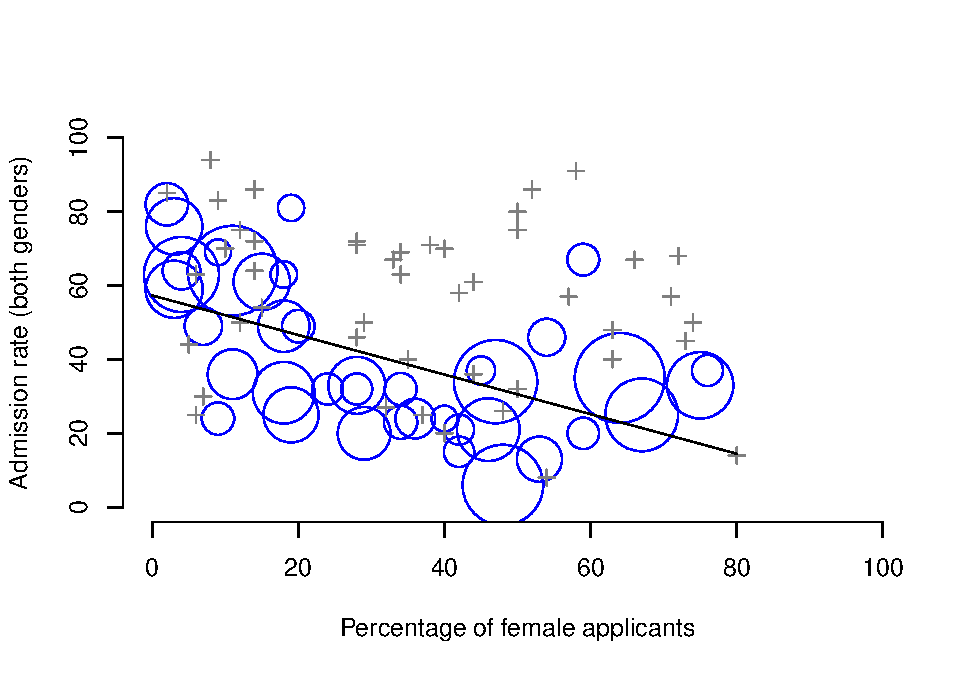
\includegraphics{schuster-statistics-remix_files/figure-latex/berkeley-1.pdf}
\caption{\label{fig:berkeley}The Berkeley 1973 college admissions data. This figure plots the admission rate for the 85 departments that had at least one female applicant, as a function of the percentage of applicants that were female. The plot is a redrawing of Figure 1 from \citet{Bickel1975}. Circles plot departments with more than 40 applicants; the area of the circle is proportional to the total number of applicants. The crosses plot department with fewer than 40 applicants.}
\end{figure}

Before leaving this topic entirely, I want to point out something else really critical that is often overlooked in a research methods class. Statistics only solves \emph{part} of the problem. Remember that we started all this with the concern that Berkeley's admissions processes might be unfairly biased against female applicants. When we looked at the ``aggregated'' data, it did seem like the university was discriminating against women, but when we ``disaggregate'' and looked at the individual behaviour of all the departments, it turned out that the actual departments were, if anything, slightly biased in favour of women. The gender bias in total admissions was caused by the fact that women tended to self-select for harder departments. From a legal perspective, that would probably put the university in the clear. Postgraduate admissions are determined at the level of the individual department (and there are good reasons to do that), and at the level of individual departments, the decisions are more or less unbiased (the weak bias in favour of females at that level is small, and not consistent across departments). Since the university can't dictate which departments people choose to apply to, and the decision making takes place at the level of the department it can hardly be held accountable for any biases that those choices produce.

That was the basis for my somewhat glib remarks earlier, but that's not exactly the whole story, is it? After all, if we're interested in this from a more sociological and psychological perspective, we might want to ask \emph{why} there are such strong gender differences in applications. Why do males tend to apply to engineering more often than females, and why is this reversed for the English department? And why is it it the case that the departments that tend to have a female-application bias tend to have lower overall admission rates than those departments that have a male-application bias? Might this not still reflect a gender bias, even though every single department is itself unbiased? It might. Suppose, hypothetically, that males preferred to apply to ``hard sciences'' and females prefer ``humanities''. And suppose further that the reason for why the humanities departments have low admission rates is because the government doesn't want to fund the humanities (Ph.D.~places, for instance, are often tied to government funded research projects). Does that constitute a gender bias? Or just an unenlightened view of the value of the humanities? What if someone at a high level in the government cut the humanities funds because they felt that the humanities are ``useless chick stuff''. That seems pretty \emph{blatantly} gender biased. None of this falls within the purview of statistics, but it matters to the research project. If you're interested in the overall structural effects of subtle gender biases, then you probably want to look at \emph{both} the aggregated and disaggregated data. If you're interested in the decision making process at Berkeley itself then you're probably only interested in the disaggregated data.

In short there are a lot of critical questions that you can't answer with statistics, but the answers to those questions will have a huge impact on how you analyse and interpret data. And this is the reason why you should always think of statistics as a \emph{tool} to help you learn about your data, no more and no less. It's a powerful tool to that end, but there's no substitute for careful thought.

\hypertarget{studydesign}{%
\section{A brief introduction to research design}\label{studydesign}}

Text by \citet{Navarro2018}

\begin{quote}
\emph{To consult the statistician after an experiment is finished is often merely to ask him to conduct a post mortem examination. He can perhaps say what the experiment died of.}

-- Sir Ronald Fisher\footnote{Presidential Address to the First Indian Statistical Congress, 1938. Source: \url{http://en.wikiquote.org/wiki/Ronald_Fisher}}
\end{quote}

Note that this section is ``special'' in two ways. Firstly, it's much more psychology-specific than the later chapters. Secondly, it focuses much more heavily on the scientific problem of research methodology, and much less on the statistical problem of data analysis. Nevertheless, the two problems are related to one another, so it's traditional for stats textbooks to discuss the problem in a little detail. This chapter relies heavily on \citet{Campbell1963} for the discussion of study design, and \citet{Stevens1946} for the discussion of scales of measurement. Later versions will attempt to be more precise in the citations.

\hypertarget{some-thoughts-about-psychological-measurement}{%
\subsection{Some thoughts about psychological measurement}\label{some-thoughts-about-psychological-measurement}}

Measurement itself is a subtle concept, but basically it comes down to finding some way of assigning numbers, or labels, or some other kind of well-defined descriptions to ``stuff''. So, any of the following would count as a psychological measurement:

\begin{itemize}
\tightlist
\item
  My \textbf{age} is \emph{33 years}.
\item
  I \emph{do not} \textbf{like anchovies}.
\item
  My \textbf{chromosomal gender} is \emph{male}.
\item
  My \textbf{self-identified gender} is \emph{male}.\footnote{Well\ldots{} now this is awkward, isn't it? This section is one of the oldest parts of the book, and it's outdated in a rather embarrassing way. I wrote this in 2010, at which point all of those facts \emph{were} true. Revisiting this in 2018\ldots{} well I'm not 33 any more, but that's not surprising I suppose. I can't imagine my chromosomes have changed, so I'm going to guess my karyotype was then and is now XY. The self-identified gender, on the other hand\ldots{} ah. I suppose the fact that the title page now refers to me as Danielle rather than Daniel might possibly be a giveaway, but I don't typically identify as ``male'' on a gender questionnaire these days, and I prefer \emph{``she/her''} pronouns as a default (it's a long story)! I did think a little about how I was going to handle this in the book, actually. The book has a somewhat distinct authorial voice to it, and I feel like it would be a rather different work if I went back and wrote everything as Danielle and updated all the pronouns in the work. Besides, it would be a lot of work, so I've left my name as ``Dan'' throughout the book, and in ant case ``Dan'' is a perfectly good nickname for ``Danielle'', don't you think? In any case, it's not a big deal. I only wanted to mention it to make life a little easier for readers who aren't sure how to refer to me. I still don't like anchovies though :-)}
\end{itemize}

In the short list above, the \textbf{bolded part} is ``the thing to be measured'', and the \emph{italicised part} is ``the measurement itself''. In fact, we can expand on this a little bit, by thinking about the set of possible measurements that could have arisen in each case:

\begin{itemize}
\tightlist
\item
  My \textbf{age} (in years) could have been \emph{0, 1, 2, 3 \ldots{}}, etc. The upper bound on what my age could possibly be is a bit fuzzy, but in practice you'd be safe in saying that the largest possible age is \emph{150}, since no human has ever lived that long.
\item
  When asked if I \textbf{like anchovies}, I might have said that \emph{I do}, or \emph{I do not}, or \emph{I have no opinion}, or \emph{I sometimes do}.
\item
  My \textbf{chromosomal gender} is almost certainly going to be \emph{male (XY)} or \emph{female (XX)}, but there are a few other possibilities. I could also have \emph{Klinfelter's syndrome (XXY)}, which is more similar to male than to female. And I imagine there are other possibilities too.
\item
  My \textbf{self-identified gender} is also very likely to be \emph{male} or \emph{female}, but it doesn't have to agree with my chromosomal gender. I may also choose to identify with \emph{neither}, or to explicitly call myself \emph{transgender}.
\end{itemize}

As you can see, for some things (like age) it seems fairly obvious what the set of possible measurements should be, whereas for other things it gets a bit tricky. But I want to point out that even in the case of someone's age, it's much more subtle than this. For instance, in the example above, I assumed that it was okay to measure age in years. But if you're a developmental psychologist, that's way too crude, and so you often measure age in \emph{years and months} (if a child is 2 years and 11 months, this is usually written as ``2;11''). If you're interested in newborns, you might want to measure age in \emph{days since birth}, maybe even \emph{hours since birth}. In other words, the way in which you specify the allowable measurement values is important.

Looking at this a bit more closely, you might also realise that the concept of ``age'' isn't actually all that precise. In general, when we say ``age'' we implicitly mean ``the length of time since birth''. But that's not always the right way to do it. Suppose you're interested in how newborn babies control their eye movements. If you're interested in kids that young, you might also start to worry that ``birth'' is not the only meaningful point in time to care about. If Baby Alice is born 3 weeks premature and Baby Bianca is born 1 week late, would it really make sense to say that they are the ``same age'' if we encountered them ``2 hours after birth''? In one sense, yes: by social convention, we use birth as our reference point for talking about age in everyday life, since it defines the amount of time the person has been operating as an independent entity in the world, but from a scientific perspective that's not the only thing we care about. When we think about the biology of human beings, it's often useful to think of ourselves as organisms that have been growing and maturing since conception, and from that perspective Alice and Bianca aren't the same age at all. So you might want to define the concept of ``age'' in two different ways: the length of time since conception, and the length of time since birth. When dealing with adults, it won't make much difference, but when dealing with newborns it might.

Moving beyond these issues, there's the question of methodology. What specific ``measurement method'' are you going to use to find out someone's age? As before, there are lots of different possibilities:

\begin{itemize}
\tightlist
\item
  You could just ask people ``how old are you?'' The method of self-report is fast, cheap and easy, but it only works with people old enough to understand the question, and some people lie about their age.
\item
  You could ask an authority (e.g., a parent) ``how old is your child?'' This method is fast, and when dealing with kids it's not all that hard since the parent is almost always around. It doesn't work as well if you want to know ``age since conception'', since a lot of parents can't say for sure when conception took place. For that, you might need a different authority (e.g., an obstetrician).
\item
  You could look up official records, like birth certificates. This is time consuming and annoying, but it has its uses (e.g., if the person is now dead).
\end{itemize}

\hypertarget{operationalisation-defining-your-measurement}{%
\subsection{Operationalisation: defining your measurement}\label{operationalisation-defining-your-measurement}}

\href{https://youtu.be/p1zqoSSIpsg}{Video: Operationalization}

All of the ideas discussed in the previous section all relate to the concept of \textbf{\emph{operationalisation}}. To be a bit more precise about the idea, operationalisation is the process by which we take a meaningful but somewhat vague concept, and turn it into a precise measurement. The process of operationalisation can involve several different things:

\begin{itemize}
\tightlist
\item
  Being precise about what you are trying to measure. For instance, does ``age'' mean ``time since birth'' or ``time since conception'' in the context of your research?
\item
  Determining what method you will use to measure it. Will you use self-report to measure age, ask a parent, or look up an official record? If you're using self-report, how will you phrase the question?
\item
  Defining the set of the allowable values that the measurement can take. Note that these values don't always have to be numerical, though they often are. When measuring age, the values are numerical, but we still need to think carefully about what numbers are allowed. Do we want age in years, years and months, days, hours? Etc. For other types of measurements (e.g., gender), the values aren't numerical. But, just as before, we need to think about what values are allowed. If we're asking people to self-report their gender, what options to we allow them to choose between? Is it enough to allow only ``male'' or ``female''? Do you need an ``other'' option? Or should we not give people any specific options, and let them answer in their own words? And if you open up the set of possible values to include all verbal response, how will you interpret their answers?
\end{itemize}

Operationalisation is a tricky business, and there's no ``one, true way'' to do it. The way in which you choose to operationalise the informal concept of ``age'' or ``gender'' into a formal measurement depends on what you need to use the measurement for. Often you'll find that the community of scientists who work in your area have some fairly well-established ideas for how to go about it. In other words, operationalisation needs to be thought through on a case by case basis. Nevertheless, while there a lot of issues that are specific to each individual research project, there are some aspects to it that are pretty general.

Before moving on, I want to take a moment to clear up our terminology, and in the process introduce one more term. Here are four different things that are closely related to each other:

\begin{itemize}
\tightlist
\item
  \textbf{\emph{A theoretical construct}}. This is the thing that you're trying to take a measurement of, like ``age'', ``gender'' or an ``opinion''. A theoretical construct can't be directly observed, and often they're actually a bit vague.
\item
  \textbf{\emph{A measure}}. The measure refers to the method or the tool that you use to make your observations. A question in a survey, a behavioural observation or a brain scan could all count as a measure.
\item
  \textbf{\emph{An operationalisation}}. The term ``operationalisation'' refers to the logical connection between the measure and the theoretical construct, or to the process by which we try to derive a measure from a theoretical construct.
\item
  \textbf{\emph{A variable}}. Finally, a new term. A variable is what we end up with when we apply our measure to something in the world. That is, variables are the actual ``data'' that we end up with in our data sets.
\end{itemize}

In practice, even scientists tend to blur the distinction between these things, but it's very helpful to try to understand the differences.

\hypertarget{ivdv}{%
\subsection{The ``role'' of variables: predictors and outcomes}\label{ivdv}}

Okay, I've got one last piece of terminology that I need to explain to you before moving away from variables. Normally, when we do some research we end up with lots of different variables. Then, when we analyse our data we usually try to explain some of the variables in terms of some of the other variables. It's important to keep the two roles ``thing doing the explaining'' and ``thing being explained'' distinct. So let's be clear about this now. Firstly, we might as well get used to the idea of using mathematical symbols to describe variables, since it's going to happen over and over again. Let's denote the ``to be explained'' variable \(Y\), and denote the variables ``doing the explaining'' as \(X_1\), \(X_2\), etc.

Now, when we doing an analysis, we have different names for \(X\) and \(Y\), since they play different roles in the analysis. The classical names for these roles are \textbf{\emph{independent variable}} (IV) and \textbf{\emph{dependent variable}} (DV). The IV is the variable that you use to do the explaining (i.e., \(X\)) and the DV is the variable being explained (i.e., \(Y\)). The logic behind these names goes like this: if there really is a relationship between \(X\) and \(Y\) then we can say that \(Y\) depends on \(X\), and if we have designed our study ``properly'' then \(X\) isn't dependent on anything else. However, I personally find those names horrible: they're hard to remember and they're highly misleading, because (a) the IV is never actually ``independent of everything else'' and (b) if there's no relationship, then the DV doesn't actually depend on the IV. And in fact, because I'm not the only person who thinks that IV and DV are just awful names, there are a number of alternatives that I find more appealing. The terms that I'll use in these notes are \textbf{\emph{predictors}} and \textbf{\emph{outcomes}}. The idea here is that what you're trying to do is use \(X\) (the predictors) to make guesses about \(Y\) (the outcomes).\footnote{Annoyingly, though, there's a lot of different names used out there. I won't list all of them -- there would be no point in doing that -- other than to note that R often uses ``response variable'' where I've used ``outcome'', and a traditionalist would use ``dependent variable''. Sigh. This sort of terminological confusion is very common, I'm afraid.} This is summarised in Table \ref{tab:ivdv}.

\begin{table}

\caption{\label{tab:ivdv}The terminology used to distinguish between different roles that a variable can play when analysing a data set. Note that this book will tend to avoid the classical terminology in favour of the newer names.}
\centering
\begin{tabular}[t]{lll}
\toprule
role of the variable & classical name & modern name\\
\midrule
to be explained & dependent variable (DV) & outcome\\
to do the explaining & independent variable (IV) & predictor\\
\bottomrule
\end{tabular}
\end{table}

\hypertarget{researchdesigns}{%
\subsection{Experimental and non-experimental research}\label{researchdesigns}}

\href{https://youtu.be/H9uDTWD8R4M}{Video: Experimental, Quasi-, and Non-Experimental Research Designs}

One of the big distinctions that you should be aware of is the distinction between ``experimental research'' and ``non-experimental research''. When we make this distinction, what we're really talking about is the degree of control that the researcher exercises over the people and events in the study.

\hypertarget{experimental-research}{%
\subsubsection{Experimental research}\label{experimental-research}}

The key features of \textbf{\emph{experimental research}} is that the researcher controls all aspects of the study, especially what participants experience during the study. In particular, the researcher manipulates or varies the predictor variables (IVs), and then allows the outcome variable (DV) to vary naturally. The idea here is to deliberately vary the predictors (IVs) to see if they have any causal effects on the outcomes. Moreover, in order to ensure that there's no chance that something other than the predictor variables is causing the outcomes, everything else is kept constant or is in some other way ``balanced'' to ensure that they have no effect on the results. In practice, it's almost impossible to \emph{think} of everything else that might have an influence on the outcome of an experiment, much less keep it constant. The standard solution to this is \textbf{\emph{randomisation}}: that is, we randomly assign people to different groups, and then give each group a different treatment (i.e., assign them different values of the predictor variables). We'll talk more about randomisation later in this course, but for now, it's enough to say that what randomisation does is minimise (but not eliminate) the chances that there are any systematic difference between groups.

Let's consider a very simple, completely unrealistic and grossly unethical example. Suppose you wanted to find out if smoking causes lung cancer. One way to do this would be to find people who smoke and people who don't smoke, and look to see if smokers have a higher rate of lung cancer. This is \emph{not} a proper experiment, since the researcher doesn't have a lot of control over who is and isn't a smoker. And this really matters: for instance, it might be that people who choose to smoke cigarettes also tend to have poor diets, or maybe they tend to work in asbestos mines, or whatever. The point here is that the groups (smokers and non-smokers) actually differ on lots of things, not \emph{just} smoking. So it might be that the higher incidence of lung cancer among smokers is caused by something else, not by smoking per se. In technical terms, these other things (e.g.~diet) are called ``confounds'', and we'll talk about those in just a moment.

In the meantime, let's now consider what a proper experiment might look like. Recall that our concern was that smokers and non-smokers might differ in lots of ways. The solution, as long as you have no ethics, is to \emph{control} who smokes and who doesn't. Specifically, if we randomly divide participants into two groups, and force half of them to become smokers, then it's very unlikely that the groups will differ in any respect other than the fact that half of them smoke. That way, if our smoking group gets cancer at a higher rate than the non-smoking group, then we can feel pretty confident that (a) smoking does cause cancer and (b) we're murderers.

\hypertarget{causality-research-and-statistics}{%
\section{Causality, Research, and Statistics}\label{causality-research-and-statistics}}

Text by David Schuster

\href{https://youtu.be/s9itzrOlnq4}{Video: Causality}

\hypertarget{experimental-quasi-experimental-and-non-experimental-studies}{%
\subsection{Experimental, Quasi-Experimental, and Non-Experimental Studies}\label{experimental-quasi-experimental-and-non-experimental-studies}}

In this section, I would like to add a bit more precision to the general concepts explained by \citet{Navarro2018}.

Research psychology is a process of identifying constructs and describing how they relate to other constructs. We can classify research designs as experiments, quasi-experiments, and non-experiments.

Experiments are the only kind of research that shows causal relationships (that is, that construct A causes a change in construct B). So an experiment could show if smoking causes lung cancer. To do this, experiments need two things (or they are not experiments)

All experiments have a manipulation. This means that the experimenter changes something within the environment of the experiment (called an independent variable) to see if it causes a change in the outcome (called a dependent variable). For our smoking example, a manipulation would be assigning one group of participants to a lifetime of smoking and another group of participants to a lifetime of no smoking.

Experiments require random assignment. The experimenter decides when to vary the levels of the manipulation (change the manipulation) based on random assignment. Random assignment means that every participant has the same chance as being in one condition as another. For our smoking example, random assignment means each participant has a 50\% chance of being in the smoking group.

As may be clear from the smoking example, we cannot always do experiments because of ethical (it would be wrong to assign people to smoke) or practical reasons (you cannot randomly assign people to genders, for example). The solution is a quasi- or non-experimental study.

In summary: experiments are powerful because they uniquely demonstrate causality (causal relationships). However, experiments require a manipulation and random assignment, which are not always possible.

In a quasi-experimental study, there is a manipulation but no random assignment. Whenever participants are assigned to levels of a manipulation non-randomly, the research is quasi-experimental. In a quasi-experimental smoking study, we could ask people if they had smoked before and assign them to smoking or non-smoking groups based on that answer.

In summary: quasi-experiments do not require random assignment, but they do not show casual relationships.

In a non-experimental study, no manipulation is done. If you want to look at the effects of gender on lung cancer, you would simply observe (collect data on) the genders of patients. By only observing, you would not be manipulating gender.

The differences between quasi- and non-experimental studies are sometimes slight (Pedhauzer \& Schmelkin, 1991); if the researcher is manipulating an IV, then the work is quasi-experimental.

In summary: non-experimental studies are observational. Like quasi-experimental studies, they do not show causal relationships.

It's worth repeating that only experiments demonstrate causality. Quasi- and non-experiments can show that a relationship exists but do not say whether one variable causes the other. Any non-causal relationship has three possible explanations:

\begin{enumerate}
\def\labelenumi{\arabic{enumi}.}
\tightlist
\item
  A \(\rightarrow\) B one variable causes another; in an experiment, this is the only explanation
\item
  B \(\leftarrow\) A the relationship is reversed; the first variable is actually the outcome
\item
  C \(\rightarrow\) A; C \(\rightarrow\) B a third variable exists that was not measured in the study; the third variable causes a change in both A and B. There are many `C' variables, potentially.
\end{enumerate}

In a non-experimental smoking study, you could not say whether smoking causes lung cancer or people who are predisposed to lung cancer are more likely to smoke. A third possibility is that a separate, third variable causes both lung cancer and a desire to smoke.

\hypertarget{demonstrating-causality}{%
\subsection{Demonstrating Causality}\label{demonstrating-causality}}

In the 19th century, John Stewart Mill said that we could be satisfied that a relationship is causal if the following three things could be demonstrated:

\begin{enumerate}
\def\labelenumi{\arabic{enumi}.}
\tightlist
\item
  The cause preceded the effect
\item
  The cause was related to the effect
\item
  We can find no plausible alternative explanation for the effect other than the cause
\end{enumerate}

Experiments aim to identify causal relationships by manipulating something, observing the outcome, seeing a relationship, and using various methods to reduce other explanations.

\hypertarget{statistics-and-causality}{%
\subsection{Statistics and Causality}\label{statistics-and-causality}}

Statistics are an important tool for establishing causality, but it's important to know that the choice of statistical technique does not affect the level of causal evidence; demonstrating causality is the job of the research design, not the statistics.

A common misconception arises from the term correlational research design, which people use as a label for quasi-experimental and non-experimental research. It is easy to confuse this term with correlation which is a statistical technique.

Recall that statistics has two branches: Descriptive stats provides tools to summarize variability. Inferential stats provides tools for generalizing samples to populations.

To demonstrate causality, we need to satisfy Mill's second requirement. Inferential statistics can help us do that. Two techniques are particularly useful: correlation (and its statistic r) and the t¬-test (and its statistic, t). Next, we will see how these techniques work.

\hypertarget{validity-and-reliability}{%
\subsection{Validity and Reliability}\label{validity-and-reliability}}

Text by David Schuster

\hypertarget{define-validity-and-reliability}{%
\subsubsection{Define validity and reliability}\label{define-validity-and-reliability}}

Reliability and validity are fundamental to critiquing psychological research and to developing your own high-quality research. There are different types of validity and reliability that are relevant to us, which sometimes confuses people. Because of this, introductory textbooks often present convoluted definitions of these concepts. Fortunately, the real definitions are simple:

Reliability means consistency. Something is reliable if it is consistent. The more consistency, the more reliability.

Validity means truth. Something is valid if it is true. Truth is either-or; there is no such thing as ``more true'' or ``less true.''

In other words, good psychological science requires certain types of consistency and for some of the claims we make to be true. Next, we will look at the specific kinds of reliability and validity that are important for scientists.

\hypertarget{types-of-consistency-types-of-reliability}{%
\subsubsection{Types of consistency = Types of Reliability}\label{types-of-consistency-types-of-reliability}}

\href{https://youtu.be/EatmTWbD4uo}{Reliability}

Here are arguably the three most important types of reliability:

\begin{longtable}[]{@{}
  >{\raggedright\arraybackslash}p{(\columnwidth - 6\tabcolsep) * \real{0.06}}
  >{\raggedright\arraybackslash}p{(\columnwidth - 6\tabcolsep) * \real{0.55}}
  >{\raggedright\arraybackslash}p{(\columnwidth - 6\tabcolsep) * \real{0.23}}
  >{\raggedright\arraybackslash}p{(\columnwidth - 6\tabcolsep) * \real{0.16}}@{}}
\toprule
Type of Reliability & Situation & Definition & How to assess \\
\midrule
\endhead
Test-retest & You administer a measure to a participant, then wait some period of time, and give them the test again. The participant's true score on the measure has not changed (e.g., IQ, personality). & The extent to which a measure is consistent across different administrations & Look for a correlation between the two administrations \\
Interrater & A measure involves two or more raters who record subjective observations (e.g., counting the number of times a participant has a tic, counting the number of times a married couple shows affection) & The extent to which two observers are consistent in their ratings & Look for a correlation between the two raters \\
Internal consistency & You are measuring a construct using several items (e.g., five items all rating your enjoyment of a course) & The extent to which items on a measure are consistent with each other; expected if the items measure the same construct & Cronbach's alpha (.7 is acceptable, .8 is good, and .9 is excellent) \\
\bottomrule
\end{longtable}

\hypertarget{validity-is-a-property-of-inferences}{%
\subsubsection{Validity is a property of inferences}\label{validity-is-a-property-of-inferences}}

\href{https://youtu.be/mxZxGttf6sE}{Video: Validity \& Threats}

Validity is a specific kind of truth. Validity is the truth of an inference, or a claim. In other words, validity is a property of inferences. An inference (a claim) is valid if it is true.

For example, I could claim that the earth is round. Hopefully, it is a claim that you accept as being true. If you agree, then you could label my claim as valid.

Validity in research is frequently misunderstood, which leads to bizarre and confusing definitions of validity. There is no such thing as ``a valid study.'' Only claims about the study are valid or not. There is also no such thing as ``a valid researcher.'' A researcher can make claims. Only the researcher's claims are valid or not. There is also no such thing as ``more valid'' or ``increasing validity.'' Validity is truth of a claim. Either a claim is true, or it is not.

For better or for worse, we usually don't know with 100\% certainty if a claim is true or false (if we did, we wouldn't need the research). Therefore, research methods get very interesting when we listen to other researcher's claims and then debate if we agree with them or not. When we do this, we are evaluating the validity of claims made about the study. Next, let's look at different types of claims (inferences) that are made in research.

\hypertarget{types-of-inferences-in-a-study-types-of-validity}{%
\subsubsection{Types of inferences in a study = Types of validity}\label{types-of-inferences-in-a-study-types-of-validity}}

Here are some of the most important types of validity.

\begin{longtable}[]{@{}
  >{\raggedright\arraybackslash}p{(\columnwidth - 6\tabcolsep) * \real{0.30}}
  >{\raggedright\arraybackslash}p{(\columnwidth - 6\tabcolsep) * \real{0.25}}
  >{\raggedright\arraybackslash}p{(\columnwidth - 6\tabcolsep) * \real{0.19}}
  >{\raggedright\arraybackslash}p{(\columnwidth - 6\tabcolsep) * \real{0.27}}@{}}
\toprule
Type of Validity & Type of Claim & Definition & Example claim \\
\midrule
\endhead
Construct validity & The study operations represent the constructs of interest & The truth of claims that study operations match study constructs & ``The Stanford-Binet was used to measure IQ'' \\
Internal validity & The study IV caused a change in the study DV & The truth of claims that the IV causes changes in the DV & ``The control group reported lower levels of stress than the experimental group, suggesting that the manipulation raised stress.'' \\
External validity & The study results apply to situation X & The truth of claims that the findings will apply as participants/units/variables/settings change. & ``Although data were collected from college students, a similar effect would be expected in working adults.'' \\
Statistical conclusion validity & The statistical analysis was significant or not significant & The truth of claims about the size and direction of the relationship between the IV and the DV. Or, that the statistical results are correct. & ``p \textless{} .05, indicating a significant difference'' \\
\bottomrule
\end{longtable}

Finally, you might encounter these other types of validity, but they are less clearly defined and evaluated:

\begin{itemize}
\tightlist
\item
  Content validity: The truth of claims that a measure adequately samples (includes the important elements of) the domain of interest. For example, if IQ includes both verbal and math ability, an IQ test would need to have both verbal and math items.
\item
  Face validity: The truth of claims that a study operation ``seems like'' the construct. For example, a study about distractions from mobile devices might not support claims of ``seeming real'' if the phone in the study is a paper mockup.
\item
  Criterion validity: The truth of claims that a measure can predict or correlate with some outcome of interest. A personality test as part of a job application would have criterion validity if it predicted applicants' success in the job.
\end{itemize}

\hypertarget{threats-to-validity}{%
\subsubsection{Threats to validity}\label{threats-to-validity}}

Threats to validity are specific reasons why an inference about a study is wrong. They can help us anticipate problems in the design of our own research. The best way to address threats to validity is to change the design of our research. Understanding threats to validity also helps you critique research done by others.

\hypertarget{introR}{%
\chapter{Getting started with R}\label{introR}}

\begin{quote}
\emph{Robots are nice to work with.}

--Roger Zelazny\footnote{Source: \emph{Dismal Light} (1968).}
\end{quote}

In this chapter I'll discuss how to get started in R. I'll briefly talk about how to download and install R, but most of the chapter will be focused on getting you started typing R commands. Our goal in this chapter is not to learn any statistical concepts: we're just trying to learn the basics of how R works and get comfortable interacting with the system. To do this, we'll spend a bit of time using R as a simple calculator, since that's the easiest thing to do with R. In doing so, you'll get a bit of a feel for what it's like to work in R. From there I'll introduce some very basic programming ideas: in particular, I'll talk about the idea of defining \emph{variables} to store information, and a few things that you can do with these variables.

However, before going into any of the specifics, it's worth talking a little about why you might want to use R at all. Given that you're reading this, you've probably got your own reasons. However, if those reasons are ``because that's what my stats class uses'', it might be worth explaining a little why your lecturer has chosen to use R for the class. Of course, I don't really know why \emph{other} people choose R, so I'm really talking about why I use it.

\begin{itemize}
\tightlist
\item
  It's sort of obvious, but worth saying anyway: doing your statistics on a computer is faster, easier and more powerful than doing statistics by hand. Computers excel at mindless repetitive tasks, and a lot of statistical calculations are both mindless and repetitive. For most people, the only reason to ever do statistical calculations with pencil and paper is for learning purposes. In my class I do occasionally suggest doing some calculations that way, but the only real value to it is pedagogical. It does help you to get a ``feel'' for statistics to do some calculations yourself, so it's worth doing it once. But only once!
\item
  Doing statistics in a spreadsheet (e.g., Microsoft Excel) is generally a bad idea in the long run. Although many people are likely feel more familiar with them, spreadsheets are very limited in terms of what analyses they allow you do. If you get into the habit of trying to do your real life data analysis using spreadsheets, then you've dug yourself into a very deep hole.
\item
  Avoiding proprietary software is a very good idea. There are a lot of commercial packages out there that you can buy, some of which I like and some of which I don't. They're usually very glossy in their appearance, and generally very powerful (much more powerful than spreadsheets). However, they're also very expensive: usually, the company sells ``student versions'' (crippled versions of the real thing) very cheaply; they sell full powered ``educational versions'' at a price that makes me wince; and they sell commercial licences with a staggeringly high price tag. The business model here is to suck you in during your student days, and then leave you dependent on their tools when you go out into the real world. It's hard to blame them for trying, but personally I'm not in favour of shelling out thousands of dollars if I can avoid it. And you can avoid it: if you make use of packages like R that are open source and free, you never get trapped having to pay exorbitant licensing fees.
\item
  Something that you might not appreciate now, but will love later on if you do anything involving data analysis, is the fact that R is highly extensible. When you download and install R, you get all the basic ``packages'', and those are very powerful on their own. However, because R is so open and so widely used, it's become something of a standard tool in statistics, and so lots of people write their own packages that extend the system. And these are freely available too. One of the consequences of this, I've noticed, is that if you open up an advanced textbook (a recent one, that is) rather than introductory textbooks, is that a \emph{lot} of them use R. In other words, if you learn how to do your basic statistics in R, then you're a lot closer to being able to use the state of the art methods than you would be if you'd started out with a ``simpler'' system: so if you want to become a genuine expert in psychological data analysis, learning R is a very good use of your time.
\item
  Related to the previous point: R is a real programming language. As you get better at using R for data analysis, you're also learning to program. To some people this might seem like a bad thing, but in truth, programming is a core research skill across a lot of the social and behavioural sciences. Think about how many surveys and experiments are done online, or presented on computers. Think about all those online social environments which you might be interested in studying; and maybe collecting data from in an automated fashion. Think about artificial intelligence systems, computer vision and speech recognition. If any of these are things that you think you might want to be involved in -- as someone ``doing research in psychology'', that is -- you'll need to know a bit of programming. And if you don't already know how to program, then learning how to do statistics using R is a nice way to start.
\end{itemize}

Those are the main reasons I use R. It's not without its flaws: it's not easy to learn, and it has a few very annoying quirks to it that we're all pretty much stuck with, but on the whole I think the strengths outweigh the weakness; more so than any other option I've encountered so far.

\hypertarget{gettingR}{%
\section{Installing R}\label{gettingR}}

Okay, enough with the sales pitch. Let's get started. Just as with any piece of software, R needs to be installed on a ``computer'', which is a magical box that does cool things and delivers free ponies. Or something along those lines: I may be confusing computers with the iPad marketing campaigns. Anyway, R is freely distributed online, and you can download it from the R homepage, which is:

\begin{quote}
\url{http://cran.r-project.org/}
\end{quote}

At the top of the page -- under the heading ``Download and Install R'' -- you'll see separate links for Windows users, Mac users, and Linux users. If you follow the relevant link, you'll see that the online instructions are pretty self-explanatory, but I'll walk you through the installation anyway. As of this writing, the current version of R is 3.0.2 (``Frisbee Sailing"), but they usually issue updates every six months, so you'll probably have a newer version.\footnote{Although R is updated frequently, it doesn't usually make much of a difference for the sort of work we'll do in this book. In fact, during the writing of the book I upgraded several times, and didn't have to change much except these sections describing the downloading.}

\hypertarget{installing-r-on-a-windows-computer}{%
\subsection{Installing R on a Windows computer}\label{installing-r-on-a-windows-computer}}

The CRAN homepage changes from time to time, and it's not particularly pretty, or all that well-designed quite frankly. But it's not difficult to find what you're after. In general you'll find a link at the top of the page with the text ``Download R for Windows''. If you click on that, it will take you to a page that offers you a few options. Again, at the very top of the page you'll be told to click on a link that says to click here if you're installing R for the first time. That's probably what you want. This will take you to a page that has a prominent link at the top called ``Download R 3.0.2 for Windows''. That's the one you want. Click on that and your browser should start downloading a file called \texttt{R-3.0.2-win.exe}, or whatever the equivalent version number is by the time you read this. The file for version 3.0.2 is about 54MB in size, so it may take some time depending on how fast your internet connection is. Once you've downloaded the file, double click to install it. As with any software you download online, Windows will ask you some questions about whether you trust the file and so on. After you click through those, it'll ask you where you want to install it, and what components you want to install. The default values should be fine for most people, so again, just click through. Once all that is done, you should have R installed on your system. You can access it from the Start menu, or from the desktop if you asked it to add a shortcut there. You can now open up R in the usual way if you want to, but what I'm going to suggest is that instead of doing that you should now install RStudio (see Section \ref{installingrstudio} for instructions).

\hypertarget{installing-r-on-a-mac}{%
\subsection{Installing R on a Mac}\label{installing-r-on-a-mac}}

When you click on the Mac OS X link, you should find yourself on a page with the title ``R for Mac OS X''. The vast majority of Mac users will have a fairly recent version of the operating system: as long as you're running Mac OS X 10.6 (Snow Leopard) or higher, then you'll be fine.\footnote{If you're running an older version of the Mac OS, then you need to follow the link to the ``old'' page (\url{http://cran.r-project.org/bin/macosx/old/}). You should be able to find the installer file that you need at the bottom of the page.} There's a fairly prominent link on the page called ``R-3.0.2.pkg'', which is the one you want. Click on that link and you'll start downloading the installer file, which is (not surprisingly) called \texttt{R-3.0.2.pkg}. It's about 61MB in size, so the download can take a while on slower internet connections.

Once you've downloaded \texttt{R-3.0.2.pkg}, all you need to do is open it by double clicking on the package file. The installation should go smoothly from there: just follow all the instructions just like you usually do when you install something. Once it's finished, you'll find a file called \texttt{R.app} in the Applications folder. You can now open up R in the usual way\footnote{Tip for advanced Mac users. You can run R from the terminal if you want to. The command is just ``R''. It behaves like the normal desktop version, except that help documentation behaves like a ``man'' page instead of opening in a new window.} if you want to, but what I'm going to suggest is that instead of doing that you should now install RStudio (see Section \ref{installingrstudio} for instructions).

\hypertarget{installing-r-on-a-linux-computer}{%
\subsection{Installing R on a Linux computer}\label{installing-r-on-a-linux-computer}}

If you're successfully managing to run a Linux box, regardless of what distribution, then you should find the instructions on the website easy enough. You can compile R from source yourself if you want, or install it through your package management system, which will probably have R in it.
Alternatively, the CRAN site has precompiled binaries for Debian, Red Hat, Suse and Ubuntu and has separate instructions for each. Once you've got R installed, you can run it from the command line just by typing \texttt{R}. However, if you're feeling envious of Windows and Mac users for their fancy GUIs, you can download RStudio too (see Section \ref{installingrstudio} for instructions).

\hypertarget{installingrstudio}{%
\subsection{Downloading and installing RStudio}\label{installingrstudio}}

Okay, so regardless of what operating system you're using, the last thing that I told you to do is to download RStudio. To understand why I've suggested this, you need to understand a little bit more about R itself. The term R doesn't really refer to a specific application on your computer. Rather, it refers to the underlying statistical language. You can use this language through lots of different applications. When you install R initially, it comes with one application that lets you do this: it's the R.exe application on a Windows machine, and the R.app application on a Mac. But that's not the only way to do it. There are lots of different applications that you can use that will let you interact with R. One of those is called RStudio, and it's the one I'm going to suggest that you use. RStudio provides a clean, professional interface to R that I find much nicer to work with than either the Windows or Mac defaults. Like R itself, RStudio is free software: you can find all the details on their webpage. In the meantime, you can download it here:

\begin{quote}
\url{http://www.RStudio.org/}
\end{quote}

When you visit the RStudio website, you'll probably be struck by how much cleaner and simpler it is than the CRAN website,\footnote{This is probably no coincidence: the people who design and distribute the core R language itself are focused on technical stuff. And sometimes they almost seem to forget that there's an actual human user at the end. The people who design and distribute RStudio are focused on user interface. They want to make R as usable as possible. The two websites reflect that difference.} and how obvious it is what you need to do: click the big green button that says ``Download''.

When you click on the download button on the homepage it will ask you to choose whether you want the desktop version or the server version. You want the desktop version. After choosing the desktop version it will take you to a page \url{http://www.RStudio.org/download/desktop}) that shows several possible downloads: there's a different one for each operating system. However, the nice people at RStudio have designed the webpage so that it automatically recommends the download that is most appropriate for your computer. Click on the appropriate link, and the RStudio installer file will start downloading.

Once it's finished downloading, open the installer file in the usual way to install RStudio. After it's finished installing, you can start R by opening RStudio. You don't need to open R.app or R.exe in order to access R. RStudio will take care of that for you. To illustrate what RStudio looks like, Figure \ref{fig:RStudio} shows a screenshot of an R session in progress. In this screenshot, you can see that it's running on a Mac, but it looks almost identical no matter what operating system you have. The Windows version looks more like a Windows application (e.g., the menus are attached to the application window and the colour scheme is slightly different), but it's more or less identical. There are a few minor differences in where things are located in the menus (I'll point them out as we go along) and in the shortcut keys, because RStudio is trying to ``feel'' like a proper Mac application or a proper Windows application, and this means that it has to change its behaviour a little bit depending on what computer it's running on. Even so, these differences are very small: I started out using the Mac version of RStudio and then started using the Windows version as well in order to write these notes.

\begin{figure}
\centering
\includegraphics{/Users/dave/Documents/GitHub/stats-remix-advanced/bookdown/img/introR/RStudio2.png}
\caption{\label{fig:RStudio}An R session in progress running through RStudio. The picture shows RStudio running on a Mac, but the Windows interface is almost identical.}
\end{figure}

The only ``shortcoming'' I've found with RStudio is that -- as of this writing -- it's still a work in progress. The ``problem'' is that they keep improving it. New features keep turning up the more recent releases, so there's a good chance that by the time you read this book there will be a version out that has some really neat things that weren't in the version that I'm using now.

\hypertarget{startingR}{%
\subsection{Starting up R}\label{startingR}}

One way or another, regardless of what operating system you're using and regardless of whether you're using RStudio, or the default GUI, or even the command line, it's time to open R and get started. When you do that, the first thing you'll see (assuming that you're looking at the \textbf{\emph{R console}}, that is) is a whole lot of text that doesn't make much sense. It should look something like this:

\begin{verbatim}
R version 3.0.2 (2013-09-25) -- "Frisbee Sailing"
Copyright (C) 2013 The R Foundation for Statistical Computing
Platform: x86_64-apple-darwin10.8.0 (64-bit)

R is free software and comes with ABSOLUTELY NO WARRANTY.
You are welcome to redistribute it under certain conditions.
Type 'license()' or 'licence()' for distribution details.

  Natural language support but running in an English locale

R is a collaborative project with many contributors.
Type 'contributors()' for more information and
'citation()' on how to cite R or R packages in publications.

Type 'demo()' for some demos, 'help()' for on-line help, or
'help.start()' for an HTML browser interface to help.
Type 'q()' to quit R.

> 
\end{verbatim}

Most of this text is pretty uninteresting, and when doing real data analysis you'll never really pay much attention to it. The important part of it is this\ldots{}

\begin{verbatim}
>
\end{verbatim}

\ldots{} which has a flashing cursor next to it. That's the \textbf{\emph{command prompt}}. When you see this, it means that R is waiting patiently for you to do something!

\hypertarget{firstcommand}{%
\section{Typing commands at the R console}\label{firstcommand}}

One of the easiest things you can do with R is use it as a simple calculator, so it's a good place to start. For instance, try typing \texttt{10\ +\ 20}, and hitting enter.\footnote{Seriously. If you're in a position to do so, open up R and start typing. The simple act of typing it rather than ``just reading'' makes a big difference. It makes the concepts more concrete, and it ties the abstract ideas (programming and statistics) to the actual context in which you need to use them. Statistics is something you \emph{do}, not just something you read about in a textbook.} When you do this, you've entered a \textbf{\emph{command}}, and R will ``execute'' that command. What you see on screen now will be this:

\begin{Shaded}
\begin{Highlighting}[]
\SpecialCharTok{\textgreater{}} \DecValTok{10} \SpecialCharTok{+} \DecValTok{20}
\NormalTok{[}\DecValTok{1}\NormalTok{] }\DecValTok{30}
\end{Highlighting}
\end{Shaded}

Not a lot of surprises in this extract. But there's a few things worth talking about, even with such a simple example. Firstly, it's important that you understand how to read the extract. In this example, what \emph{I} typed was the \texttt{10\ +\ 20} part. I didn't type the \texttt{\textgreater{}} symbol: that's just the R command prompt and isn't part of the actual command. And neither did I type the \texttt{{[}1{]}\ 30} part. That's what R printed out in response to my command.

Secondly, it's important to understand how the output is formatted. Obviously, the correct answer to the sum \texttt{10\ +\ 20} is \texttt{30}, and not surprisingly R has printed that out as part of its response. But it's also printed out this \texttt{{[}1{]}} part, which probably doesn't make a lot of sense to you right now. You're going to see that a lot. I'll talk about what this means in a bit more detail later on, but for now you can think of \texttt{{[}1{]}\ 30} as if R were saying ``the answer to the 1st question you asked is 30''. That's not quite the truth, but it's close enough for now. And in any case it's not really very interesting at the moment: we only asked R to calculate one thing, so obviously there's only one answer printed on the screen. Later on this will change, and the \texttt{{[}1{]}} part will start to make a bit more sense. For now, I just don't want you to get confused or concerned by it.

\hypertarget{an-important-digression-about-formatting}{%
\subsection{An important digression about formatting}\label{an-important-digression-about-formatting}}

Now that I've taught you these rules I'm going to change them pretty much immediately. That is because I want you to be able to copy code from the book directly into R if if you want to test things or conduct your own analyses. However, if you copy this kind of code (that shows the command prompt and the results) directly into R you will get an error

\begin{Shaded}
\begin{Highlighting}[]
\SpecialCharTok{\textgreater{}} \DecValTok{10} \SpecialCharTok{+} \DecValTok{20}
\NormalTok{[}\DecValTok{1}\NormalTok{] }\DecValTok{30}
\end{Highlighting}
\end{Shaded}

\begin{verbatim}
## Error: <text>:1:1: unexpected '>'
## 1: >
##     ^
\end{verbatim}

So instead, I'm going to provide code in a slightly different format so that it looks like this\ldots{}

\begin{Shaded}
\begin{Highlighting}[]
\DecValTok{10} \SpecialCharTok{+} \DecValTok{20}
\end{Highlighting}
\end{Shaded}

\begin{verbatim}
## [1] 30
\end{verbatim}

There are two main differences.

\begin{itemize}
\tightlist
\item
  In your console, you type after the \textgreater, but from now I I won't show the command prompt in the book.\\
\item
  In the book, output is commented out with \#\#, in your console it appears directly after your code.
\end{itemize}

These two differences mean that if you're working with an electronic version of the book, you can easily copy code out of the book and into the console.

So for example if you copied the two lines of code from the book you'd get this

\begin{Shaded}
\begin{Highlighting}[]
\DecValTok{10} \SpecialCharTok{+} \DecValTok{20}
\end{Highlighting}
\end{Shaded}

\begin{verbatim}
## [1] 30
\end{verbatim}

\begin{Shaded}
\begin{Highlighting}[]
\DocumentationTok{\#\# [1] 30}
\end{Highlighting}
\end{Shaded}

\hypertarget{be-very-careful-to-avoid-typos}{%
\subsection{Be very careful to avoid typos}\label{be-very-careful-to-avoid-typos}}

Before we go on to talk about other types of calculations that we can do with R, there's a few other things I want to point out. The first thing is that, while R is good software, it's still software. It's pretty stupid, and because it's stupid it can't handle typos. It takes it on faith that you meant to type \emph{exactly} what you did type. For example, suppose that you forgot to hit the shift key when trying to type \texttt{+}, and as a result your command ended up being \texttt{10\ =\ 20} rather than \texttt{10\ +\ 20}. Here's what happens:

\begin{Shaded}
\begin{Highlighting}[]
\DecValTok{10} \OtherTok{=} \DecValTok{20}
\end{Highlighting}
\end{Shaded}

\begin{verbatim}
## Error in 10 = 20: invalid (do_set) left-hand side to assignment
\end{verbatim}

What's happened here is that R has attempted to interpret \texttt{10\ =\ 20} as a command, and spits out an error message because the command doesn't make any sense to it. When a \emph{human} looks at this, and then looks down at his or her keyboard and sees that \texttt{+} and \texttt{=} are on the same key, it's pretty obvious that the command was a typo. But R doesn't know this, so it gets upset. And, if you look at it from its perspective, this makes sense. All that R ``knows'' is that \texttt{10} is a legitimate number, \texttt{20} is a legitimate number, and \texttt{=} is a legitimate part of the language too. In other words, from its perspective this really does look like the user meant to type \texttt{10\ =\ 20}, since all the individual parts of that statement are legitimate and it's too stupid to realise that this is probably a typo. Therefore, R takes it on faith that this is exactly what you meant\ldots{} it only ``discovers'' that the command is nonsense when it tries to follow your instructions, typo and all. And then it whinges, and spits out an error.

Even more subtle is the fact that some typos won't produce errors at all, because they happen to correspond to ``well-formed'' R commands. For instance, suppose that not only did I forget to hit the shift key when trying to type \texttt{10\ +\ 20}, I also managed to press the key next to one I meant do. The resulting typo would produce the command \texttt{10\ -\ 20}. Clearly, R has no way of knowing that you meant to \emph{add} 20 to 10, not \emph{subtract} 20 from 10, so what happens this time is this:

\begin{Shaded}
\begin{Highlighting}[]
\DecValTok{10} \SpecialCharTok{{-}} \DecValTok{20}
\end{Highlighting}
\end{Shaded}

\begin{verbatim}
## [1] -10
\end{verbatim}

In this case, R produces the right answer, but to the the wrong question.

To some extent, I'm stating the obvious here, but it's important. The people who wrote R are smart. You, the user, are smart. But R itself is dumb. And because it's dumb, it has to be mindlessly obedient. It does \emph{exactly} what you ask it to do. There is no equivalent to ``autocorrect'' in R, and for good reason. When doing advanced stuff -- and even the simplest of statistics is pretty advanced in a lot of ways -- it's dangerous to let a mindless automaton like R try to overrule the human user. But because of this, it's your responsibility to be careful. Always make sure you type \emph{exactly what you mean}. When dealing with computers, it's not enough to type ``approximately'' the right thing. In general, you absolutely \emph{must} be precise in what you say to R \ldots{} like all machines it is too stupid to be anything other than absurdly literal in its interpretation.

\hypertarget{r-is-a-bit-flexible-with-spacing}{%
\subsection{R is (a bit) flexible with spacing}\label{r-is-a-bit-flexible-with-spacing}}

Of course, now that I've been so uptight about the importance of always being precise, I should point out that there are some exceptions. Or, more accurately, there are some situations in which R does show a bit more flexibility than my previous description suggests. The first thing R is smart enough to do is ignore redundant spacing. What I mean by this is that, when I typed \texttt{10\ +\ 20} before, I could equally have done this

\begin{Shaded}
\begin{Highlighting}[]
\DecValTok{10}    \SpecialCharTok{+} \DecValTok{20}
\end{Highlighting}
\end{Shaded}

\begin{verbatim}
## [1] 30
\end{verbatim}

or this

\begin{Shaded}
\begin{Highlighting}[]
\DecValTok{10}\SpecialCharTok{+}\DecValTok{20}
\end{Highlighting}
\end{Shaded}

\begin{verbatim}
## [1] 30
\end{verbatim}

and I would get exactly the same answer. However, that doesn't mean that you can insert spaces in any old place. When we looked at the startup documentation in Section \ref{startingR} it suggested that you could type \texttt{citation()} to get some information about how to cite R. If I do so\ldots{}

\begin{Shaded}
\begin{Highlighting}[]
\FunctionTok{citation}\NormalTok{()}
\end{Highlighting}
\end{Shaded}

\begin{verbatim}
## 
## To cite R in publications use:
## 
##   R Core Team (2020). R: A language and environment for statistical
##   computing. R Foundation for Statistical Computing, Vienna, Austria.
##   URL https://www.R-project.org/.
## 
## A BibTeX entry for LaTeX users is
## 
##   @Manual{,
##     title = {R: A Language and Environment for Statistical Computing},
##     author = {{R Core Team}},
##     organization = {R Foundation for Statistical Computing},
##     address = {Vienna, Austria},
##     year = {2020},
##     url = {https://www.R-project.org/},
##   }
## 
## We have invested a lot of time and effort in creating R, please cite it
## when using it for data analysis. See also 'citation("pkgname")' for
## citing R packages.
\end{verbatim}

\ldots{} it tells me to cite the R manual \citep{R2013}. Let's see what happens when I try changing the spacing. If I insert spaces in between the word and the parentheses, or inside the parentheses themselves, then all is well. That is, either of these two commands

\begin{Shaded}
\begin{Highlighting}[]
\FunctionTok{citation}\NormalTok{ ()}
\end{Highlighting}
\end{Shaded}

\begin{Shaded}
\begin{Highlighting}[]
\FunctionTok{citation}\NormalTok{(  )}
\end{Highlighting}
\end{Shaded}

will produce exactly the same response. However, what I can't do is insert spaces in the middle of the word. If I try to do this, R gets upset:

\begin{Shaded}
\begin{Highlighting}[]
\NormalTok{citat }\FunctionTok{ion}\NormalTok{()}
\end{Highlighting}
\end{Shaded}

\begin{verbatim}
## Error: <text>:1:7: unexpected symbol
## 1: citat ion
##           ^
\end{verbatim}

Throughout this book I'll vary the way I use spacing a little bit, just to give you a feel for the different ways in which spacing can be used. I'll try not to do it too much though, since it's generally considered to be good practice to be consistent in how you format your commands.

\hypertarget{r-can-sometimes-tell-that-youre-not-finished-yet-but-not-often}{%
\subsection{R can sometimes tell that you're not finished yet (but not often)}\label{r-can-sometimes-tell-that-youre-not-finished-yet-but-not-often}}

One more thing I should point out. If you hit enter in a situation where it's ``obvious'' to R that you haven't actually finished typing the command, R is just smart enough to keep waiting. For example, if you type \texttt{10\ +} and then press enter, even R is smart enough to realise that you probably wanted to type in another number. So here's what happens (for illustrative purposes I'm breaking my own code formatting rules in this section):

\begin{verbatim}
> 10+
+ 
\end{verbatim}

and there's a blinking cursor next to the plus sign. What this means is that R is still waiting for you to finish. It ``thinks'' you're still typing your command, so it hasn't tried to execute it yet. In other words, this plus sign is actually another command prompt. It's different from the usual one (i.e., the \texttt{\textgreater{}} symbol) to remind you that R is going to ``add'' whatever you type now to what you typed last time. For example, if I then go on to type \texttt{3} and hit enter, what I get is this:

\begin{verbatim}
> 10 +
+ 20
[1] 30
\end{verbatim}

And as far as R is concerned, this is \emph{exactly} the same as if you had typed \texttt{10\ +\ 20}. Similarly, consider the \texttt{citation()} command that we talked about in the previous section. Suppose you hit enter after typing \texttt{citation(}. Once again, R is smart enough to realise that there must be more coming -- since you need to add the \texttt{)} character -- so it waits. I can even hit enter several times and it will keep waiting:

\begin{verbatim}
> citation(
+ 
+ 
+ )
\end{verbatim}

I'll make use of this a lot in this book. A lot of the commands that we'll have to type are pretty long, and they're visually a bit easier to read if I break it up over several lines. If you start doing this yourself, you'll eventually get yourself in trouble (it happens to us all). Maybe you start typing a command, and then you realise you've screwed up. For example,

\begin{verbatim}
> citblation( 
+ 
+ 
\end{verbatim}

You'd probably prefer R not to try running this command, right? If you want to get out of this situation, just hit the `escape' key.\footnote{If you're running R from the terminal rather than from RStudio, escape doesn't work: use CTRL-C instead.} R will return you to the normal command prompt (i.e.~\texttt{\textgreater{}}) \emph{without} attempting to execute the botched command.

That being said, it's not often the case that R is smart enough to tell that there's more coming.
For instance, in the same way that I can't add a space in the middle of a word, I can't hit enter in the middle of a word either. If I hit enter after typing \texttt{citat} I get an error, because R thinks I'm interested in an ``object'' called \texttt{citat} and can't find it:

\begin{verbatim}
> citat
Error: object 'citat' not found
\end{verbatim}

What about if I typed \texttt{citation} and hit enter? In this case we get something very odd, something that we definitely \emph{don't} want, at least at this stage. Here's what happens:

\begin{verbatim}
citation
## function (package = "base", lib.loc = NULL, auto = NULL) 
## {
##     dir <- system.file(package = package, lib.loc = lib.loc)
##     if (dir == "") 
##         stop(gettextf("package '%s' not found", package), domain = NA)

BLAH BLAH BLAH
\end{verbatim}

where the \texttt{BLAH\ BLAH\ BLAH} goes on for rather a long time, and you don't know enough R yet to understand what all this gibberish actually means (of course, it doesn't actually say BLAH BLAH BLAH - it says some other things we don't understand or need to know that I've edited for length) This incomprehensible output can be quite intimidating to novice users, and unfortunately it's very easy to forget to type the parentheses; so almost certainly you'll do this by accident. Do not panic when this happens. Simply ignore the gibberish. As you become more experienced this gibberish will start to make sense, and you'll find it quite handy to print this stuff out.\footnote{For advanced users: yes, as you've probably guessed, R is printing out the source code for the function.} But for now just try to remember to add the parentheses when typing your commands.

\hypertarget{arithmetic}{%
\section{Doing simple calculations with R}\label{arithmetic}}

Okay, now that we've discussed some of the tedious details associated with typing R commands, let's get back to learning how to use the most powerful piece of statistical software in the world as a \$2 calculator. So far, all we know how to do is addition. Clearly, a calculator that only did addition would be a bit stupid, so I should tell you about how to perform other simple calculations using R. But first, some more terminology. Addition is an example of an ``operation'' that you can perform (specifically, an arithmetic operation), and the \textbf{\emph{operator}} that performs it is \texttt{+}. To people with a programming or mathematics background, this terminology probably feels pretty natural, but to other people it might feel like I'm trying to make something very simple (addition) sound more complicated than it is (by calling it an arithmetic operation). To some extent, that's true: if addition was the only operation that we were interested in, it'd be a bit silly to introduce all this extra terminology. However, as we go along, we'll start using more and more different kinds of operations, so it's probably a good idea to get the language straight now, while we're still talking about very familiar concepts like addition!

\hypertarget{adding-subtracting-multiplying-and-dividing}{%
\subsection{Adding, subtracting, multiplying and dividing}\label{adding-subtracting-multiplying-and-dividing}}

So, now that we have the terminology, let's learn how to perform some arithmetic operations in R. To that end, Table \ref{tab:arithmetic1} lists the operators that correspond to the basic arithmetic we learned in primary school: addition, subtraction, multiplication and division.

\begin{table}

\caption{\label{tab:arithmetic1}Basic arithmetic operations in R. These five operators are used very frequently throughout the text, so it's important to be familiar with them at the outset.}
\centering
\begin{tabular}[t]{lccc}
\toprule
operation & operator & example input & example output\\
\midrule
addition & `+` & 10 + 2 & 12\\
subtraction & `-` & 9 - 3 & 6\\
multiplication & `*` & 5 * 5 & 25\\
division & `/` & 10 / 3 & 3\\
power & `\textasciicircum{}` & 5 \textasciicircum{} 2 & 25\\
\bottomrule
\end{tabular}
\end{table}

As you can see, R uses fairly standard symbols to denote each of the different operations you might want to perform: addition is done using the \texttt{+} operator, subtraction is performed by the \texttt{-} operator, and so on. So if I wanted to find out what 57 times 61 is (and who wouldn't?), I can use R instead of a calculator, like so:

\begin{Shaded}
\begin{Highlighting}[]
\DecValTok{57} \SpecialCharTok{*} \DecValTok{61}
\end{Highlighting}
\end{Shaded}

\begin{verbatim}
## [1] 3477
\end{verbatim}

So that's handy.

\hypertarget{taking-powers}{%
\subsection{Taking powers}\label{taking-powers}}

The first four operations listed in Table \ref{tab:arithmetic1} are things we all learned in primary school, but they aren't the only arithmetic operations built into R. There are three other arithmetic operations that I should probably mention: taking powers, doing integer division, and calculating a modulus. Of the three, the only one that is of any real importance for the purposes of this book is taking powers, so I'll discuss that one here: the other two are discussed in Chapter \ref{datahandling}.

For those of you who can still remember your high school maths, this should be familiar. But for some people high school maths was a long time ago, and others of us didn't listen very hard in high school. It's not complicated. As I'm sure everyone will probably remember the moment they read this, the act of multiplying a number \(x\) by itself \(n\) times is called ``raising \(x\) to the \(n\)-th power''. Mathematically, this is written as \(x^n\). Some values of \(n\) have special names: in particular \(x^2\) is called \(x\)-squared, and \(x^3\) is called \(x\)-cubed. So, the 4th power of 5 is calculated like this:
\[
5^4 = 5 \times 5 \times 5 \times 5 
\]

One way that we could calculate \(5^4\) in R would be to type in the complete multiplication as it is shown in the equation above. That is, we could do this

\begin{Shaded}
\begin{Highlighting}[]
\DecValTok{5} \SpecialCharTok{*} \DecValTok{5} \SpecialCharTok{*} \DecValTok{5} \SpecialCharTok{*} \DecValTok{5}
\end{Highlighting}
\end{Shaded}

\begin{verbatim}
## [1] 625
\end{verbatim}

but it does seem a bit tedious. It would be very annoying indeed if you wanted to calculate \(5^{15}\), since the command would end up being quite long. Therefore, to make our lives easier, we use the power operator instead. When we do that, our command to calculate \(5^4\) goes like this:

\begin{Shaded}
\begin{Highlighting}[]
\DecValTok{5} \SpecialCharTok{\^{}} \DecValTok{4}
\end{Highlighting}
\end{Shaded}

\begin{verbatim}
## [1] 625
\end{verbatim}

Much easier.

\hypertarget{bedmas}{%
\subsection{Doing calculations in the right order}\label{bedmas}}

Okay. At this point, you know how to take one of the most powerful pieces of statistical software in the world, and use it as a \$2 calculator. And as a bonus, you've learned a few very basic programming concepts. That's not nothing (you could argue that you've just saved yourself \$2) but on the other hand, it's not very much either. In order to use R more effectively, we need to introduce more programming concepts.

In most situations where you would want to use a calculator, you might want to do multiple calculations. R lets you do this, just by typing in longer commands. \footnote{If you're reading this with R open, a good learning trick is to try typing in a few different variations on what I've done here. If you experiment with your commands, you'll quickly learn what works and what doesn't} In fact, we've already seen an example of this earlier, when I typed in \texttt{5\ *\ 5\ *\ 5\ *\ 5}. However, let's try a slightly different example:

\begin{Shaded}
\begin{Highlighting}[]
\DecValTok{1} \SpecialCharTok{+} \DecValTok{2} \SpecialCharTok{*} \DecValTok{4}
\end{Highlighting}
\end{Shaded}

\begin{verbatim}
## [1] 9
\end{verbatim}

Clearly, this isn't a problem for R either. However, it's worth stopping for a second, and thinking about what R just did. Clearly, since it gave us an answer of \texttt{9} it must have multiplied \texttt{2\ *\ 4} (to get an interim answer of 8) and then added 1 to that. But, suppose it had decided to just go from left to right: if R had decided instead to add \texttt{1+2} (to get an interim answer of 3) and then multiplied by 4, it would have come up with an answer of \texttt{12}.

To answer this, you need to know the \textbf{\emph{order of operations}} that R uses. If you remember back to your high school maths classes, it's actually the same order that you got taught when you were at school: the ``\textbf{\emph{BEDMAS}}'' order.\footnote{For advanced users: if you want a table showing the complete order of operator precedence in R, type \texttt{?Syntax}. I haven't included it in this book since there are quite a few different operators, and we don't need that much detail. Besides, in practice most people seem to figure it out from seeing examples: until writing this book I never looked at the formal statement of operator precedence for any language I ever coded in, and never ran into any difficulties.} That is, first calculate things inside \textbf{B}rackets \texttt{()}, then calculate \textbf{E}xponents \texttt{\^{}}, then \textbf{D}ivision \texttt{/} and \textbf{M}ultiplication \texttt{*}, then \textbf{A}ddition \texttt{+} and \textbf{S}ubtraction \texttt{-}. So, to continue the example above, if we want to force R to calculate the \texttt{1+2} part before the multiplication, all we would have to do is enclose it in brackets:

\begin{Shaded}
\begin{Highlighting}[]
\NormalTok{(}\DecValTok{1} \SpecialCharTok{+} \DecValTok{2}\NormalTok{) }\SpecialCharTok{*} \DecValTok{4} 
\end{Highlighting}
\end{Shaded}

\begin{verbatim}
## [1] 12
\end{verbatim}

This is a fairly useful thing to be able to do. The only other thing I should point out about order of operations is what to expect when you have two operations that have the same priority: that is, how does R resolve ties? For instance, multiplication and division are actually the same priority, but what should we expect when we give R a problem like \texttt{4\ /\ 2\ *\ 3} to solve? If it evaluates the multiplication first and then the division, it would calculate a value of two-thirds. But if it evaluates the division first it calculates a value of 6. The answer, in this case, is that R goes from \emph{left to right}, so in this case the division step would come first:

\begin{Shaded}
\begin{Highlighting}[]
\DecValTok{4} \SpecialCharTok{/} \DecValTok{2} \SpecialCharTok{*} \DecValTok{3}
\end{Highlighting}
\end{Shaded}

\begin{verbatim}
## [1] 6
\end{verbatim}

All of the above being said, it's helpful to remember that \emph{brackets always come first}. So, if you're ever unsure about what order R will do things in, an easy solution is to enclose the thing \emph{you} want it to do first in brackets. There's nothing stopping you from typing \texttt{(4\ /\ 2)\ *\ 3}. By enclosing the division in brackets we make it clear which thing is supposed to happen first. In this instance you wouldn't have needed to, since R would have done the division first anyway, but when you're first starting out it's better to make sure R does what you want!

\hypertarget{assign}{%
\section{Storing a number as a variable}\label{assign}}

One of the most important things to be able to do in R (or any programming language, for that matter) is to store information in \textbf{\emph{variables}}. Variables in R aren't exactly the same thing as the variables we talked about in the last chapter on research methods, but they are similar. At a conceptual level you can think of a variable as \emph{label} for a certain piece of information, or even several different pieces of information. When doing statistical analysis in R all of your data (the variables you measured in your study) will be stored as variables in R, but as well see later in the book you'll find that you end up creating variables for other things too. However, before we delve into all the messy details of data sets and statistical analysis, let's look at the very basics for how we create variables and work with them.

\hypertarget{variable-assignment-using---and--}{%
\subsection{\texorpdfstring{Variable assignment using \texttt{\textless{}-} and \texttt{-\textgreater{}}}{Variable assignment using \textless- and -\textgreater{}}}\label{variable-assignment-using---and--}}

Since we've been working with numbers so far, let's start by creating variables to store our numbers. And since most people like concrete examples, let's invent one. Suppose I'm trying to calculate how much money I'm going to make from this book. There's several different numbers I might want to store. Firstly, I need to figure out how many copies I'll sell. This isn't exactly \emph{Harry Potter}, so let's assume I'm only going to sell one copy per student in my class. That's 350 sales, so let's create a variable called \texttt{sales}. What I want to do is assign a \textbf{\emph{value}} to my variable \texttt{sales}, and that value should be \texttt{350}. We do this by using the \textbf{\emph{assignment operator}}, which is \texttt{\textless{}-}. Here's how we do it:

\begin{Shaded}
\begin{Highlighting}[]
\NormalTok{sales }\OtherTok{\textless{}{-}} \DecValTok{350}
\end{Highlighting}
\end{Shaded}

When you hit enter, R doesn't print out any output.\footnote{If you are using RStudio, and the ``environment'' panel (formerly known as the ``workspace'' panel) is visible when you typed the command, then you probably saw something happening there. That's to be expected, and is quite helpful. However, there's two things to note here (1) I haven't yet explained what that panel does, so for now just ignore it, and (2) this is one of the helpful things RStudio does, not a part of R itself.} It just gives you another command prompt. However, behind the scenes R has created a variable called \texttt{sales} and given it a value of \texttt{350}. You can check that this has happened by asking R to print the variable on screen. And the simplest way to do \emph{that} is to type the name of the variable and hit enter\footnote{As we'll discuss later, by doing this we are implicitly using the \texttt{print()} function}.

\begin{Shaded}
\begin{Highlighting}[]
\NormalTok{sales}
\end{Highlighting}
\end{Shaded}

\begin{verbatim}
## [1] 350
\end{verbatim}

So that's nice to know. Anytime you can't remember what R has got stored in a particular variable, you can just type the name of the variable and hit enter.

Okay, so now we know how to assign variables. Actually, there's a bit more you should know. Firstly, one of the curious features of R is that there are several different ways of making assignments. In addition to the \texttt{\textless{}-} operator, we can also use \texttt{-\textgreater{}} and \texttt{=}, and it's pretty important to understand the differences between them.\footnote{Actually, in keeping with the R tradition of providing you with a billion different screwdrivers (even when you're actually looking for a hammer) these aren't the only options. There's also the\texttt{assign()} function, and the \texttt{\textless{}\textless{}-} and \texttt{-\textgreater{}\textgreater{}} operators. However, we won't be using these at all in this book.} Let's start by considering \texttt{-\textgreater{}}, since that's the easy one (we'll discuss the use of \texttt{=} in Section \ref{functionarguments}. As you might expect from just looking at the symbol, it's almost identical to \texttt{\textless{}-}. It's just that the arrow (i.e., the assignment) goes from left to right. So if I wanted to define my \texttt{sales} variable using \texttt{-\textgreater{}}, I would write it like this:

\begin{Shaded}
\begin{Highlighting}[]
\DecValTok{350} \OtherTok{{-}\textgreater{}}\NormalTok{ sales}
\end{Highlighting}
\end{Shaded}

This has the same effect: and it \emph{still} means that I'm only going to sell \texttt{350} copies. Sigh. Apart from this superficial difference, \texttt{\textless{}-} and \texttt{-\textgreater{}} are identical. In fact, as far as R is concerned, they're actually the same operator, just in a ``left form'' and a ``right form''.\footnote{A quick reminder: when using operators like \texttt{\textless{}-} and \texttt{-\textgreater{}} that span multiple characters, you can't insert spaces in the middle. That is, if you type \texttt{-\ \textgreater{}} or \texttt{\textless{}\ -}, R will interpret your command the wrong way. And I will cry.}

\hypertarget{doing-calculations-using-variables}{%
\subsection{Doing calculations using variables}\label{doing-calculations-using-variables}}

Okay, let's get back to my original story. In my quest to become rich, I've written this textbook. To figure out how good a strategy is, I've started creating some variables in R. In addition to defining a \texttt{sales} variable that counts the number of copies I'm going to sell, I can also create a variable called \texttt{royalty}, indicating how much money I get per copy. Let's say that my royalties are about \$7 per book:

\begin{Shaded}
\begin{Highlighting}[]
\NormalTok{sales }\OtherTok{\textless{}{-}} \DecValTok{350}
\NormalTok{royalty }\OtherTok{\textless{}{-}} \DecValTok{7}
\end{Highlighting}
\end{Shaded}

The nice thing about variables (in fact, the whole point of having variables) is that we can do anything with a variable that we ought to be able to do with the information that it stores. That is, since R allows me to multiply \texttt{350} by \texttt{7}

\begin{Shaded}
\begin{Highlighting}[]
\DecValTok{350} \SpecialCharTok{*} \DecValTok{7}
\end{Highlighting}
\end{Shaded}

\begin{verbatim}
## [1] 2450
\end{verbatim}

it also allows me to multiply \texttt{sales} by \texttt{royalty}

\begin{Shaded}
\begin{Highlighting}[]
\NormalTok{sales }\SpecialCharTok{*}\NormalTok{ royalty}
\end{Highlighting}
\end{Shaded}

\begin{verbatim}
## [1] 2450
\end{verbatim}

As far as R is concerned, the \texttt{sales\ *\ royalty} command is the same as the \texttt{350\ *\ 7} command. Not surprisingly, I can assign the output of this calculation to a new variable, which I'll call \texttt{revenue}. And when we do this, the new variable \texttt{revenue} gets the value \texttt{2450}. So let's do that, and then get R to print out the value of \texttt{revenue} so that we can verify that it's done what we asked:

\begin{Shaded}
\begin{Highlighting}[]
\NormalTok{revenue }\OtherTok{\textless{}{-}}\NormalTok{ sales }\SpecialCharTok{*}\NormalTok{ royalty}
\NormalTok{revenue}
\end{Highlighting}
\end{Shaded}

\begin{verbatim}
## [1] 2450
\end{verbatim}

That's fairly straightforward. A slightly more subtle thing we can do is reassign the value of my variable, based on its current value. For instance, suppose that one of my students (no doubt under the influence of psychotropic drugs) loves the book so much that he or she donates me an extra \$550. The simplest way to capture this is by a command like this:

\begin{Shaded}
\begin{Highlighting}[]
\NormalTok{revenue }\OtherTok{\textless{}{-}}\NormalTok{ revenue }\SpecialCharTok{+} \DecValTok{550}
\NormalTok{revenue}
\end{Highlighting}
\end{Shaded}

\begin{verbatim}
## [1] 3000
\end{verbatim}

In this calculation, R has taken the old value of \texttt{revenue} (i.e., 2450) and added 550 to that value, producing a value of 3000. This new value is assigned to the \texttt{revenue} variable, overwriting its previous value. In any case, we now know that I'm expecting to make \$3000 off this. Pretty sweet, I thinks to myself. Or at least, that's what I thinks until I do a few more calculation and work out what the implied hourly wage I'm making off this looks like.

\hypertarget{rules-and-conventions-for-naming-variables}{%
\subsection{Rules and conventions for naming variables}\label{rules-and-conventions-for-naming-variables}}

In the examples that we've seen so far, my variable names (\texttt{sales} and \texttt{revenue}) have just been English-language words written using lowercase letters. However, R allows a lot more flexibility when it comes to naming your variables, as the following list of rules\footnote{Actually, you can override any of these rules if you want to, and quite easily. All you have to do is add quote marks or backticks around your non-standard variable name. For instance \texttt{\textasciigrave{}my\ sales\ \textasciigrave{}\ \textless{}-\ 350} would work just fine, but it's almost never a good idea to do this.} illustrates:

\begin{itemize}
\tightlist
\item
  Variable names can only use the upper case alphabetic characters \texttt{A}-\texttt{Z} as well as the lower case characters \texttt{a}-\texttt{z}. You can also include numeric characters \texttt{0}-\texttt{9} in the variable name, as well as the period \texttt{.} or underscore \texttt{\_} character. In other words, you can use \texttt{SaL.e\_s} as a variable name (though I can't think why you would want to), but you can't use \texttt{Sales?}.
\item
  Variable names cannot include spaces: therefore \texttt{my\ sales} is not a valid name, but \texttt{my.sales} is.
\item
  Variable names are case sensitive: that is, \texttt{Sales} and \texttt{sales} are \emph{different} variable names.
\item
  Variable names must start with a letter or a period. You can't use something like \texttt{\_sales} or \texttt{1sales} as a variable name. You can use \texttt{.sales} as a variable name if you want, but it's not usually a good idea. By convention, variables starting with a \texttt{.} are used for special purposes, so you should avoid doing so.
\item
  Variable names cannot be one of the reserved keywords. These are special names that R needs to keep ``safe'' from us mere users, so you can't use them as the names of variables. The keywords are: \texttt{if}, \texttt{else}, \texttt{repeat}, \texttt{while}, \texttt{function}, \texttt{for}, \texttt{in}, \texttt{next}, \texttt{break}, \texttt{TRUE}, \texttt{FALSE}, \texttt{NULL}, \texttt{Inf}, \texttt{NaN}, \texttt{NA}, \texttt{NA\_integer\_}, \texttt{NA\_real\_}, \texttt{NA\_complex\_}, and finally, \texttt{NA\_character\_}. Don't feel especially obliged to memorise these: if you make a mistake and try to use one of the keywords as a variable name, R will complain about it like the whiny little automaton it is.
\end{itemize}

In addition to those rules that R enforces, there are some informal conventions that people tend to follow when naming variables. One of them you've already seen: i.e., don't use variables that start with a period. But there are several others. You aren't obliged to follow these conventions, and there are many situations in which it's advisable to ignore them, but it's generally a good idea to follow them when you can:

\begin{itemize}
\tightlist
\item
  Use informative variable names. As a general rule, using meaningful names like \texttt{sales} and \texttt{revenue} is preferred over arbitrary ones like \texttt{variable1} and \texttt{variable2}. Otherwise it's very hard to remember what the contents of different variables are, and it becomes hard to understand what your commands actually do.
\item
  Use short variable names. Typing is a pain and no-one likes doing it. So we much prefer to use a name like \texttt{sales} over a name like \texttt{sales.for.this.book.that.you.are.reading}. Obviously there's a bit of a tension between using informative names (which tend to be long) and using short names (which tend to be meaningless), so use a bit of common sense when trading off these two conventions.
\item
  Use one of the conventional naming styles for multi-word variable names. Suppose I want to name a variable that stores ``my new salary''. Obviously I can't include spaces in the variable name, so how should I do this? There are three different conventions that you sometimes see R users employing. Firstly, you can separate the words using periods, which would give you \texttt{my.new.salary} as the variable name. Alternatively, you could separate words using underscores, as in \texttt{my\_new\_salary}. Finally, you could use capital letters at the beginning of each word (except the first one), which gives you \texttt{myNewSalary} as the variable name. I don't think there's any strong reason to prefer one over the other,\footnote{For very advanced users: there is one exception to this. If you're naming a function, don't use \texttt{.} in the name unless you are intending to make use of the S3 object oriented programming system in R. If you don't know what S3 is, then you definitely don't want to be using it! For function naming, there's been a trend among R users to prefer \texttt{myFunctionName}.} but it's important to be consistent.
\end{itemize}

\hypertarget{usingfunctions}{%
\section{Using functions to do calculations}\label{usingfunctions}}

The symbols \texttt{+}, \texttt{-}, \texttt{*} and so on are examples of operators. As we've seen, you can do quite a lot of calculations just by using these operators. However, in order to do more advanced calculations (and later on, to do actual statistics), you're going to need to start using \textbf{\emph{functions}}.\footnote{A side note for students with a programming background. Technically speaking, operators \emph{are} functions in R: the addition operator \texttt{+} is actually a convenient way of calling the addition function \texttt{+()}. Thus \texttt{10+20} is equivalent to the function call \texttt{+(20,\ 30)}. Not surprisingly, no-one ever uses this version. Because that would be stupid.} I'll talk in more detail about functions and how they work in Section \ref{functions}, but for now let's just dive in and use a few. To get started, suppose I wanted to take the square root of 225. The square root, in case your high school maths is a bit rusty, is just the opposite of squaring a number. So, for instance, since ``5 squared is 25'' I can say that ``5 is the square root of 25''. The usual notation for this is

\[
\sqrt{25} = 5
\]

though sometimes you'll also see it written like this
\(25^{0.5} = 5.\)
This second way of writing it is kind of useful to ``remind'' you of the mathematical fact that ``square root of \(x\)'' is actually the same as ``raising \(x\) to the power of 0.5''. Personally, I've never found this to be terribly meaningful psychologically, though I have to admit it's quite convenient mathematically. Anyway, it's not important. What is important is that you remember what a square root is, since we're going to need it later on.

To calculate the square root of 25, I can do it in my head pretty easily, since I memorised my multiplication tables when I was a kid. It gets harder when the numbers get bigger, and pretty much impossible if they're not whole numbers. This is where something like R comes in very handy. Let's say I wanted to calculate \(\sqrt{225}\), the square root of 225. There's two ways I could do this using R. Firstly, since the square root of 255 is the same thing as raising 225 to the power of 0.5, I could use the power operator \texttt{\^{}}, just like we did earlier:

\begin{Shaded}
\begin{Highlighting}[]
\DecValTok{225} \SpecialCharTok{\^{}} \FloatTok{0.5}
\end{Highlighting}
\end{Shaded}

\begin{verbatim}
## [1] 15
\end{verbatim}

However, there's a second way that we can do this, since R also provides a \textbf{\emph{square root function}}, \texttt{sqrt()}. To calculate the square root of 255 using this function, what I do is insert the number \texttt{225} in the parentheses. That is, the command I type is this:

\begin{Shaded}
\begin{Highlighting}[]
\FunctionTok{sqrt}\NormalTok{( }\DecValTok{225}\NormalTok{ )}
\end{Highlighting}
\end{Shaded}

\begin{verbatim}
## [1] 15
\end{verbatim}

and as you might expect from our previous discussion, the spaces in between the parentheses are purely cosmetic. I could have typed \texttt{sqrt(225)} or \texttt{sqrt(\ 225\ \ \ )} and gotten the same result. When we use a function to do something, we generally refer to this as \textbf{\emph{calling}} the function, and the values that we type into the function (there can be more than one) are referred to as the \textbf{\emph{arguments}} of that function.

Obviously, the \texttt{sqrt()} function doesn't really give us any new functionality, since we already knew how to do square root calculations by using the power operator \texttt{\^{}}, though I do think it looks nicer when we use \texttt{sqrt()}. However, there are lots of other functions in R: in fact, almost everything of interest that I'll talk about in this book is an R function of some kind. For example, one function that we will need to use in this book is the \textbf{\emph{absolute value function}}. Compared to the square root function, it's extremely simple: it just converts negative numbers to positive numbers, and leaves positive numbers alone. Mathematically, the absolute value of \(x\) is written \(|x|\) or sometimes \(\mbox{abs}(x)\). Calculating absolute values in R is pretty easy, since R provides the \texttt{abs()} function that you can use for this purpose. When you feed it a positive number\ldots{}

\begin{Shaded}
\begin{Highlighting}[]
\FunctionTok{abs}\NormalTok{( }\DecValTok{21}\NormalTok{ )}
\end{Highlighting}
\end{Shaded}

\begin{verbatim}
## [1] 21
\end{verbatim}

the absolute value function does nothing to it at all. But when you feed it a negative number, it spits out the positive version of the same number, like this:

\begin{Shaded}
\begin{Highlighting}[]
\FunctionTok{abs}\NormalTok{( }\SpecialCharTok{{-}}\DecValTok{13}\NormalTok{ )}
\end{Highlighting}
\end{Shaded}

\begin{verbatim}
## [1] 13
\end{verbatim}

In all honesty, there's nothing that the absolute value function does that you couldn't do just by looking at the number and erasing the minus sign if there is one. However, there's a few places later in the book where we have to use absolute values, so I thought it might be a good idea to explain the meaning of the term early on.

Before moving on, it's worth noting that -- in the same way that R allows us to put multiple operations together into a longer command, like \texttt{1\ +\ 2*4} for instance -- it also lets us put functions together and even combine functions with operators if we so desire. For example, the following is a perfectly legitimate command:

\begin{Shaded}
\begin{Highlighting}[]
\FunctionTok{sqrt}\NormalTok{( }\DecValTok{1} \SpecialCharTok{+} \FunctionTok{abs}\NormalTok{(}\SpecialCharTok{{-}}\DecValTok{8}\NormalTok{) )}
\end{Highlighting}
\end{Shaded}

\begin{verbatim}
## [1] 3
\end{verbatim}

When R executes this command, starts out by calculating the value of \texttt{abs(-8)}, which produces an intermediate value of \texttt{8}. Having done so, the command simplifies to \texttt{sqrt(\ 1\ +\ 8\ )}. To solve the square root\footnote{A note for the mathematically inclined: R does support complex numbers, but unless you explicitly specify that you want them it assumes all calculations must be real valued. By default, the square root of a negative number is treated as undefined: \texttt{sqrt(-9)} will produce \texttt{NaN} (not a number) as its output. To get complex numbers, you would type \texttt{sqrt(-9+0i)} and R would now return \texttt{0+3i}. However, since we won't have any need for complex numbers in this book, I won't refer to them again.} it first needs to add \texttt{1\ +\ 8} to get \texttt{9}, at which point it evaluates \texttt{sqrt(9)}, and so it finally outputs a value of \texttt{3}.

\hypertarget{functionarguments}{%
\subsection{Function arguments, their names and their defaults}\label{functionarguments}}

There's two more fairly important things that you need to understand about how functions work in R, and that's the use of ``named'' arguments, and default values" for arguments. Not surprisingly, that's not to say that this is the last we'll hear about how functions work, but they are the last things we desperately need to discuss in order to get you started. To understand what these two concepts are all about, I'll introduce another function. The \texttt{round()} function can be used to round some value to the nearest whole number. For example, I could type this:

\begin{Shaded}
\begin{Highlighting}[]
\FunctionTok{round}\NormalTok{( }\FloatTok{3.1415}\NormalTok{ )}
\end{Highlighting}
\end{Shaded}

\begin{verbatim}
## [1] 3
\end{verbatim}

Pretty straightforward, really. However, suppose I only wanted to round it to two decimal places: that is, I want to get \texttt{3.14} as the output. The \texttt{round()} function supports this, by allowing you to input a second argument to the function that specifies the number of decimal places that you want to round the number to. In other words, I could do this:

\begin{Shaded}
\begin{Highlighting}[]
\FunctionTok{round}\NormalTok{( }\FloatTok{3.14165}\NormalTok{, }\DecValTok{2}\NormalTok{ )}
\end{Highlighting}
\end{Shaded}

\begin{verbatim}
## [1] 3.14
\end{verbatim}

What's happening here is that I've specified \emph{two} arguments: the first argument is the number that needs to be rounded (i.e., \texttt{3.1415}), the second argument is the number of decimal places that it should be rounded to (i.e., \texttt{2}), and the two arguments are separated by a comma. In this simple example, it's quite easy to remember which one argument comes first and which one comes second, but for more complicated functions this is not easy. Fortunately, most R functions make use of \textbf{\emph{argument names}}. For the \texttt{round()} function, for example the number that needs to be rounded is specified using the \texttt{x} argument, and the number of decimal points that you want it rounded to is specified using the \texttt{digits} argument. Because we have these names available to us, we can specify the arguments to the function by name. We do so like this:

\begin{Shaded}
\begin{Highlighting}[]
\FunctionTok{round}\NormalTok{( }\AttributeTok{x =} \FloatTok{3.1415}\NormalTok{, }\AttributeTok{digits =} \DecValTok{2}\NormalTok{ )}
\end{Highlighting}
\end{Shaded}

\begin{verbatim}
## [1] 3.14
\end{verbatim}

Notice that this is kind of similar in spirit to variable assignment (Section \ref{assign}), except that I used \texttt{=} here, rather than \texttt{\textless{}-}. In both cases we're specifying specific values to be associated with a label. However, there are some differences between what I was doing earlier on when creating variables, and what I'm doing here when specifying arguments, and so as a consequence it's important that you use \texttt{=} in this context.

As you can see, specifying the arguments by name involves a lot more typing, but it's also a lot easier to read. Because of this, the commands in this book will usually specify arguments by name,\footnote{The two functions discussed previously, \texttt{sqrt()} and \texttt{abs()}, both only have a single argument, \texttt{x}. So I could have typed something like \texttt{sqrt(x\ =\ 225)} or \texttt{abs(x\ =\ -13)} earlier. The fact that all these functions use \texttt{x} as the name of the argument that corresponds the ``main'' variable that you're working with is no coincidence. That's a fairly widely used convention. Quite often, the writers of R functions will try to use conventional names like this to make your life easier. Or at least that's the theory. In practice it doesn't always work as well as you'd hope.} since that makes it clearer to you what I'm doing. However, one important thing to note is that when specifying the arguments using their names, it doesn't matter what order you type them in. But if you don't use the argument names, then you have to input the arguments in the correct order. In other words, these three commands all produce the same output\ldots{}

\begin{Shaded}
\begin{Highlighting}[]
\FunctionTok{round}\NormalTok{( }\FloatTok{3.14165}\NormalTok{, }\DecValTok{2}\NormalTok{ )}
\end{Highlighting}
\end{Shaded}

\begin{verbatim}
## [1] 3.14
\end{verbatim}

\begin{Shaded}
\begin{Highlighting}[]
\FunctionTok{round}\NormalTok{( }\AttributeTok{x =} \FloatTok{3.1415}\NormalTok{, }\AttributeTok{digits =} \DecValTok{2}\NormalTok{ )}
\end{Highlighting}
\end{Shaded}

\begin{verbatim}
## [1] 3.14
\end{verbatim}

\begin{Shaded}
\begin{Highlighting}[]
\FunctionTok{round}\NormalTok{( }\AttributeTok{digits =} \DecValTok{2}\NormalTok{, }\AttributeTok{x =} \FloatTok{3.1415}\NormalTok{ )}
\end{Highlighting}
\end{Shaded}

\begin{verbatim}
## [1] 3.14
\end{verbatim}

but this one does not\ldots{}

\begin{Shaded}
\begin{Highlighting}[]
\FunctionTok{round}\NormalTok{( }\DecValTok{2}\NormalTok{, }\FloatTok{3.14165}\NormalTok{ )}
\end{Highlighting}
\end{Shaded}

\begin{verbatim}
## [1] 2
\end{verbatim}

How do you find out what the correct order is? There's a few different ways, but the easiest one is to look at the help documentation for the function (see Section \ref{help}. However, if you're ever unsure, it's probably best to actually type in the argument name.

Okay, so that's the first thing I said you'd need to know: argument names. The second thing you need to know about is default values. Notice that the first time I called the \texttt{round()} function I didn't actually specify the \texttt{digits} argument at all, and yet R somehow knew that this meant it should round to the nearest whole number. How did that happen? The answer is that the \texttt{digits} argument has a \textbf{\emph{default value}} of \texttt{0}, meaning that if you decide not to specify a value for \texttt{digits} then R will act as if you had typed \texttt{digits\ =\ 0}. This is quite handy: the vast majority of the time when you want to round a number you want to round it to the nearest whole number, and it would be pretty annoying to have to specify the \texttt{digits} argument every single time. On the other hand, sometimes you actually do want to round to something other than the nearest whole number, and it would be even more annoying if R didn't allow this! Thus, by having \texttt{digits\ =\ 0} as the default value, we get the best of both worlds.

\hypertarget{RStudio1}{%
\section{Letting RStudio help you with your commands}\label{RStudio1}}

Time for a bit of a digression. At this stage you know how to type in basic commands, including how to use R functions. And it's probably beginning to dawn on you that there are a \emph{lot} of R functions, all of which have their own arguments. You're probably also worried that you're going to have to remember all of them! Thankfully, it's not that bad. In fact, very few data analysts bother to try to remember all the commands. What they really do is use tricks to make their lives easier. The first (and arguably most important one) is to use the internet. If you don't know how a particular R function works, Google it. Second, you can look up the R help documentation. I'll talk more about these two tricks in Section \ref{help}. But right now I want to call your attention to a couple of simple tricks that RStudio makes available to you.

\hypertarget{autocomplete-using-tab}{%
\subsection{Autocomplete using ``tab''}\label{autocomplete-using-tab}}

The first thing I want to call your attention to is the \emph{autocomplete} ability in RStudio.\footnote{For advanced users: obviously, this isn't just an RStudio thing. If you're running R in a terminal window, tab autocomplete still works, and does so in exactly the way you'd expect. It's not as visually pretty as the RStudio version, of course, and lacks some of the cooler features that RStudio provides. I don't bother to document that here: my assumption is that if you are running R in the terminal then you're already familiar with using tab autocomplete.}

Let's stick to our example above and assume that what you want to do is to round a number. This time around, start typing the name of the function that you want, and then hit the ``tab'' key. RStudio will then display a little window like the one shown in Figure \ref{fig:RStudiotab}. In this figure, I've typed the letters \texttt{ro} at the command line, and then hit tab. The window has two panels. On the left, there's a list of variables and functions that start with the letters that I've typed shown in black text, and some grey text that tells you where that variable/function is stored. Ignore the grey text for now: it won't make much sense to you until we've talked about packages in Section \ref{packageinstall}. In Figure \ref{fig:RStudiotab} you can see that there's quite a few things that start with the letters \texttt{ro}: there's something called \texttt{rock}, something called \texttt{round}, something called \texttt{round.Date} and so on. The one we want is \texttt{round}, but if you're typing this yourself you'll notice that when you hit the tab key the window pops up with the top entry (i.e., \texttt{rock}) highlighted. You can use the up and down arrow keys to select the one that you want. Or, if none of the options look right to you, you can hit the escape key (``esc'') or the left arrow key to make the window go away.

\begin{figure}
\centering
\includegraphics{/Users/dave/Documents/GitHub/stats-remix-advanced/bookdown/img/introR/RStudio_tab.png}
\caption{\label{fig:RStudiotab}Start typing the name of a function or a variable, and hit the ``tab'' key. RStudio brings up a little dialog box like this one that lets you select the one you want, and even prints out a little information about it.}
\end{figure}

In our case, the thing we want is the \texttt{round} option, so we'll select that. When you do this, you'll see that the panel on the right changes. Previously, it had been telling us something about the \texttt{rock} data set (i.e., ``Measurements on 48 rock samples\ldots{}'') that is distributed as part of R. But when we select \texttt{round}, it displays information about the \texttt{round()} function, exactly as it is shown in Figure \ref{fig:RStudiotab}. This display is really handy. The very first thing it says is \texttt{round(x,\ digits\ =\ 0)}: what this is telling you is that the \texttt{round()} function has two arguments. The first argument is called \texttt{x}, and it doesn't have a default value. The second argument is \texttt{digits}, and it has a default value of 0. In a lot of situations, that's all the information you need. But RStudio goes a bit further, and provides some additional information about the function underneath. Sometimes that additional information is very helpful, sometimes it's not: RStudio pulls that text from the R help documentation, and my experience is that the helpfulness of that documentation varies wildly. Anyway, if you've decided that \texttt{round()} is the function that you want to use, you can hit the right arrow or the enter key, and RStudio will finish typing the rest of the function name for you.

The RStudio autocomplete tool works slightly differently if you've already got the name of the function typed and you're now trying to type the arguments. For instance, suppose I've typed \texttt{round(} into the console, and \emph{then} I hit tab. RStudio is smart enough to recognise that I already know the name of the function that I want, because I've already typed it! Instead, it figures that what I'm interested in is the \emph{arguments} to that function. So that's what pops up in the little window. You can see this in Figure \ref{fig:RStudiotab2}. Again, the window has two panels, and you can interact with this window in exactly the same way that you did with the window shown in Figure \ref{fig:RStudiotab}. On the left hand panel, you can see a list of the argument names. On the right hand side, it displays some information about what the selected argument does.

\begin{figure}
\centering
\includegraphics{/Users/dave/Documents/GitHub/stats-remix-advanced/bookdown/img/introR/RStudio_tab2.png}
\caption{\label{fig:RStudiotab2}If you've typed the name of a function already along with the left parenthesis and then hit the ``tab'' key, RStudio brings up a different window to the one shown above. This one lists all the arguments to the function on the left, and information about each argument on the right.}
\end{figure}

\hypertarget{browsing-your-command-history}{%
\subsection{Browsing your command history}\label{browsing-your-command-history}}

One thing that R does automatically is keep track of your ``command history''. That is, it remembers all the commands that you've previously typed. You can access this history in a few different ways. The simplest way is to use the up and down arrow keys. If you hit the up key, the R console will show you the most recent command that you've typed. Hit it again, and it will show you the command before that. If you want the text on the screen to go away, hit escape\footnote{Incidentally, that always works: if you've started typing a command and you want to clear it and start again, hit escape.} Using the up and down keys can be really handy if you've typed a long command that had one typo in it. Rather than having to type it all again from scratch, you can use the up key to bring up the command and fix it.

The second way to get access to your command history is to look at the history panel in RStudio. On the upper right hand side of the RStudio window you'll see a tab labelled ``History''. Click on that, and you'll see a list of all your recent commands displayed in that panel: it should look something like Figure \ref{fig:RStudiohistory}. If you double click on one of the commands, it will be copied to the R console. (You can achieve the same result by selecting the command you want with the mouse and then clicking the ``To Console'' button).\footnote{Another method is to start typing some text and then hit the Control key and the up arrow together (on Windows or Linux) or the Command key and the up arrow together (on a Mac). This will bring up a window showing all your recent commands that started with the same text as what you've currently typed. That can come in quite handy sometimes.}

\begin{figure}
\centering
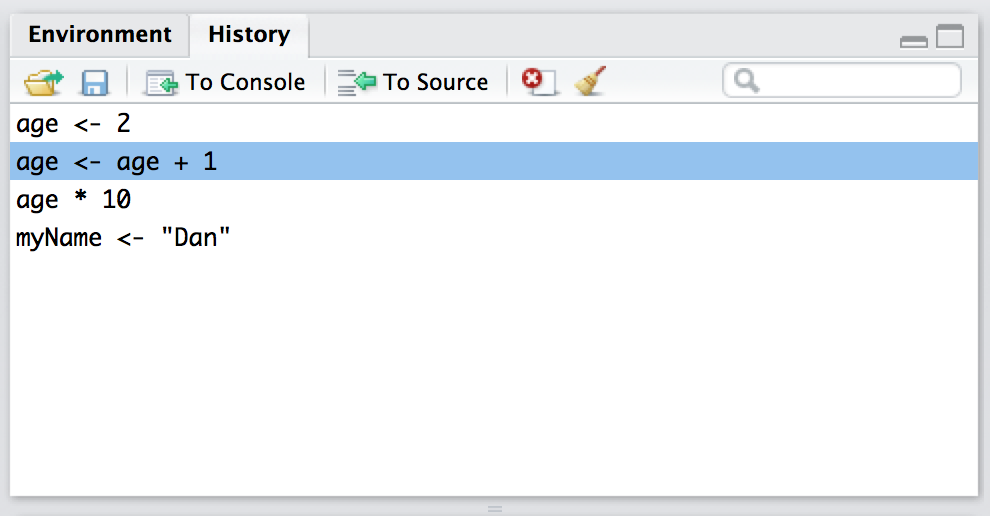
\includegraphics{/Users/dave/Documents/GitHub/stats-remix-advanced/bookdown/img/introR/historyTab.png}
\caption{\label{fig:RStudiohistory}The history panel is located in the top right hand side of the RStudio window. Click on the word ``History'' and it displays this panel.}
\end{figure}

\hypertarget{vectors}{%
\section{Storing many numbers as a vector}\label{vectors}}

At this point we've covered functions in enough detail to get us safely through the next couple of chapters (with one small exception: see Section \ref{generics}, so let's return to our discussion of variables. When I introduced variables in Section \ref{assign} I showed you how we can use variables to store a single number. In this section, we'll extend this idea and look at how to store multiple numbers within the one variable. In R, the name for a variable that can store multiple values is a \textbf{\emph{vector}}. So let's create one.

\hypertarget{creating-a-vector}{%
\subsection{Creating a vector}\label{creating-a-vector}}

Let's stick to my silly ``get rich quick by textbook writing'' example. Suppose the textbook company (if I actually had one, that is) sends me sales data on a monthly basis. Since my class start in late February, we might expect most of the sales to occur towards the start of the year. Let's suppose that I have 100 sales in February, 200 sales in March and 50 sales in April, and no other sales for the rest of the year. What I would like to do is have a variable -- let's call it \texttt{sales.by.month} -- that stores all this sales data. The first number stored should be \texttt{0} since I had no sales in January, the second should be \texttt{100}, and so on. The simplest way to do this in R is to use the \textbf{\emph{combine}} function, \texttt{c()}. To do so, all we have to do is type all the numbers you want to store in a comma separated list, like this:\footnote{Notice that I didn't specify any argument names here. The \texttt{c()} function is one of those cases where we don't use names. We just type all the numbers, and R just dumps them all in a single variable.}

\begin{Shaded}
\begin{Highlighting}[]
\NormalTok{sales.by.month }\OtherTok{\textless{}{-}} \FunctionTok{c}\NormalTok{(}\DecValTok{0}\NormalTok{, }\DecValTok{100}\NormalTok{, }\DecValTok{200}\NormalTok{, }\DecValTok{50}\NormalTok{, }\DecValTok{0}\NormalTok{, }\DecValTok{0}\NormalTok{, }\DecValTok{0}\NormalTok{, }\DecValTok{0}\NormalTok{, }\DecValTok{0}\NormalTok{, }\DecValTok{0}\NormalTok{, }\DecValTok{0}\NormalTok{, }\DecValTok{0}\NormalTok{)}
\NormalTok{sales.by.month}
\end{Highlighting}
\end{Shaded}

\begin{verbatim}
##  [1]   0 100 200  50   0   0   0   0   0   0   0   0
\end{verbatim}

To use the correct terminology here, we have a single variable here called \texttt{sales.by.month}: this variable is a vector that consists of 12 \textbf{\emph{elements}}.

\hypertarget{a-handy-digression}{%
\subsection{A handy digression}\label{a-handy-digression}}

Now that we've learned how to put information into a vector, the next thing to understand is how to pull that information back out again. However, before I do so it's worth taking a slight detour. If you've been following along, typing all the commands into R yourself, it's possible that the output that you saw when we printed out the \texttt{sales.by.month} vector was slightly different to what I showed above. This would have happened if the window (or the RStudio panel) that contains the R console is really, really narrow. If that were the case, you might have seen output that looks something like this:

\begin{Shaded}
\begin{Highlighting}[]
\NormalTok{sales.by.month}
\end{Highlighting}
\end{Shaded}

\begin{verbatim}
##  [1]   0 100 200  50
##  [5]   0   0   0   0
##  [9]   0   0   0   0
\end{verbatim}

Because there wasn't much room on the screen, R has printed out the results over three lines. But that's not the important thing to notice. The important point is that the first line has a \texttt{{[}1{]}} in front of it, whereas the second line starts with \texttt{{[}5{]}} and the third with \texttt{{[}9{]}}. It's pretty clear what's happening here. For the first row, R has printed out the 1st element through to the 4th element, so it starts that row with a \texttt{{[}1{]}}. For the second row, R has printed out the 5th element of the vector through to the 8th one, and so it begins that row with a \texttt{{[}5{]}} so that you can tell where it's up to at a glance. It might seem a bit odd to you that R does this, but in some ways it's a kindness, especially when dealing with larger data sets!

\hypertarget{vectorsubset}{%
\subsection{Getting information out of vectors}\label{vectorsubset}}

To get back to the main story, let's consider the problem of how to get information out of a vector. At this point, you might have a sneaking suspicion that the answer has something to do with the \texttt{{[}1{]}} and \texttt{{[}9{]}} things that R has been printing out. And of course you are correct. Suppose I want to pull out the February sales data only. February is the second month of the year, so let's try this:

\begin{Shaded}
\begin{Highlighting}[]
\NormalTok{sales.by.month[}\DecValTok{2}\NormalTok{]}
\end{Highlighting}
\end{Shaded}

\begin{verbatim}
## [1] 100
\end{verbatim}

Yep, that's the February sales all right. But there's a subtle detail to be aware of here: notice that R outputs \texttt{{[}1{]}\ 100}, \emph{not} \texttt{{[}2{]}\ 100}. This is because R is being extremely literal. When we typed in \texttt{sales.by.month{[}2{]}}, we asked R to find exactly \emph{one} thing, and that one thing happens to be the second element of our \texttt{sales.by.month} vector. So, when it outputs \texttt{{[}1{]}\ 100} what R is saying is that the first number \emph{that we just asked for} is \texttt{100}. This behaviour makes more sense when you realise that we can use this trick to create new variables. For example, I could create a \texttt{february.sales} variable like this:

\begin{Shaded}
\begin{Highlighting}[]
\NormalTok{february.sales }\OtherTok{\textless{}{-}}\NormalTok{ sales.by.month[}\DecValTok{2}\NormalTok{]}
\NormalTok{february.sales}
\end{Highlighting}
\end{Shaded}

\begin{verbatim}
## [1] 100
\end{verbatim}

Obviously, the new variable \texttt{february.sales} should only have one element and so when I print it out this new variable, the R output begins with a \texttt{{[}1{]}} because \texttt{100} is the value of the first (and only) element of \texttt{february.sales}. The fact that this also happens to be the value of the second element of \texttt{sales.by.month} is irrelevant. We'll pick this topic up again shortly (Section \ref{indexing}).

\hypertarget{altering-the-elements-of-a-vector}{%
\subsection{Altering the elements of a vector}\label{altering-the-elements-of-a-vector}}

Sometimes you'll want to change the values stored in a vector. Imagine my surprise when the publisher rings me up to tell me that the sales data for May are wrong. There were actually an additional 25 books sold in May, but there was an error or something so they hadn't told me about it. How can I fix my \texttt{sales.by.month} variable? One possibility would be to assign the whole vector again from the beginning, using \texttt{c()}. But that's a lot of typing. Also, it's a little wasteful: why should R have to redefine the sales figures for all 12 months, when only the 5th one is wrong? Fortunately, we can tell R to change only the 5th element, using this trick:

\begin{Shaded}
\begin{Highlighting}[]
\NormalTok{sales.by.month[}\DecValTok{5}\NormalTok{] }\OtherTok{\textless{}{-}} \DecValTok{25}
\NormalTok{sales.by.month}
\end{Highlighting}
\end{Shaded}

\begin{verbatim}
##  [1]   0 100 200  50  25   0   0   0   0   0   0   0
\end{verbatim}

Another way to edit variables is to use the \texttt{edit()} or \texttt{fix()} functions. I won't discuss them in detail right now, but you can check them out on your own.

\hypertarget{veclength}{%
\subsection{Useful things to know about vectors}\label{veclength}}

Before moving on, I want to mention a couple of other things about vectors. Firstly, you often find yourself wanting to know how many elements there are in a vector (usually because you've forgotten). You can use the \texttt{length()} function to do this. It's quite straightforward:

\begin{Shaded}
\begin{Highlighting}[]
\FunctionTok{length}\NormalTok{( }\AttributeTok{x =}\NormalTok{ sales.by.month )}
\end{Highlighting}
\end{Shaded}

\begin{verbatim}
## [1] 12
\end{verbatim}

Secondly, you often want to alter all of the elements of a vector at once. For instance, suppose I wanted to figure out how much money I made in each month. Since I'm earning an exciting \$7 per book (no seriously, that's actually pretty close to what authors get on the very expensive textbooks that you're expected to purchase), what I want to do is multiply each element in the \texttt{sales.by.month} vector by \texttt{7}. R makes this pretty easy, as the following example shows:

\begin{Shaded}
\begin{Highlighting}[]
\NormalTok{sales.by.month }\SpecialCharTok{*} \DecValTok{7}
\end{Highlighting}
\end{Shaded}

\begin{verbatim}
##  [1]    0  700 1400  350  175    0    0    0    0    0    0    0
\end{verbatim}

In other words, when you multiply a vector by a single number, all elements in the vector get multiplied. The same is true for addition, subtraction, division and taking powers. So that's neat. On the other hand, suppose I wanted to know how much money I was making per day, rather than per month. Since not every month has the same number of days, I need to do something slightly different. Firstly, I'll create two new vectors:

\begin{Shaded}
\begin{Highlighting}[]
\NormalTok{days.per.month }\OtherTok{\textless{}{-}} \FunctionTok{c}\NormalTok{(}\DecValTok{31}\NormalTok{, }\DecValTok{28}\NormalTok{, }\DecValTok{31}\NormalTok{, }\DecValTok{30}\NormalTok{, }\DecValTok{31}\NormalTok{, }\DecValTok{30}\NormalTok{, }\DecValTok{31}\NormalTok{, }\DecValTok{31}\NormalTok{, }\DecValTok{30}\NormalTok{, }\DecValTok{31}\NormalTok{, }\DecValTok{30}\NormalTok{, }\DecValTok{31}\NormalTok{)}
\NormalTok{profit }\OtherTok{\textless{}{-}}\NormalTok{ sales.by.month }\SpecialCharTok{*} \DecValTok{7}
\end{Highlighting}
\end{Shaded}

Obviously, the \texttt{profit} variable is the same one we created earlier, and the \texttt{days.per.month} variable is pretty straightforward. What I want to do is divide every element of \texttt{profit} by the \emph{corresponding} element of \texttt{days.per.month}. Again, R makes this pretty easy:

\begin{Shaded}
\begin{Highlighting}[]
\NormalTok{profit }\SpecialCharTok{/}\NormalTok{ days.per.month}
\end{Highlighting}
\end{Shaded}

\begin{verbatim}
##  [1]  0.000000 25.000000 45.161290 11.666667  5.645161  0.000000  0.000000
##  [8]  0.000000  0.000000  0.000000  0.000000  0.000000
\end{verbatim}

I still don't like all those zeros, but that's not what matters here. Notice that the second element of the output is 25, because R has divided the second element of \texttt{profit} (i.e.~700) by the second element of \texttt{days.per.month} (i.e.~28). Similarly, the third element of the output is equal to 1400 divided by 31, and so on. We'll talk more about calculations involving vectors later on (and in particular a thing called the ``recycling rule''; Section \ref{recycling}), but that's enough detail for now.

\hypertarget{text}{%
\section{Storing text data}\label{text}}

A lot of the time your data will be numeric in nature, but not always. Sometimes your data really needs to be described using text, not using numbers. To address this, we need to consider the situation where our variables store text. To create a variable that stores the word ``hello'', we can type this:

\begin{Shaded}
\begin{Highlighting}[]
\NormalTok{greeting }\OtherTok{\textless{}{-}} \StringTok{"hello"}
\NormalTok{greeting}
\end{Highlighting}
\end{Shaded}

\begin{verbatim}
## [1] "hello"
\end{verbatim}

When interpreting this, it's important to recognise that the quote marks here \emph{aren't} part of the string itself. They're just something that we use to make sure that R knows to treat the characters that they enclose as a piece of text data, known as a \textbf{\emph{character string}}. In other words, R treats \texttt{"hello"} as a string containing the word ``hello''; but if I had typed \texttt{hello} instead, R would go looking for a variable by that name! You can also use \texttt{\textquotesingle{}hello\textquotesingle{}} to specify a character string.

Okay, so that's how we store the text. Next, it's important to recognise that when we do this, R stores the entire word \texttt{"hello"} as a \emph{single} element: our \texttt{greeting} variable is \emph{not} a vector of five different letters. Rather, it has only the one element, and that element corresponds to the entire character string \texttt{"hello"}. To illustrate this, if I actually ask R to find the first element of \texttt{greeting}, it prints the whole string:

\begin{Shaded}
\begin{Highlighting}[]
\NormalTok{greeting[}\DecValTok{1}\NormalTok{]}
\end{Highlighting}
\end{Shaded}

\begin{verbatim}
## [1] "hello"
\end{verbatim}

Of course, there's no reason why I can't create a vector of character strings. For instance, if we were to continue with the example of my attempts to look at the monthly sales data for my book, one variable I might want would include the names of all 12 \texttt{months}.\footnote{Though actually there's no real need to do this, since R has an inbuilt variable called \texttt{month.name} that you can use for this purpose.} To do so, I could type in a command like this

\begin{Shaded}
\begin{Highlighting}[]
\NormalTok{months }\OtherTok{\textless{}{-}} \FunctionTok{c}\NormalTok{(}\StringTok{"January"}\NormalTok{, }\StringTok{"February"}\NormalTok{, }\StringTok{"March"}\NormalTok{, }\StringTok{"April"}\NormalTok{, }\StringTok{"May"}\NormalTok{, }\StringTok{"June"}\NormalTok{,}
            \StringTok{"July"}\NormalTok{, }\StringTok{"August"}\NormalTok{, }\StringTok{"September"}\NormalTok{, }\StringTok{"October"}\NormalTok{, }\StringTok{"November"}\NormalTok{, }
            \StringTok{"December"}\NormalTok{)}
\end{Highlighting}
\end{Shaded}

This is a \textbf{\emph{character vector}} containing 12 elements, each of which is the name of a month. So if I wanted R to tell me the name of the fourth month, all I would do is this:

\begin{Shaded}
\begin{Highlighting}[]
\NormalTok{months[}\DecValTok{4}\NormalTok{]}
\end{Highlighting}
\end{Shaded}

\begin{verbatim}
## [1] "April"
\end{verbatim}

\hypertarget{simpletext}{%
\subsection{Working with text}\label{simpletext}}

Working with text data is somewhat more complicated than working with numeric data, and I discuss some of the basic ideas in Section \ref{textprocessing}, but for purposes of the current chapter we only need this bare bones sketch. The only other thing I want to do before moving on is show you an example of a function that can be applied to text data. So far, most of the functions that we have seen (i.e., \texttt{sqrt()}, \texttt{abs()} and \texttt{round()}) only make sense when applied to numeric data (e.g., you can't calculate the square root of ``hello''), and we've seen one function that can be applied to pretty much any variable or vector (i.e., \texttt{length()}). So it might be nice to see an example of a function that can be applied to text.

The function I'm going to introduce you to is called \texttt{nchar()}, and what it does is count the number of individual characters that make up a string. Recall earlier that when we tried to calculate the \texttt{length()} of our \texttt{greeting} variable it returned a value of \texttt{1}: the \texttt{greeting} variable contains only the one string, which happens to be \texttt{"hello"}. But what if I want to know how many letters there are in the word? Sure, I could \emph{count} them, but that's boring, and more to the point it's a terrible strategy if what I wanted to know was the number of letters in \emph{War and Peace}. That's where the \texttt{nchar()} function is helpful:

\begin{Shaded}
\begin{Highlighting}[]
\FunctionTok{nchar}\NormalTok{( }\AttributeTok{x =}\NormalTok{ greeting )}
\end{Highlighting}
\end{Shaded}

\begin{verbatim}
## [1] 5
\end{verbatim}

That makes sense, since there are in fact 5 letters in the string \texttt{"hello"}. Better yet, you can apply \texttt{nchar()} to whole vectors. So, for instance, if I want R to tell me how many letters there are in the names of each of the 12 months, I can do this:

\begin{Shaded}
\begin{Highlighting}[]
\FunctionTok{nchar}\NormalTok{( }\AttributeTok{x =}\NormalTok{ months )}
\end{Highlighting}
\end{Shaded}

\begin{verbatim}
##  [1] 7 8 5 5 3 4 4 6 9 7 8 8
\end{verbatim}

So that's nice to know. The \texttt{nchar()} function can do a bit more than this, and there's a lot of other functions that you can do to extract more information from text or do all sorts of fancy things. However, the goal here is not to teach any of that! The goal right now is just to see an example of a function that actually does work when applied to text.

\hypertarget{logicals}{%
\section{Storing ``true or false'' data}\label{logicals}}

Time to move onto a third kind of data. A key concept in that a lot of R relies on is the idea of a \textbf{\emph{logical value}}. A logical value is an assertion about whether something is true or false. This is implemented in R in a pretty straightforward way. There are two logical values, namely \texttt{TRUE} and \texttt{FALSE}. Despite the simplicity, a logical values are very useful things. Let's see how they work.

\hypertarget{assessing-mathematical-truths}{%
\subsection{Assessing mathematical truths}\label{assessing-mathematical-truths}}

In George Orwell's classic book \emph{1984}, one of the slogans used by the totalitarian Party was ``two plus two equals five'', the idea being that the political domination of human freedom becomes complete when it is possible to subvert even the most basic of truths. It's a terrifying thought, especially when the protagonist Winston Smith finally breaks down under torture and agrees to the proposition. ``Man is infinitely malleable'', the book says. I'm pretty sure that this isn't true of humans\footnote{I offer up my teenage attempts to be ``cool'' as evidence that some things just can't be done.} but it's definitely not true of R. R is not infinitely malleable. It has rather firm opinions on the topic of what is and isn't true, at least as regards basic mathematics. If I ask it to calculate \texttt{2\ +\ 2}, it always gives the same answer, and it's not bloody 5:

\begin{Shaded}
\begin{Highlighting}[]
\DecValTok{2} \SpecialCharTok{+} \DecValTok{2}
\end{Highlighting}
\end{Shaded}

\begin{verbatim}
## [1] 4
\end{verbatim}

Of course, so far R is just doing the calculations. I haven't asked it to explicitly assert that \(2+2 = 4\) is a true statement. If I want R to make an explicit judgement, I can use a command like this:

\begin{Shaded}
\begin{Highlighting}[]
\DecValTok{2} \SpecialCharTok{+} \DecValTok{2} \SpecialCharTok{==} \DecValTok{4}
\end{Highlighting}
\end{Shaded}

\begin{verbatim}
## [1] TRUE
\end{verbatim}

What I've done here is use the \textbf{\emph{equality operator}}, \texttt{==}, to force R to make a ``true or false'' judgement.\footnote{Note that this is a very different operator to the assignment operator \texttt{=} that I talked about in Section \ref{assign}. A common typo that people make when trying to write logical commands in R (or other languages, since the ``\texttt{=} versus \texttt{==}'' distinction is important in most programming languages) is to accidentally type \texttt{=} when you really mean \texttt{==}. Be especially cautious with this -- I've been programming in various languages since I was a teenager, and I \emph{still} screw this up a lot. Hm. I think I see why I wasn't cool as a teenager. And why I'm still not cool.} Okay, let's see what R thinks of the Party slogan:

\begin{Shaded}
\begin{Highlighting}[]
\DecValTok{2}\SpecialCharTok{+}\DecValTok{2} \SpecialCharTok{==} \DecValTok{5}
\end{Highlighting}
\end{Shaded}

\begin{verbatim}
## [1] FALSE
\end{verbatim}

Booyah! Freedom and ponies for all! Or something like that. Anyway, it's worth having a look at what happens if I try to \emph{force} R to believe that two plus two is five by making an assignment statement like \texttt{2\ +\ 2\ =\ 5} or \texttt{2\ +\ 2\ \textless{}-\ 5}. When I do this, here's what happens:

\begin{Shaded}
\begin{Highlighting}[]
\DecValTok{2} \SpecialCharTok{+} \DecValTok{2} \OtherTok{=} \DecValTok{5}
\end{Highlighting}
\end{Shaded}

\begin{verbatim}
## Error in 2 + 2 = 5: target of assignment expands to non-language object
\end{verbatim}

R doesn't like this very much. It recognises that \texttt{2\ +\ 2} is \emph{not} a variable (that's what the ``non-language object'' part is saying), and it won't let you try to ``reassign'' it. While R is pretty flexible, and actually does let you do some quite remarkable things to redefine parts of R itself, there are just some basic, primitive truths that it refuses to give up. It won't change the laws of addition, and it won't change the definition of the number \texttt{2}.

That's probably for the best.

\hypertarget{logical-operations}{%
\subsection{Logical operations}\label{logical-operations}}

So now we've seen logical operations at work, but so far we've only seen the simplest possible example. You probably won't be surprised to discover that we can combine logical operations with other operations and functions in a more complicated way, like this:

\begin{Shaded}
\begin{Highlighting}[]
\DecValTok{3}\SpecialCharTok{*}\DecValTok{3} \SpecialCharTok{+} \DecValTok{4}\SpecialCharTok{*}\DecValTok{4} \SpecialCharTok{==} \DecValTok{5}\SpecialCharTok{*}\DecValTok{5}
\end{Highlighting}
\end{Shaded}

\begin{verbatim}
## [1] TRUE
\end{verbatim}

or this

\begin{Shaded}
\begin{Highlighting}[]
\FunctionTok{sqrt}\NormalTok{( }\DecValTok{25}\NormalTok{ ) }\SpecialCharTok{==} \DecValTok{5}
\end{Highlighting}
\end{Shaded}

\begin{verbatim}
## [1] TRUE
\end{verbatim}

Not only that, but as Table \ref{tab:logicals} illustrates, there are several other logical operators that you can use, corresponding to some basic mathematical concepts.

\begin{table}

\caption{\label{tab:logicals}Some logical operators. Technically I should be calling these "binary relational operators", but quite frankly I don't want to. It's my book so no-one can make me.}
\centering
\begin{tabular}[t]{llll}
\toprule
operation & operator & example input & answer\\
\midrule
less than & < & 2 < 3 & `TRUE`\\
less than or equal to & <= & 2 <= 2 & `TRUE`\\
greater than & > & 2 > 3 & `FALSE`\\
greater than or equal to & >= & 2 >= 2 & `TRUE`\\
equal to & == & 2 == 3 & `FALSE`\\
\addlinespace
not equal to & != & 2 != 3 & `TRUE`\\
\bottomrule
\end{tabular}
\end{table}

Hopefully these are all pretty self-explanatory: for example, the \textbf{\emph{less than}} operator \texttt{\textless{}} checks to see if the number on the left is less than the number on the right. If it's less, then R returns an answer of \texttt{TRUE}:

\begin{Shaded}
\begin{Highlighting}[]
\DecValTok{99} \SpecialCharTok{\textless{}} \DecValTok{100}
\end{Highlighting}
\end{Shaded}

\begin{verbatim}
## [1] TRUE
\end{verbatim}

but if the two numbers are equal, or if the one on the right is larger, then R returns an answer of \texttt{FALSE}, as the following two examples illustrate:

\begin{Shaded}
\begin{Highlighting}[]
\DecValTok{100} \SpecialCharTok{\textless{}} \DecValTok{100}
\end{Highlighting}
\end{Shaded}

\begin{verbatim}
## [1] FALSE
\end{verbatim}

\begin{Shaded}
\begin{Highlighting}[]
\DecValTok{100} \SpecialCharTok{\textless{}} \DecValTok{99}
\end{Highlighting}
\end{Shaded}

\begin{verbatim}
## [1] FALSE
\end{verbatim}

In contrast, the \textbf{\emph{less than or equal to}} operator \texttt{\textless{}=} will do exactly what it says. It returns a value of \texttt{TRUE} if the number of the left hand side is less than or equal to the number on the right hand side. So if we repeat the previous two examples using \texttt{\textless{}=}, here's what we get:

\begin{Shaded}
\begin{Highlighting}[]
\DecValTok{100} \SpecialCharTok{\textless{}=} \DecValTok{100}
\end{Highlighting}
\end{Shaded}

\begin{verbatim}
## [1] TRUE
\end{verbatim}

\begin{Shaded}
\begin{Highlighting}[]
\DecValTok{100} \SpecialCharTok{\textless{}=} \DecValTok{99}
\end{Highlighting}
\end{Shaded}

\begin{verbatim}
## [1] FALSE
\end{verbatim}

And at this point I hope it's pretty obvious what the \textbf{\emph{greater than}} operator \texttt{\textgreater{}} and the \textbf{\emph{greater than or equal to}} operator \texttt{\textgreater{}=} do! Next on the list of logical operators is the \textbf{\emph{not equal to}} operator \texttt{!=} which -- as with all the others -- does what it says it does. It returns a value of \texttt{TRUE} when things on either side are not identical to each other. Therefore, since \(2+2\) isn't equal to \(5\), we get:

\begin{Shaded}
\begin{Highlighting}[]
\DecValTok{2} \SpecialCharTok{+} \DecValTok{2} \SpecialCharTok{!=} \DecValTok{5}
\end{Highlighting}
\end{Shaded}

\begin{verbatim}
## [1] TRUE
\end{verbatim}

We're not quite done yet. There are three more logical operations that are worth knowing about, listed in Table \ref{tab:logicals2}.

\begin{table}

\caption{\label{tab:logicals2}Some more logical operators.}
\centering
\begin{tabular}[t]{llll}
\toprule
operation & operator & example input & answer\\
\midrule
not & ! & !(1==1) & `FALSE`\\
or & | & (1==1) | (2==3) & `TRUE`\\
and & \& & (1==1) \& (2==3) & `FALSE`\\
\bottomrule
\end{tabular}
\end{table}

These are the \textbf{\emph{not}} operator \texttt{!}, the \textbf{\emph{and}} operator \texttt{\&}, and the \textbf{\emph{or}} operator \texttt{\textbar{}}. Like the other logical operators, their behaviour is more or less exactly what you'd expect given their names. For instance, if I ask you to assess the claim that ``either \(2+2 = 4\) \emph{or} \(2+2 = 5\)'' you'd say that it's true. Since it's an ``either-or'' statement, all we need is for one of the two parts to be true. That's what the \texttt{\textbar{}} operator does:

\begin{Shaded}
\begin{Highlighting}[]
\NormalTok{(}\DecValTok{2}\SpecialCharTok{+}\DecValTok{2} \SpecialCharTok{==} \DecValTok{4}\NormalTok{) }\SpecialCharTok{|}\NormalTok{ (}\DecValTok{2}\SpecialCharTok{+}\DecValTok{2} \SpecialCharTok{==} \DecValTok{5}\NormalTok{)}
\end{Highlighting}
\end{Shaded}

\begin{verbatim}
## [1] TRUE
\end{verbatim}

On the other hand, if I ask you to assess the claim that ``both \(2+2 = 4\) \emph{and} \(2+2 = 5\)'' you'd say that it's false. Since this is an \emph{and} statement we need both parts to be true. And that's what the \texttt{\&} operator does:

\begin{Shaded}
\begin{Highlighting}[]
\NormalTok{(}\DecValTok{2}\SpecialCharTok{+}\DecValTok{2} \SpecialCharTok{==} \DecValTok{4}\NormalTok{) }\SpecialCharTok{\&}\NormalTok{ (}\DecValTok{2}\SpecialCharTok{+}\DecValTok{2} \SpecialCharTok{==} \DecValTok{5}\NormalTok{)}
\end{Highlighting}
\end{Shaded}

\begin{verbatim}
## [1] FALSE
\end{verbatim}

Finally, there's the \emph{not} operator, which is simple but annoying to describe in English. If I ask you to assess my claim that ``it is not true that \(2+2 = 5\)'' then you would say that my claim is true; because my claim is that ``\(2+2 = 5\) is false''. And I'm right. If we write this as an R command we get this:

\begin{Shaded}
\begin{Highlighting}[]
\SpecialCharTok{!}\NormalTok{ (}\DecValTok{2}\SpecialCharTok{+}\DecValTok{2} \SpecialCharTok{==} \DecValTok{5}\NormalTok{)}
\end{Highlighting}
\end{Shaded}

\begin{verbatim}
## [1] TRUE
\end{verbatim}

In other words, since \texttt{2+2\ ==\ 5} is a \texttt{FALSE} statement, it must be the case that \texttt{!(2+2\ ==\ 5)} is a \texttt{TRUE} one. Essentially, what we've really done is claim that ``not false'' is the same thing as ``true''. Obviously, this isn't really quite right in real life. But R lives in a much more black or white world: for R everything is either true or false. No shades of gray are allowed. We can actually see this much more explicitly, like this:

\begin{Shaded}
\begin{Highlighting}[]
\SpecialCharTok{!} \ConstantTok{FALSE}
\end{Highlighting}
\end{Shaded}

\begin{verbatim}
## [1] TRUE
\end{verbatim}

Of course, in our \(2+2 = 5\) example, we didn't really need to use ``not'' \texttt{!} and ``equals to'' \texttt{==} as two separate operators. We could have just used the ``not equals to'' operator \texttt{!=} like this:

\begin{Shaded}
\begin{Highlighting}[]
\DecValTok{2}\SpecialCharTok{+}\DecValTok{2} \SpecialCharTok{!=} \DecValTok{5}
\end{Highlighting}
\end{Shaded}

\begin{verbatim}
## [1] TRUE
\end{verbatim}

But there are many situations where you really do need to use the \texttt{!} operator. We'll see some later on.\footnote{A note for those of you who have taken a computer science class: yes, R does have a function for exclusive-or, namely \texttt{xor()}. Also worth noting is the fact that R makes the distinction between element-wise operators \texttt{\&} and \texttt{\textbar{}} and operators that look only at the first element of the vector, namely \texttt{\&\&} and \texttt{\textbar{}\textbar{}}. To see the distinction, compare the behaviour of a command like \texttt{c(FALSE,TRUE)\ \&\ c(TRUE,TRUE)} to the behaviour of something like \texttt{c(FALSE,TRUE)\ \&\&\ c(TRUE,TRUE)}. If this doesn't mean anything to you, ignore this footnote entirely. It's not important for the content of this book.}

\hypertarget{storing-and-using-logical-data}{%
\subsection{Storing and using logical data}\label{storing-and-using-logical-data}}

Up to this point, I've introduced \emph{numeric data} (in Sections \ref{assign} and \ref{vectors}) and \emph{character data} (in Section \ref{text}). So you might not be surprised to discover that these \texttt{TRUE} and \texttt{FALSE} values that R has been producing are actually a third kind of data, called \emph{logical data}. That is, when I asked R if \texttt{2\ +\ 2\ ==\ 5} and it said \texttt{{[}1{]}\ FALSE} in reply, it was actually producing information that we can store in variables. For instance, I could create a variable called \texttt{is.the.Party.correct}, which would store R's opinion:

\begin{Shaded}
\begin{Highlighting}[]
\NormalTok{is.the.Party.correct }\OtherTok{\textless{}{-}} \DecValTok{2} \SpecialCharTok{+} \DecValTok{2} \SpecialCharTok{==} \DecValTok{5}
\NormalTok{is.the.Party.correct}
\end{Highlighting}
\end{Shaded}

\begin{verbatim}
## [1] FALSE
\end{verbatim}

Alternatively, you can assign the value directly, by typing \texttt{TRUE} or \texttt{FALSE} in your command. Like this:

\begin{Shaded}
\begin{Highlighting}[]
\NormalTok{is.the.Party.correct }\OtherTok{\textless{}{-}} \ConstantTok{FALSE}
\NormalTok{is.the.Party.correct}
\end{Highlighting}
\end{Shaded}

\begin{verbatim}
## [1] FALSE
\end{verbatim}

Better yet, because it's kind of tedious to type \texttt{TRUE} or \texttt{FALSE} over and over again, R provides you with a shortcut: you can use \texttt{T} and \texttt{F} instead (but it's case sensitive: \texttt{t} and \texttt{f} won't work).\footnote{Warning! \texttt{TRUE} and \texttt{FALSE} are reserved keywords in R, so you can trust that they always mean what they say they do. Unfortunately, the shortcut versions \texttt{T} and \texttt{F} do not have this property. It's even possible to create variables that set up the reverse meanings, by typing commands like \texttt{T\ \textless{}-\ FALSE} and \texttt{F\ \textless{}-\ TRUE}. This is kind of insane, and something that is generally thought to be a design flaw in R. Anyway, the long and short of it is that it's safer to use \texttt{TRUE} and \texttt{FALSE}.} So this works:

\begin{Shaded}
\begin{Highlighting}[]
\NormalTok{is.the.Party.correct }\OtherTok{\textless{}{-}}\NormalTok{ F}
\NormalTok{is.the.Party.correct}
\end{Highlighting}
\end{Shaded}

\begin{verbatim}
## [1] FALSE
\end{verbatim}

but this doesn't:

\begin{Shaded}
\begin{Highlighting}[]
\NormalTok{is.the.Party.correct }\OtherTok{\textless{}{-}}\NormalTok{ f}
\end{Highlighting}
\end{Shaded}

\begin{verbatim}
## Error in eval(expr, envir, enclos): object 'f' not found
\end{verbatim}

\hypertarget{vectors-of-logicals}{%
\subsection{Vectors of logicals}\label{vectors-of-logicals}}

The next thing to mention is that you can store vectors of logical values in exactly the same way that you can store vectors of numbers (Section \ref{vectors}) and vectors of text data (Section \ref{text}). Again, we can define them directly via the \texttt{c()} function, like this:

\begin{Shaded}
\begin{Highlighting}[]
\NormalTok{x }\OtherTok{\textless{}{-}} \FunctionTok{c}\NormalTok{(}\ConstantTok{TRUE}\NormalTok{, }\ConstantTok{TRUE}\NormalTok{, }\ConstantTok{FALSE}\NormalTok{)}
\NormalTok{x}
\end{Highlighting}
\end{Shaded}

\begin{verbatim}
## [1]  TRUE  TRUE FALSE
\end{verbatim}

or you can produce a vector of logicals by applying a logical operator to a vector. This might not make a lot of sense to you, so let's unpack it slowly. First, let's suppose we have a vector of numbers (i.e., a ``non-logical vector''). For instance, we could use the \texttt{sales.by.month} vector that we were using in Section \ref{vectors}. Suppose I wanted R to tell me, for each month of the year, whether I actually sold a book in that month. I can do that by typing this:

\begin{Shaded}
\begin{Highlighting}[]
\NormalTok{sales.by.month }\SpecialCharTok{\textgreater{}} \DecValTok{0}
\end{Highlighting}
\end{Shaded}

\begin{verbatim}
##  [1] FALSE  TRUE  TRUE  TRUE  TRUE FALSE FALSE FALSE FALSE FALSE FALSE
## [12] FALSE
\end{verbatim}

and again, I can store this in a vector if I want, as the example below illustrates:

\begin{Shaded}
\begin{Highlighting}[]
\NormalTok{any.sales.this.month }\OtherTok{\textless{}{-}}\NormalTok{ sales.by.month }\SpecialCharTok{\textgreater{}} \DecValTok{0}
\NormalTok{any.sales.this.month}
\end{Highlighting}
\end{Shaded}

\begin{verbatim}
##  [1] FALSE  TRUE  TRUE  TRUE  TRUE FALSE FALSE FALSE FALSE FALSE FALSE
## [12] FALSE
\end{verbatim}

In other words, \texttt{any.sales.this.month} is a logical vector whose elements are \texttt{TRUE} only if the corresponding element of \texttt{sales.by.month} is greater than zero. For instance, since I sold zero books in January, the first element is \texttt{FALSE}.

\hypertarget{logictext}{%
\subsection{Applying logical operation to text}\label{logictext}}

In a moment (Section \ref{indexing}) I'll show you why these logical operations and logical vectors are so handy, but before I do so I want to very briefly point out that you can apply them to text as well as to logical data. It's just that we need to be a bit more careful in understanding how R interprets the different operations. In this section I'll talk about how the equal to operator \texttt{==} applies to text, since this is the most important one. Obviously, the not equal to operator \texttt{!=} gives the exact opposite answers to \texttt{==} so I'm implicitly talking about that one too, but I won't give specific commands showing the use of \texttt{!=}. As for the other operators, I'll defer a more detailed discussion of this topic to Section \ref{logictext2}.

Okay, let's see how it works. In one sense, it's very simple. For instance, I can ask R if the word \texttt{"cat"} is the same as the word \texttt{"dog"}, like this:

\begin{Shaded}
\begin{Highlighting}[]
\StringTok{"cat"} \SpecialCharTok{==} \StringTok{"dog"}
\end{Highlighting}
\end{Shaded}

\begin{verbatim}
## [1] FALSE
\end{verbatim}

That's pretty obvious, and it's good to know that even R can figure that out. Similarly, R does recognise that a \texttt{"cat"} is a \texttt{"cat"}:

\begin{Shaded}
\begin{Highlighting}[]
\StringTok{"cat"} \SpecialCharTok{==} \StringTok{"cat"}
\end{Highlighting}
\end{Shaded}

\begin{verbatim}
## [1] TRUE
\end{verbatim}

Again, that's exactly what we'd expect. However, what you need to keep in mind is that R is not at all tolerant when it comes to grammar and spacing. If two strings differ in any way whatsoever, R will say that they're not equal to each other, as the following examples indicate:

\begin{Shaded}
\begin{Highlighting}[]
\StringTok{" cat"} \SpecialCharTok{==} \StringTok{"cat"}
\end{Highlighting}
\end{Shaded}

\begin{verbatim}
## [1] FALSE
\end{verbatim}

\begin{Shaded}
\begin{Highlighting}[]
\StringTok{"cat"} \SpecialCharTok{==} \StringTok{"CAT"}
\end{Highlighting}
\end{Shaded}

\begin{verbatim}
## [1] FALSE
\end{verbatim}

\begin{Shaded}
\begin{Highlighting}[]
\StringTok{"cat"} \SpecialCharTok{==} \StringTok{"c a t"}
\end{Highlighting}
\end{Shaded}

\begin{verbatim}
## [1] FALSE
\end{verbatim}

\hypertarget{indexing}{%
\section{Indexing vectors}\label{indexing}}

One last thing to add before finishing up this chapter. So far, whenever I've had to get information out of a vector, all I've done is typed something like \texttt{months{[}4{]}}; and when I do this R prints out the fourth element of the \texttt{months} vector. In this section, I'll show you two additional tricks for getting information out of the vector.

\hypertarget{extracting-multiple-elements}{%
\subsection{Extracting multiple elements}\label{extracting-multiple-elements}}

One very useful thing we can do is pull out more than one element at a time. In the previous example, we only used a single number (i.e., \texttt{2}) to indicate which element we wanted. Alternatively, we can use a vector. So, suppose I wanted the data for February, March and April. What I could do is use the vector \texttt{c(2,3,4)} to indicate which elements I want R to pull out. That is, I'd type this:

\begin{Shaded}
\begin{Highlighting}[]
\NormalTok{sales.by.month[ }\FunctionTok{c}\NormalTok{(}\DecValTok{2}\NormalTok{,}\DecValTok{3}\NormalTok{,}\DecValTok{4}\NormalTok{) ]}
\end{Highlighting}
\end{Shaded}

\begin{verbatim}
## [1] 100 200  50
\end{verbatim}

Notice that the order matters here. If I asked for the data in the reverse order (i.e., April first, then March, then February) by using the vector \texttt{c(4,3,2)}, then R outputs the data in the reverse order:

\begin{Shaded}
\begin{Highlighting}[]
\NormalTok{sales.by.month[ }\FunctionTok{c}\NormalTok{(}\DecValTok{4}\NormalTok{,}\DecValTok{3}\NormalTok{,}\DecValTok{2}\NormalTok{) ]}
\end{Highlighting}
\end{Shaded}

\begin{verbatim}
## [1]  50 200 100
\end{verbatim}

A second thing to be aware of is that R provides you with handy shortcuts for very common situations. For instance, suppose that I wanted to extract everything from the 2nd month through to the 8th month. One way to do this is to do the same thing I did above, and use the vector \texttt{c(2,3,4,5,6,7,8)} to indicate the elements that I want. That works just fine

\begin{Shaded}
\begin{Highlighting}[]
\NormalTok{sales.by.month[ }\FunctionTok{c}\NormalTok{(}\DecValTok{2}\NormalTok{,}\DecValTok{3}\NormalTok{,}\DecValTok{4}\NormalTok{,}\DecValTok{5}\NormalTok{,}\DecValTok{6}\NormalTok{,}\DecValTok{7}\NormalTok{,}\DecValTok{8}\NormalTok{) ]}
\end{Highlighting}
\end{Shaded}

\begin{verbatim}
## [1] 100 200  50  25   0   0   0
\end{verbatim}

but it's kind of a lot of typing. To help make this easier, R lets you use \texttt{2:8} as shorthand for \texttt{c(2,3,4,5,6,7,8)}, which makes things a lot simpler. First, let's just check that this is true:

\begin{Shaded}
\begin{Highlighting}[]
\DecValTok{2}\SpecialCharTok{:}\DecValTok{8}
\end{Highlighting}
\end{Shaded}

\begin{verbatim}
## [1] 2 3 4 5 6 7 8
\end{verbatim}

Next, let's check that we can use the \texttt{2:8} shorthand as a way to pull out the 2nd through 8th elements of \texttt{sales.by.months}:

\begin{Shaded}
\begin{Highlighting}[]
\NormalTok{sales.by.month[}\DecValTok{2}\SpecialCharTok{:}\DecValTok{8}\NormalTok{]}
\end{Highlighting}
\end{Shaded}

\begin{verbatim}
## [1] 100 200  50  25   0   0   0
\end{verbatim}

So that's kind of neat.

\hypertarget{logical-indexing}{%
\subsection{Logical indexing}\label{logical-indexing}}

At this point, I can introduce an extremely useful tool called \textbf{\emph{logical indexing}}. In the last section, I created a logical vector \texttt{any.sales.this.month}, whose elements are \texttt{TRUE} for any month in which I sold at least one book, and \texttt{FALSE} for all the others. However, that big long list of \texttt{TRUE}s and \texttt{FALSE}s is a little bit hard to read, so what I'd like to do is to have R select the names of the \texttt{months} for which I sold any books. Earlier on, I created a vector \texttt{months} that contains the names of each of the months. This is where logical indexing is handy. What I need to do is this:

\begin{Shaded}
\begin{Highlighting}[]
\NormalTok{months[ sales.by.month }\SpecialCharTok{\textgreater{}} \DecValTok{0}\NormalTok{ ]}
\end{Highlighting}
\end{Shaded}

\begin{verbatim}
## [1] "February" "March"    "April"    "May"
\end{verbatim}

To understand what's happening here, it's helpful to notice that \texttt{sales.by.month\ \textgreater{}\ 0} is the same logical expression that we used to create the \texttt{any.sales.this.month} vector in the last section. In fact, I could have just done this:

\begin{Shaded}
\begin{Highlighting}[]
\NormalTok{months[ any.sales.this.month ]}
\end{Highlighting}
\end{Shaded}

\begin{verbatim}
## [1] "February" "March"    "April"    "May"
\end{verbatim}

and gotten exactly the same result. In order to figure out which elements of \texttt{months} to include in the output, what R does is look to see if the corresponding element in \texttt{any.sales.this.month} is \texttt{TRUE}. Thus, since element 1 of \texttt{any.sales.this.month} is \texttt{FALSE}, R does not include \texttt{"January"} as part of the output; but since element 2 of \texttt{any.sales.this.month} is \texttt{TRUE}, R does include \texttt{"February"} in the output. Note that there's no reason why I can't use the same trick to find the actual sales numbers for those months. The command to do that would just be this:

\begin{Shaded}
\begin{Highlighting}[]
\NormalTok{sales.by.month [ sales.by.month }\SpecialCharTok{\textgreater{}} \DecValTok{0}\NormalTok{ ]}
\end{Highlighting}
\end{Shaded}

\begin{verbatim}
## [1] 100 200  50  25
\end{verbatim}

In fact, we can do the same thing with text. Here's an example. Suppose that -- to continue the saga of the textbook sales -- I later find out that the bookshop only had sufficient stocks for a few months of the year. They tell me that early in the year they had \texttt{"high"} stocks, which then dropped to \texttt{"low"} levels, and in fact for one month they were \texttt{"out"} of copies of the book for a while before they were able to replenish them. Thus I might have a variable called \texttt{stock.levels} which looks like this:

\begin{Shaded}
\begin{Highlighting}[]
\NormalTok{stock.levels}\OtherTok{\textless{}{-}}\FunctionTok{c}\NormalTok{(}\StringTok{"high"}\NormalTok{, }\StringTok{"high"}\NormalTok{, }\StringTok{"low"}\NormalTok{, }\StringTok{"out"}\NormalTok{, }\StringTok{"out"}\NormalTok{, }\StringTok{"high"}\NormalTok{,}
                \StringTok{"high"}\NormalTok{, }\StringTok{"high"}\NormalTok{, }\StringTok{"high"}\NormalTok{, }\StringTok{"high"}\NormalTok{, }\StringTok{"high"}\NormalTok{, }\StringTok{"high"}\NormalTok{)}

\NormalTok{stock.levels}
\end{Highlighting}
\end{Shaded}

\begin{verbatim}
##  [1] "high" "high" "low"  "out"  "out"  "high" "high" "high" "high" "high"
## [11] "high" "high"
\end{verbatim}

Thus, if I want to know the months for which the bookshop was out of my book, I could apply the logical indexing trick, but with the character vector \texttt{stock.levels}, like this:

\begin{Shaded}
\begin{Highlighting}[]
\NormalTok{months[stock.levels }\SpecialCharTok{==} \StringTok{"out"}\NormalTok{]}
\end{Highlighting}
\end{Shaded}

\begin{verbatim}
## [1] "April" "May"
\end{verbatim}

Alternatively, if I want to know when the bookshop was either low on copies or out of copies, I could do this:

\begin{Shaded}
\begin{Highlighting}[]
\NormalTok{months[stock.levels }\SpecialCharTok{==} \StringTok{"out"} \SpecialCharTok{|}\NormalTok{ stock.levels }\SpecialCharTok{==} \StringTok{"low"}\NormalTok{]}
\end{Highlighting}
\end{Shaded}

\begin{verbatim}
## [1] "March" "April" "May"
\end{verbatim}

or this

\begin{Shaded}
\begin{Highlighting}[]
\NormalTok{months[stock.levels }\SpecialCharTok{!=} \StringTok{"high"}\NormalTok{ ]}
\end{Highlighting}
\end{Shaded}

\begin{verbatim}
## [1] "March" "April" "May"
\end{verbatim}

Either way, I get the answer I want.

At this point, I hope you can see why logical indexing is such a useful thing. It's a very basic, yet very powerful way to manipulate data. We'll talk a lot more about how to manipulate data in Chapter \ref{datahandling}, since it's a critical skill for real world research that is often overlooked in introductory research methods classes (or at least, that's been my experience). It does take a bit of practice to become completely comfortable using logical indexing, so it's a good idea to play around with these sorts of commands. Try creating a few different variables of your own, and then ask yourself questions like ``how do I get R to spit out all the elements that are {[}blah{]}''. Practice makes perfect, and it's only by practicing logical indexing that you'll perfect the art of yelling frustrated insults at your computer.\footnote{Well, I say that\ldots{} but in my personal experience it wasn't until I started learning ``regular expressions'' that my loathing of computers reached its peak.}

\hypertarget{quitting-r}{%
\section{Quitting R}\label{quitting-r}}

\begin{figure}
\centering
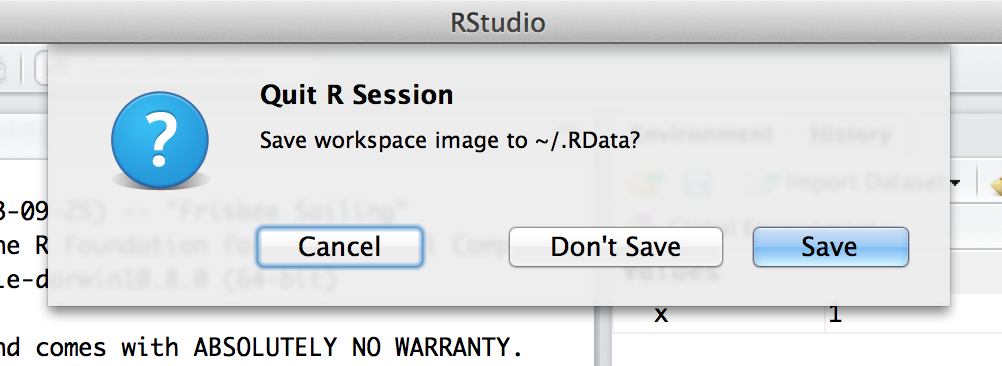
\includegraphics{/Users/dave/Documents/GitHub/stats-remix-advanced/bookdown/img/introR/Rstudio_quit.png}
\caption{\label{fig:quitR}The dialog box that shows up when you try to close RStudio.}
\end{figure}

There's one last thing I should cover in this chapter: how to quit R. When I say this, I'm not trying to imply that R is some kind of pathological addition and that you need to call the R QuitLine or wear patches to control the cravings (although you certainly might argue that there's something seriously pathological about being addicted to R). I just mean how to exit the program. Assuming you're running R in the usual way (i.e., through RStudio or the default GUI on a Windows or Mac computer), then you can just shut down the application in the normal way. However, R also has a function, called \texttt{q()} that you can use to quit, which is pretty handy if you're running R in a terminal window.

Regardless of what method you use to quit R, when you do so for the first time R will probably ask you if you want to save the ``workspace image''. We'll talk a lot more about loading and saving data in Section \ref{load}, but I figured we'd better quickly cover this now otherwise you're going to get annoyed when you close R at the end of the chapter. If you're using RStudio, you'll see a dialog box that looks like the one shown in Figure \ref{fig:quitR}. If you're using a text based interface you'll see this:

\begin{Shaded}
\begin{Highlighting}[]
\FunctionTok{q}\NormalTok{()}

\DocumentationTok{\#\# Save workspace image? [y/n/c]: }
\end{Highlighting}
\end{Shaded}

The \texttt{y/n/c} part here is short for ``yes / no / cancel''. Type \texttt{y} if you want to save, \texttt{n} if you don't, and \texttt{c} if you've changed your mind and you don't want to quit after all.

What does this actually \emph{mean}? What's going on is that R wants to know if you want to save all those variables that you've been creating, so that you can use them later. This sounds like a great idea, so it's really tempting to type \texttt{y} or click the ``Save'' button. To be honest though, I very rarely do this, and it kind of annoys me a little bit\ldots{} what R is \emph{really} asking is if you want it to store these variables in a ``default'' data file, which it will automatically reload for you next time you open R. And quite frankly, if I'd wanted to save the variables, then I'd have already saved them before trying to quit. Not only that, I'd have saved them to a location of \emph{my} choice, so that I can find it again later. So I personally never bother with this.

In fact, every time I install R on a new machine one of the first things I do is change the settings so that it never asks me again. You can do this in RStudio really easily: use the menu system to find the RStudio option; the dialog box that comes up will give you an option to tell R never to whine about this again (see Figure \ref{fig:RStudiooptions}. On a Mac, you can open this window by going to the ``RStudio'' menu and selecting ``Preferences''. On a Windows machine you go to the ``Tools'' menu and select ``Global Options''. Under the ``General'' tab you'll see an option that reads ``Save workspace to .Rdata on exit''. By default this is set to ``ask''. If you want R to stop asking, change it to ``never''.

\begin{figure}
\centering
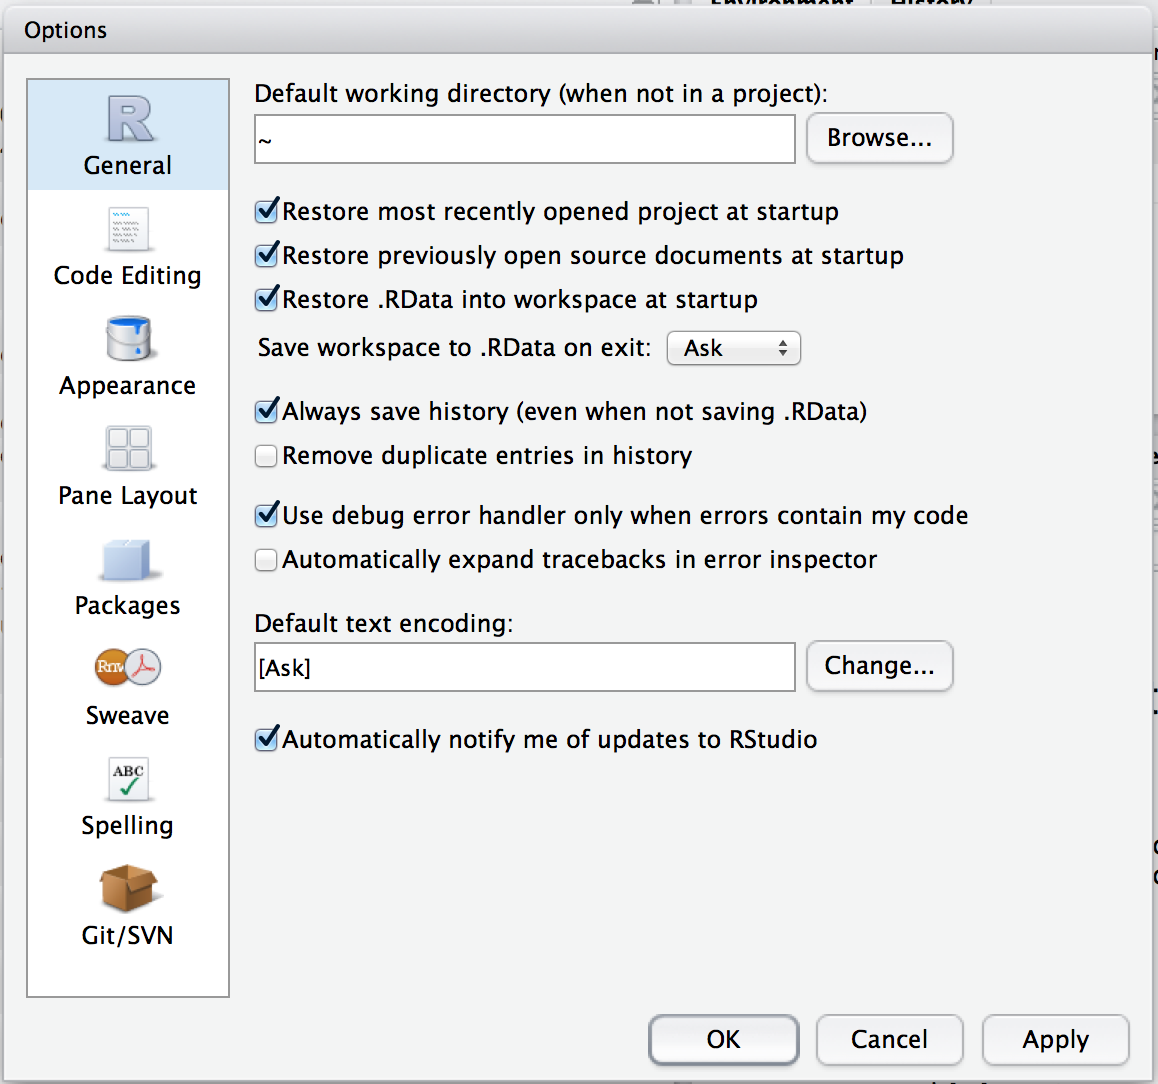
\includegraphics{/Users/dave/Documents/GitHub/stats-remix-advanced/bookdown/img/introR/Rstudio_options.png}
\caption{\label{fig:RStudiooptions}The options window in RStudio. On a Mac, you can open this window by going to the ``RStudio'' menu and selecting ``Preferences''. On a Windows machine you go to the ``Tools'' menu and select ``Global Options''}
\end{figure}

\hypertarget{summary}{%
\section{Summary}\label{summary}}

Every book that tries to introduce basic programming ideas to novices has to cover roughly the same topics, and in roughly the same order. Mine is no exception, and so in the grand tradition of doing it just the same way everyone else did it, this chapter covered the following topics:

\begin{itemize}
\tightlist
\item
  \protect\hyperlink{gettingR}{Getting started}. We downloaded and installed R and RStudio
\item
  \protect\hyperlink{arithmetic}{Basic commands}. We talked a bit about the logic of how R works and in particular how to type commands into the R console (Section @ref(\#firstcommand), and in doing so learned how to perform basic calculations using the arithmetic operators \texttt{+}, \texttt{-}, \texttt{*}, \texttt{/} and \texttt{\^{}}.
\item
  \protect\hyperlink{usingfunctions}{Introduction to functions}. We saw several different functions, three that are used to perform numeric calculations (\texttt{sqrt()}, \texttt{abs()}, \texttt{round()}, one that applies to text (\texttt{nchar()}; Section \ref{simpletext}), and one that works on any variable (\texttt{length()}; Section \ref{veclength}). In doing so, we talked a bit about how argument names work, and learned about default values for arguments. (Section \ref{functionarguments})
\item
  Introduction to variables. We learned the basic idea behind variables, and how to assign values to variables using the assignment operator \texttt{\textless{}-} (Section \ref{assign}). We also learned how to create vectors using the combine function \texttt{c()} (Section \ref{vectors}).
\item
  Data types. Learned the distinction between numeric, character and logical data; including the basics of how to enter and use each of them. (Sections \ref{assign} to \ref{logicals})
\item
  \protect\hyperlink{logicals}{Logical operations}. Learned how to use the logical operators \texttt{==}, \texttt{!=}, \texttt{\textless{}}, \texttt{\textgreater{}}, \texttt{\textless{}=}, \texttt{=\textgreater{}}, \texttt{!}, \texttt{\&} and \texttt{\textbar{}}. And learned how to use logical indexing. (Section \ref{indexing})
\end{itemize}

We still haven't arrived at anything that resembles a ``data set'', of course. Maybe the next Chapter will get us a bit closer\ldots{}

\hypertarget{mechanics}{%
\section{Additional R concepts}\label{mechanics}}

\begin{quote}
\emph{Form follows function}

-- Louis Sullivan
\end{quote}

So far, our main goal was to get started in R. As we go through the book we'll run into a lot of new R concepts, which I'll explain alongside the relevant data analysis concepts. However, there's still quite a few things that I need to talk about now, otherwise we'll run into problems when we start trying to work with data and do statistics. So that's the goal in this section: to build on the introductory content from the last section, to get you to the point that we can start using R for statistics. Broadly speaking, the section comes in two parts. The first half of the section is devoted to the ``mechanics'' of R: installing and loading packages, managing the workspace, navigating the file system, and loading and saving data. In the second half, I'll talk more about what kinds of variables exist in R, and introduce three new kinds of variables: factors, data frames and formulas. I'll finish up by talking a little bit about the help documentation in R as well as some other avenues for finding assistance. In general, I'm not trying to be comprehensive in this chapter, I'm trying to make sure that you've got the basic foundations needed to tackle the content that comes later in the book. However, a lot of the topics are revisited in more detail later, especially in Chapters \ref{datahandling} and \ref{scripting}.

\hypertarget{comments}{%
\section{Using comments}\label{comments}}

Before discussing any of the more complicated stuff, I want to introduce the \textbf{\emph{comment}} character, \texttt{\#}. It has a simple meaning: it tells R to ignore everything else you've written on this line. You won't have much need of the \texttt{\#} character immediately, but it's very useful later on when writing scripts (see Chapter \ref{scripting}). However, while you don't need to use it, I want to be able to include comments in my R extracts. For instance, if you read this:\footnote{Notice that I used \texttt{print(keeper)} rather than just typing \texttt{keeper}. Later on in the text I'll sometimes use the \texttt{print()} function to display things because I think it helps make clear what I'm doing, but in practice people rarely do this.}

\begin{Shaded}
\begin{Highlighting}[]
\NormalTok{seeker }\OtherTok{\textless{}{-}} \FloatTok{3.1415}           \CommentTok{\# create the first variable}
\NormalTok{lover }\OtherTok{\textless{}{-}} \FloatTok{2.7183}            \CommentTok{\# create the second variable}
\NormalTok{keeper }\OtherTok{\textless{}{-}}\NormalTok{ seeker }\SpecialCharTok{*}\NormalTok{ lover   }\CommentTok{\# now multiply them to create a third one}
\FunctionTok{print}\NormalTok{( keeper )            }\CommentTok{\# print out the value of \textquotesingle{}keeper\textquotesingle{}}
\end{Highlighting}
\end{Shaded}

\begin{verbatim}
## [1] 8.539539
\end{verbatim}

it's a lot easier to understand what I'm doing than if I just write this:

\begin{Shaded}
\begin{Highlighting}[]
\NormalTok{seeker }\OtherTok{\textless{}{-}} \FloatTok{3.1415}
\NormalTok{lover }\OtherTok{\textless{}{-}} \FloatTok{2.7183}
\NormalTok{keeper }\OtherTok{\textless{}{-}}\NormalTok{ seeker }\SpecialCharTok{*}\NormalTok{ lover}
\FunctionTok{print}\NormalTok{( keeper )    }
\end{Highlighting}
\end{Shaded}

\begin{verbatim}
## [1] 8.539539
\end{verbatim}

You might have already noticed that the code extracts in Chapter \ref{introR} included the \texttt{\#} character, but from now on, you'll start seeing \texttt{\#} characters appearing in the extracts, with some human-readable explanatory remarks next to them. These are still perfectly legitimate commands, since R knows that it should ignore the \texttt{\#} character and everything after it. But hopefully they'll help make things a little easier to understand.

\hypertarget{packageinstall}{%
\section{Installing and loading packages}\label{packageinstall}}

In this section I discuss R \textbf{\emph{packages}}, since almost all of the functions you might want to use in R come in packages. A package is basically just a big collection of functions, data sets and other R objects that are all grouped together under a common name. Some packages are already installed when you put R on your computer, but the vast majority of them of R packages are out there on the internet, waiting for you to download, install and use them.

When I first started writing this book, RStudio didn't really exist as a viable option for using R, and as a consequence I wrote a very lengthy section that explained how to do package management using raw R commands. It's not actually terribly hard to work with packages that way, but it's clunky and unpleasant. Fortunately, we don't have to do things that way anymore. In this section, I'll describe how to work with packages using the RStudio tools, because they're so much simpler. Along the way, you'll see that whenever you get RStudio to do something (e.g., install a package), you'll actually see the R commands that get created. I'll explain them as we go, because I think that helps you understand what's going on.

However, before we get started, there's a critical distinction that you need to understand, which is the difference between having a package \textbf{\emph{installed}} on your computer, and having a package \textbf{\emph{loaded}} in R. As of this writing, there are just over 5000 R packages freely available ``out there'' on the internet.\footnote{More precisely, there are 5000 or so packages on CRAN, the Comprehensive R Archive Network.} When you install R on your computer, you don't get all of them: only about 30 or so come bundled with the basic R installation. So right now there are about 30 packages ``installed'' on your computer, and another 5000 or so that are not installed. So that's what installed means: it means ``it's on your computer somewhere''. The critical thing to remember is that just because something is on your computer doesn't mean R can use it. In order for R to be able to \emph{use} one of your 30 or so installed packages, that package must also be ``loaded''. Generally, when you open up R, only a few of these packages (about 7 or 8) are actually loaded. Basically what it boils down to is this:

\begin{quote}
A package must be installed before it can be loaded.
\end{quote}

\begin{quote}
A package must be loaded before it can be used.
\end{quote}

This two step process might seem a little odd at first, but the designers of R had very good reasons to do it this way,\footnote{Basically, the reason is that there are 5000 packages, and probably about 4000 authors of packages, and no-one really knows what all of them do. Keeping the installation separate from the loading minimizes the chances that two packages will interact with each other in a nasty way.} and you get the hang of it pretty quickly.

\hypertarget{the-package-panel-in-rstudio}{%
\subsection{The package panel in RStudio}\label{the-package-panel-in-rstudio}}

\begin{figure}
\centering
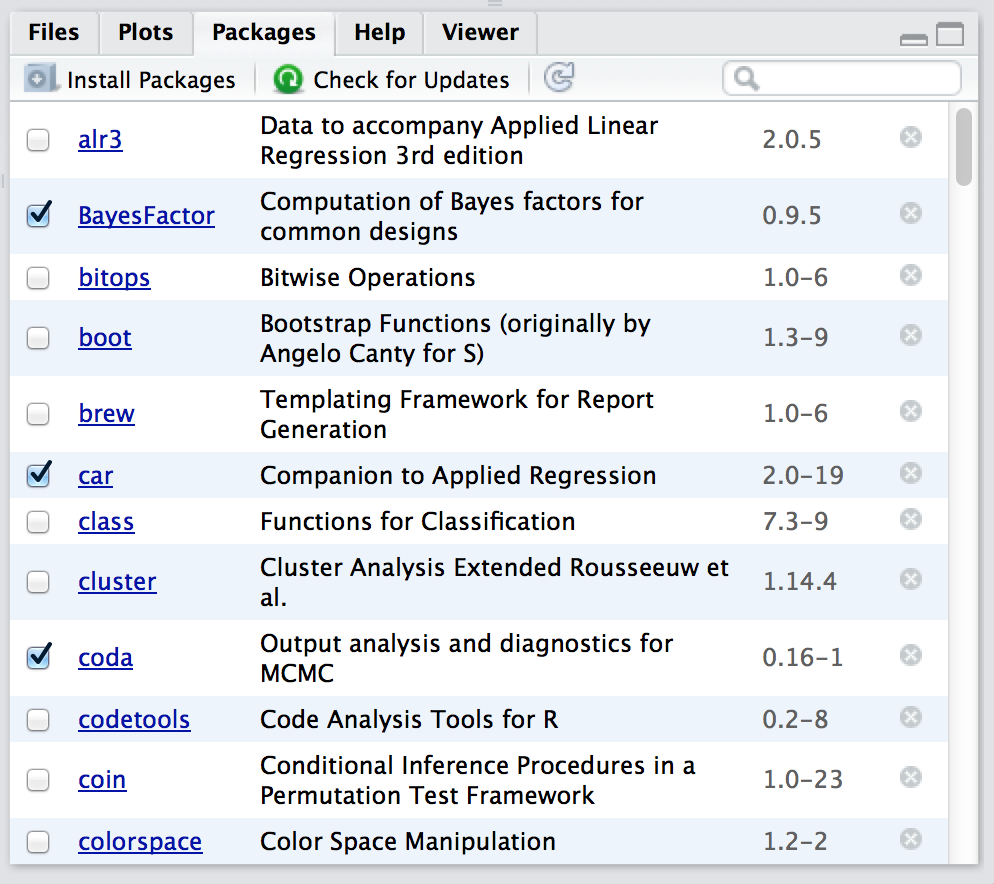
\includegraphics{/Users/dave/Documents/GitHub/stats-remix-advanced/bookdown/img/mechanics/Rstudiopackages.png}
\caption{\label{fig:packagepanel}The packages panel.}
\end{figure}

Right, lets get started. The first thing you need to do is look in the lower right hand panel in RStudio. You'll see a tab labelled ``Packages''. Click on the tab, and you'll see a list of packages that looks something like Figure \ref{fig:packagepanel}. Every row in the panel corresponds to a different package, and every column is a useful piece of information about that package.\footnote{If you're using the command line, you can get the same information by typing \texttt{library()} at the command line.} Going from left to right, here's what each column is telling you:

\begin{itemize}
\tightlist
\item
  The check box on the far left column indicates whether or not the package is loaded.
\item
  The one word of text immediately to the right of the check box is the name of the package.
\item
  The short passage of text next to the name is a brief description of the package.
\item
  The number next to the description tells you what version of the package you have installed.
\item
  The little x-mark next to the version number is a button that you can push to uninstall the package from your computer (you almost never need this).
\end{itemize}

\hypertarget{packageload}{%
\subsection{Loading a package}\label{packageload}}

That seems straightforward enough, so let's try loading and unloading packades. For this example, I'll use the \texttt{foreign} package. The \texttt{foreign} package is a collection of tools that are very handy when R needs to interact with files that are produced by other software packages (e.g., SPSS). It comes bundled with R, so it's one of the ones that you have installed already, but it won't be one of the ones loaded. Inside the \texttt{foreign} package is a function called \texttt{read.spss()}. It's a handy little function that you can use to import an SPSS data file into R, so let's pretend we want to use it. Currently, the \texttt{foreign} package isn't loaded, so if I ask R to tell me if it knows about a function called \texttt{read.spss()} it tells me that there's no such thing\ldots{}

\begin{Shaded}
\begin{Highlighting}[]
\FunctionTok{exists}\NormalTok{( }\StringTok{"read.spss"}\NormalTok{ )}
\end{Highlighting}
\end{Shaded}

\begin{verbatim}
## [1] FALSE
\end{verbatim}

Now let's load the package. In RStudio, the process is dead simple: go to the package tab, find the entry for the \texttt{foreign} package, and check the box on the left hand side. The moment that you do this, you'll see a command like this appear in the R console:

\begin{Shaded}
\begin{Highlighting}[]
\FunctionTok{library}\NormalTok{(}\StringTok{"foreign"}\NormalTok{, }\AttributeTok{lib.loc=}\StringTok{"/Library/Frameworks/R.framework/Versions/3.0/Resources/library"}\NormalTok{)}
\end{Highlighting}
\end{Shaded}

The \texttt{lib.loc} bit will look slightly different on Macs versus on Windows, because that part of the command is just RStudio telling R where to look to find the installed packages. What I've shown you above is the Mac version. On a Windows machine, you'll probably see something that looks like this:

\begin{Shaded}
\begin{Highlighting}[]
\FunctionTok{library}\NormalTok{(}\StringTok{"foreign"}\NormalTok{, }\AttributeTok{lib.loc=}\StringTok{"C:/Program Files/R/R{-}3.0.2/library"}\NormalTok{)}
\end{Highlighting}
\end{Shaded}

But actually it doesn't matter much. The \texttt{lib.loc} bit is almost always unnecessary. Unless you've taken to installing packages in idiosyncratic places (which is something that you can do if you really want) R already knows where to look. So in the vast majority of cases, the command to load the \texttt{foreign} package is just this:

\begin{Shaded}
\begin{Highlighting}[]
\FunctionTok{library}\NormalTok{(}\StringTok{"foreign"}\NormalTok{)}
\end{Highlighting}
\end{Shaded}

Throughout this book, you'll often see me typing in \texttt{library()} commands. You don't actually have to type them in yourself: you can use the RStudio package panel to do all your package loading for you. The only reason I include the \texttt{library()} commands sometimes is as a reminder to you to make sure that you have the relevant package loaded. Oh, and I suppose we should check to see if our attempt to load the package actually worked. Let's see if R now knows about the existence of the \texttt{read.spss()} function\ldots{}

\begin{Shaded}
\begin{Highlighting}[]
\FunctionTok{exists}\NormalTok{( }\StringTok{"read.spss"}\NormalTok{ )}
\end{Highlighting}
\end{Shaded}

\begin{verbatim}
## [1] TRUE
\end{verbatim}

Yep. All good.

\hypertarget{packageunload}{%
\subsection{Unloading a package}\label{packageunload}}

Sometimes, especially after a long session of working with R, you find yourself wanting to get rid of some of those packages that you've loaded. The RStudio package panel makes this exactly as easy as loading the package in the first place. Find the entry corresponding to the package you want to unload, and uncheck the box. When you do that for the \texttt{foreign} package, you'll see this command appear on screen:

\begin{Shaded}
\begin{Highlighting}[]
\FunctionTok{detach}\NormalTok{(}\StringTok{"package:foreign"}\NormalTok{, }\AttributeTok{unload=}\ConstantTok{TRUE}\NormalTok{)}
\end{Highlighting}
\end{Shaded}

And the package is unloaded. We can verify this by seeing if the \texttt{read.spss()} function still \texttt{exists()}:

\begin{Shaded}
\begin{Highlighting}[]
\FunctionTok{exists}\NormalTok{( }\StringTok{"read.spss"}\NormalTok{ )}
\end{Highlighting}
\end{Shaded}

\begin{verbatim}
## [1] FALSE
\end{verbatim}

Nope. Definitely gone.

\hypertarget{a-few-extra-comments}{%
\subsection{A few extra comments}\label{a-few-extra-comments}}

Sections \ref{packageload} and \ref{packageunload} cover the main things you need to know about loading and unloading packages. However, there's a couple of other details that I want to draw your attention to. A concrete example is the best way to illustrate. One of the other packages that you already have installed on your computer is the \texttt{Matrix} package, so let's load that one and see what happens:

\begin{Shaded}
\begin{Highlighting}[]
\FunctionTok{library}\NormalTok{( Matrix )}

\DocumentationTok{\#\# Loading required package: lattice}
\end{Highlighting}
\end{Shaded}

This is slightly more complex than the output that we got last time, but it's not too complicated. The \texttt{Matrix} package makes use of some of the tools in the \texttt{lattice} package, and R has kept track of this dependency. So when you try to load the \texttt{Matrix} package, R recognises that you're also going to need to have the \texttt{lattice} package loaded too. As a consequence, \emph{both} packages get loaded, and R prints out a helpful little note on screen to tell you that it's done so.

R is pretty aggressive about enforcing these dependencies. Suppose, for example, I try to unload the \texttt{lattice} package while the \texttt{Matrix} package is still loaded. This is easy enough to try: all I have to do is uncheck the box next to ``lattice'' in the packages panel. But if I try this, here's what happens:

\begin{Shaded}
\begin{Highlighting}[]
\FunctionTok{detach}\NormalTok{(}\StringTok{"package:lattice"}\NormalTok{, }\AttributeTok{unload=}\ConstantTok{TRUE}\NormalTok{)}

\DocumentationTok{\#\# Error: package \textasciigrave{}lattice\textquotesingle{} is required by \textasciigrave{}Matrix\textquotesingle{} so will not be detached}
\end{Highlighting}
\end{Shaded}

R refuses to do it. This can be quite useful, since it stops you from accidentally removing something that you still need. So, if I want to remove both \texttt{Matrix} and \texttt{lattice}, I need to do it in the correct order

Something else you should be aware of. Sometimes you'll attempt to load a package, and R will print out a message on screen telling you that something or other has been ``masked''. This will be confusing to you if I don't explain it now, and it actually ties very closely to the whole reason why R forces you to load packages separately from installing them. Here's an example. Two of the package that I'll refer to a lot in this book are called \texttt{car} and \texttt{psych}. The \texttt{car} package is short for ``Companion to Applied Regression'' (which is a really great book, I'll add), and it has a lot of tools that I'm quite fond of. The \texttt{car} package was written by a guy called John Fox, who has written a lot of great statistical tools for social science applications. The \texttt{psych} package was written by William Revelle, and it has a lot of functions that are very useful for psychologists in particular, especially in regards to psychometric techniques. For the most part, \texttt{car} and \texttt{psych} are quite unrelated to each other. They do different things, so not surprisingly almost all of the function names are different. But\ldots{} there's one exception to that. The \texttt{car} package and the \texttt{psych} package \emph{both} contain a function called \texttt{logit()}.\footnote{The logit function a simple mathematical function that happens not to have been included in the basic R distribution.} This creates a naming conflict. If I load both packages into R, an ambiguity is created. If the user types in \texttt{logit(100)}, should R use the \texttt{logit()} function in the \texttt{car} package, or the one in the \texttt{psych} package? The answer is: R uses whichever package you loaded most recently, and it tells you this very explicitly. Here's what happens when I load the \texttt{car} package, and then afterwards load the \texttt{psych} package:

\begin{Shaded}
\begin{Highlighting}[]
\FunctionTok{library}\NormalTok{(car)}
\end{Highlighting}
\end{Shaded}

\begin{verbatim}
## Loading required package: carData
\end{verbatim}

\begin{Shaded}
\begin{Highlighting}[]
\FunctionTok{library}\NormalTok{(psych)}
\end{Highlighting}
\end{Shaded}

\begin{verbatim}
## 
## Attaching package: 'psych'
\end{verbatim}

\begin{verbatim}
## The following object is masked from 'package:car':
## 
##     logit
\end{verbatim}

The output here is telling you that the \texttt{logit} object (i.e., function) in the \texttt{car} package is no longer accessible to you. It's been hidden (or ``masked'') from you by the one in the \texttt{psych} package.\footnote{Tip for advanced users. You can get R to use the one from the \texttt{car} package by using \texttt{car::logit()} as your command rather than \texttt{logit()}, since the \texttt{car::} part tells R explicitly which package to use. See also \texttt{:::} if you're especially keen to force R to use functions it otherwise wouldn't, but take care, since \texttt{:::} can be dangerous.}

\hypertarget{downloading-new-packages}{%
\subsection{Downloading new packages}\label{downloading-new-packages}}

One of the main selling points for R is that there are thousands of packages that have been written for it, and these are all available online. So whereabouts online are these packages to be found, and how do we download and install them? There is a big repository of packages called the ``Comprehensive R Archive Network'' (CRAN), and the easiest way of getting and installing a new package is from one of the many CRAN mirror sites. Conveniently for us, R provides a function called \texttt{install.packages()} that you can use to do this. Even \emph{more} conveniently, the RStudio team runs its own CRAN mirror and RStudio has a clean interface that lets you install packages without having to learn how to use the \texttt{install.packages()} command\footnote{It is not very difficult.}

Using the RStudio tools is, again, dead simple. In the top left hand corner of the packages panel (Figure \ref{fig:packagepanel}) you'll see a button called ``Install Packages''. If you click on that, it will bring up a window like the one shown in Figure \ref{fig:packageinstalla}.

\begin{figure}
\centering
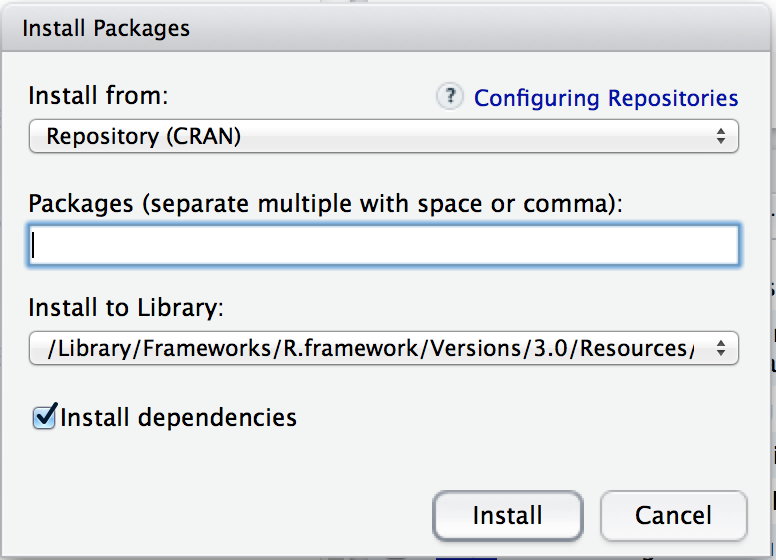
\includegraphics{/Users/dave/Documents/GitHub/stats-remix-advanced/bookdown/img/mechanics/installpackage.png}
\caption{\label{fig:packageinstalla}The package installation dialog box in RStudio}
\end{figure}

There are a few different buttons and boxes you can play with. Ignore most of them. Just go to the line that says ``Packages'' and start typing the name of the package that you want. As you type, you'll see a dropdown menu appear (Figure \ref{fig:packageinstallb}), listing names of packages that start with the letters that you've typed so far.

\begin{figure}
\centering
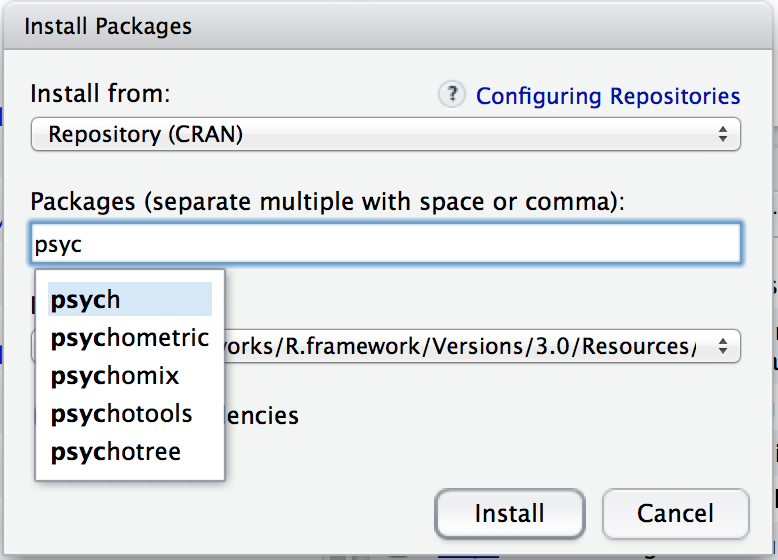
\includegraphics{/Users/dave/Documents/GitHub/stats-remix-advanced/bookdown/img/mechanics/installpackage2.png}
\caption{\label{fig:packageinstallb}When you start typing, you'll see a dropdown menu suggest a list of possible packages that you might want to install}
\end{figure}

You can select from this list, or just keep typing. Either way, once you've got the package name that you want, click on the install button at the bottom of the window. When you do, you'll see the following command appear in the R console:

\begin{Shaded}
\begin{Highlighting}[]
\FunctionTok{install.packages}\NormalTok{(}\StringTok{"psych"}\NormalTok{)}
\end{Highlighting}
\end{Shaded}

This is the R command that does all the work. R then goes off to the internet, has a conversation with CRAN, downloads some stuff, and installs it on your computer. You probably don't care about all the details of R's little adventure on the web, but the \texttt{install.packages()} function is rather chatty, so it reports a bunch of gibberish that you really aren't all that interested in:

\begin{verbatim}
trying URL 'http://cran.rstudio.com/bin/macosx/contrib/3.0/psych_1.4.1.tgz'
Content type 'application/x-gzip' length 2737873 bytes (2.6 Mb)
opened URL
==================================================
downloaded 2.6 Mb


The downloaded binary packages are in
    /var/folders/cl/thhsyrz53g73q0w1kb5z3l_80000gn/T//RtmpmQ9VT3/downloaded_packages
\end{verbatim}

Despite the long and tedious response, all thar really means is ``I've installed the psych package''. I find it best to humour the talkative little automaton. I don't actually read any of this garbage, I just politely say ``thanks'' and go back to whatever I was doing.

\hypertarget{updating-r-and-r-packages}{%
\subsection{Updating R and R packages}\label{updating-r-and-r-packages}}

Every now and then the authors of packages release updated versions. The updated versions often add new functionality, fix bugs, and so on. It's generally a good idea to update your packages periodically. There's an \texttt{update.packages()} function that you can use to do this, but it's probably easier to stick with the RStudio tool. In the packages panel, click on the ``Update Packages'' button. This will bring up a window that looks like the one shown in Figure \ref{fig:updatepackages}. In this window, each row refers to a package that needs to be updated. You can to tell R which updates you want to install by checking the boxes on the left. If you're feeling lazy and just want to update everything, click the ``Select All'' button, and then click the ``Install Updates'' button. R then prints out a \emph{lot} of garbage on the screen, individually downloading and installing all the new packages. This might take a while to complete depending on how good your internet connection is. Go make a cup of coffee. Come back, and all will be well.

\begin{figure}
\centering
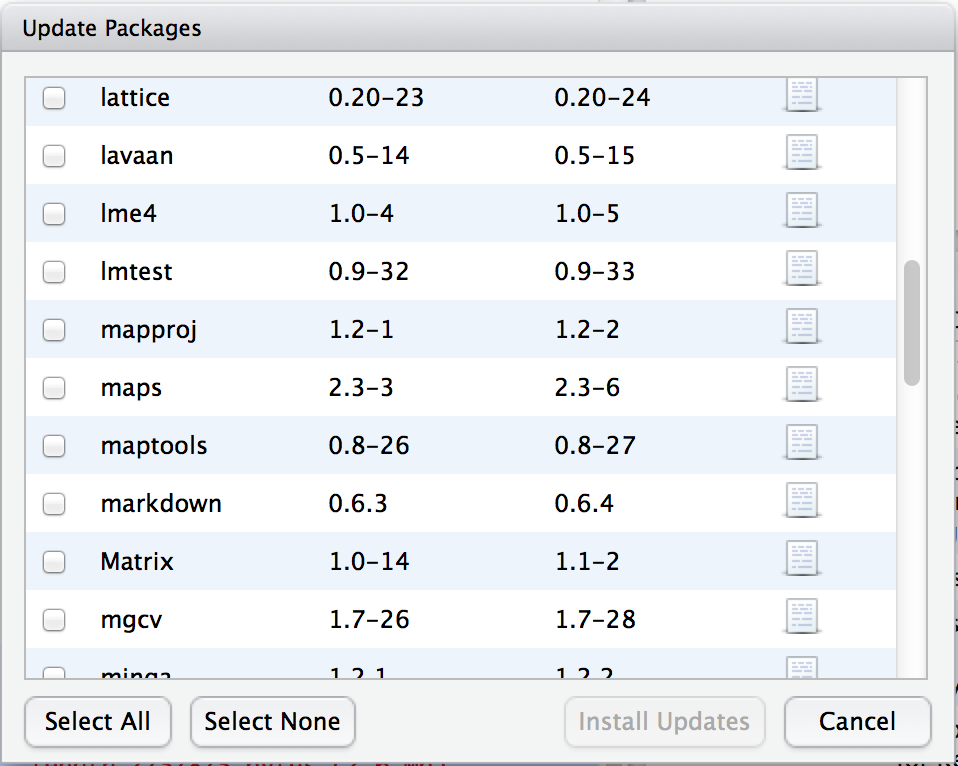
\includegraphics{/Users/dave/Documents/GitHub/stats-remix-advanced/bookdown/img/mechanics/updatepackages.png}
\caption{\label{fig:updatepackages}The RStudio dialog box for updating packages}
\end{figure}

About every six months or so, a new version of R is released. You can't update R from within RStudio (not to my knowledge, at least): to get the new version you can go to the CRAN website and download the most recent version of R, and install it in the same way you did when you originally installed R on your computer. This used to be a slightly frustrating event, because whenever you downloaded the new version of R, you would lose all the packages that you'd downloaded and installed, and would have to repeat the process of re-installing them. This was pretty annoying, and there were some neat tricks you could use to get around this. However, newer versions of R don't have this problem so I no longer bother explaining the workarounds for that issue.

\hypertarget{what-packages-does-this-book-use}{%
\subsection{What packages does this book use?}\label{what-packages-does-this-book-use}}

There are several packages that I make use of in this book. The most prominent ones are:

\begin{itemize}
\tightlist
\item
  \texttt{lsr}. This is the \emph{Learning Statistics with R} package that accompanies this book. It doesn't have a lot of interesting high-powered tools: it's just a small collection of handy little things that I think can be useful to novice users. As you get more comfortable with R this package should start to feel pretty useless to you.
\item
  \texttt{psych}. This package, written by William Revelle, includes a lot of tools that are of particular use to psychologists. In particular, there's several functions that are particularly convenient for producing analyses or summaries that are very common in psych, but less common in other disciplines.
\item
  \texttt{car}. This is the \emph{Companion to Applied Regression} package, which accompanies the excellent book of the same name by \citep{Fox2011}. It provides a lot of very powerful tools, only some of which we'll touch in this book.
\end{itemize}

Besides these three, there are a number of packages that I use in a more limited fashion: \texttt{gplots}, \texttt{sciplot}, \texttt{foreign}, \texttt{effects}, \texttt{R.matlab}, \texttt{gdata}, \texttt{lmtest}, and probably one or two others that I've missed. There are also a number of packages that I refer to but don't actually use in this book, such as \texttt{reshape}, \texttt{compute.es}, \texttt{HistData} and \texttt{multcomp} among others. Finally, there are a number of packages that provide more advanced tools that I hope to talk about in future versions of the book, such as \texttt{sem}, \texttt{ez}, \texttt{nlme} and \texttt{lme4}. In any case, whenever I'm using a function that isn't in the core packages, I'll make sure to note this in the text.

\hypertarget{workspace}{%
\section{Managing the workspace}\label{workspace}}

Let's suppose that you're reading through this book, and what you're doing is sitting down with it once a week and working through a whole chapter in each sitting. Not only that, you've been following my advice and typing in all these commands into R. So far during this chapter, you'd have typed quite a few commands, although the only ones that actually involved creating variables were the ones you typed during Section \ref{comments}. As a result, you currently have three variables; \texttt{seeker}, \texttt{lover}, and \texttt{keeper}. These three variables are the contents of your \textbf{\emph{workspace}}, also referred to as the \textbf{global environment}. The workspace is a key concept in R, so in this section we'll talk a lot about what it is and how to manage its contents.

\hypertarget{listing-the-contents-of-the-workspace}{%
\subsection{Listing the contents of the workspace}\label{listing-the-contents-of-the-workspace}}

\begin{figure}
\centering
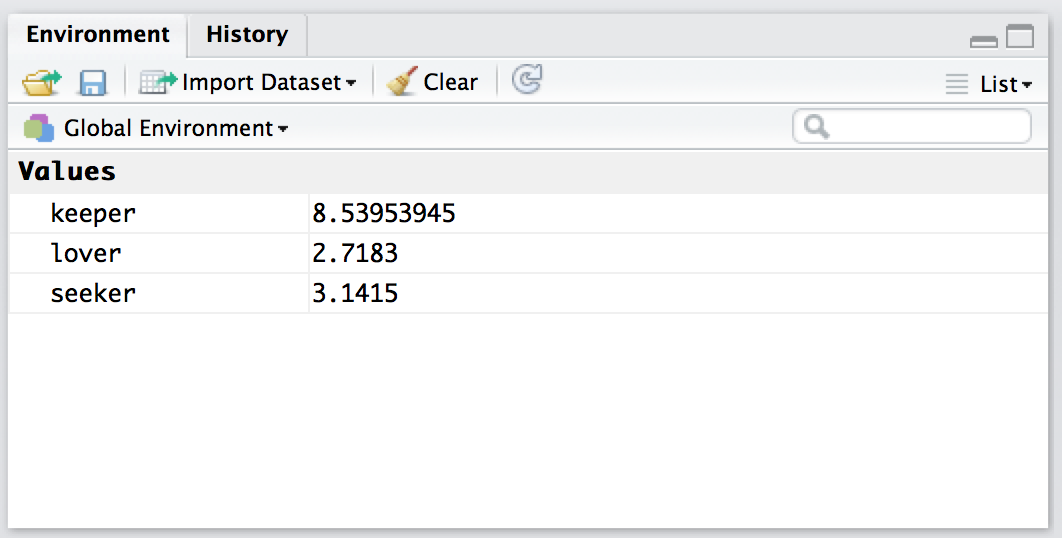
\includegraphics{/Users/dave/Documents/GitHub/stats-remix-advanced/bookdown/img/mechanics/workspacepanel.png}
\caption{\label{fig:workspace}The RStudio Environment panel shows you the contents of the workspace. The view shown above is the list view. To switch to the grid view, click on the menu item on the top right that currently reads list. Select grid from the dropdown menu, and then it will switch to a view like the one shown in the other workspace figure}
\end{figure}

\begin{figure}
\centering
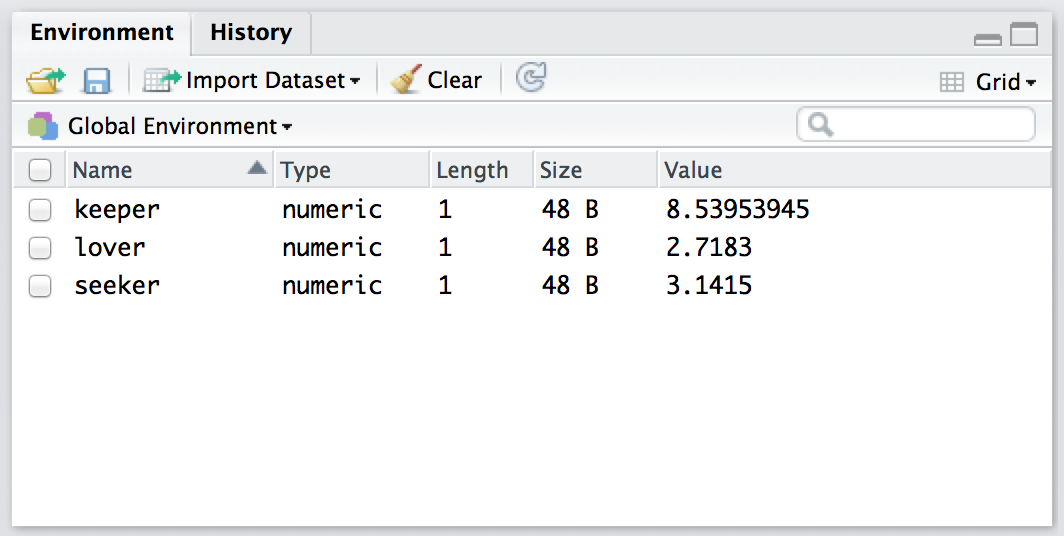
\includegraphics{/Users/dave/Documents/GitHub/stats-remix-advanced/bookdown/img/mechanics/workspacepanel2.png}
\caption{\label{fig:workspace2}The RStudio ``Environment'' panel shows you the contents of the workspace. Compare this ``grid'' view to the ``list'' earlier}
\end{figure}

The first thing that you need to know how to do is examine the contents of the workspace. If you're using RStudio, you will probably find that the easiest way to do this is to use the ``Environment'' panel in the top right hand corner. Click on that, and you'll see a list that looks very much like the one shown in Figures \ref{fig:workspace} and \ref{fig:workspace2}. If you're using the commmand line, then the \texttt{objects()} function may come in handy:

\begin{Shaded}
\begin{Highlighting}[]
\FunctionTok{objects}\NormalTok{()}
\end{Highlighting}
\end{Shaded}

\begin{verbatim}
##  [1] "any.sales.this.month" "berkeley"             "berkeley.small"      
##  [4] "coef"                 "days.per.month"       "february.sales"      
##  [7] "greeting"             "is.the.Party.correct" "keeper"              
## [10] "lover"                "months"               "profit"              
## [13] "projecthome"          "revenue"              "royalty"             
## [16] "sales"                "sales.by.month"       "seeker"              
## [19] "simpson"              "stock.levels"         "x"                   
## [22] "xlu"
\end{verbatim}

Of course, in the true R tradition, the \texttt{objects()} function has a lot of fancy capabilities that I'm glossing over in this example. Moreover there are also several other functions that you can use, including \texttt{ls()} which is pretty much identical to \texttt{objects()}, and \texttt{ls.str()} which you can use to get a fairly detailed description of all the variables in the workspace. In fact, the \texttt{lsr} package actually includes its own function that you can use for this purpose, called \texttt{who()}. The reason for using the \texttt{who()} function is pretty straightforward: in my everyday work I find that the output produced by the \texttt{objects()} command isn't \emph{quite} informative enough, because the only thing it prints out is the name of each variable; but the \texttt{ls.str()} function is \emph{too} informative, because it prints out a lot of additional information that I really don't like to look at. The \texttt{who()} function is a compromise between the two. First, now that we've got the \texttt{lsr} package installed, we need to load it:

\begin{Shaded}
\begin{Highlighting}[]
\FunctionTok{library}\NormalTok{(lsr)}
\end{Highlighting}
\end{Shaded}

and now we can use the \texttt{who()} function:

\begin{Shaded}
\begin{Highlighting}[]
\FunctionTok{who}\NormalTok{()}
\end{Highlighting}
\end{Shaded}

\begin{verbatim}
##    -- Name --             -- Class --   -- Size --
##    any.sales.this.month   logical       12        
##    berkeley               data.frame    39 x 3    
##    berkeley.small         data.frame    46 x 2    
##    coef                   numeric       2         
##    days.per.month         numeric       12        
##    february.sales         numeric       1         
##    greeting               character     1         
##    is.the.Party.correct   logical       1         
##    keeper                 numeric       1         
##    lover                  numeric       1         
##    months                 character     12        
##    profit                 numeric       12        
##    projecthome            character     1         
##    revenue                numeric       1         
##    royalty                numeric       1         
##    sales                  numeric       1         
##    sales.by.month         numeric       12        
##    seeker                 numeric       1         
##    simpson                matrix        6 x 5     
##    stock.levels           character     12        
##    x                      logical       3         
##    xlu                    numeric       1
\end{verbatim}

As you can see, the \texttt{who()} function lists all the variables and provides some basic information about what kind of variable each one is and how many elements it contains. Personally, I find this output much easier more useful than the very compact output of the \texttt{objects()} function, but less overwhelming than the extremely verbose \texttt{ls.str()} function. Throughout this book you'll see me using the \texttt{who()} function a lot. You don't have to use it yourself: in fact, I suspect you'll find it easier to look at the RStudio environment panel. But for the purposes of writing a textbook I found it handy to have a nice text based description: otherwise there would be about another 100 or so screenshots added to the book.\footnote{This would be especially annoying if you're reading an electronic copy of the book because the text displayed by the \texttt{who()} function is searchable, whereas text shown in a screen shot isn't!}

\hypertarget{removing-variables-from-the-workspace}{%
\subsection{Removing variables from the workspace}\label{removing-variables-from-the-workspace}}

Looking over that list of variables, it occurs to me that I really don't need them any more. I created them originally just to make a point, but they don't serve any useful purpose anymore, and now I want to get rid of them. I'll show you how to do this, but first I want to warn you -- there's no ``undo'' option for variable removal. Once a variable is removed, it's gone forever unless you save it to disk. I'll show you how to do \emph{that} in Section \ref{load}, but quite clearly we have no need for these variables at all, so we can safely get rid of them.

In RStudio, the easiest way to remove variables is to use the environment panel. Assuming that you're in grid view (i.e., Figure \ref{fig:workspace2}), check the boxes next to the variables that you want to delete, then click on the ``Clear'' button at the top of the panel. When you do this, RStudio will show a dialog box asking you to confirm that you really do want to delete the variables. It's always worth checking that you really do, because as RStudio is at pains to point out, you can't undo this. Once a variable is deleted, it's gone.\footnote{Mind you, all that means is that it's been removed from the workspace. If you've got the data saved to file somewhere, then that \emph{file} is perfectly safe.} In any case, if you click ``yes'', that variable will disappear from the workspace: it will no longer appear in the environment panel, and it won't show up when you use the \texttt{who()} command.

Suppose you don't access to RStudio, and you still want to remove variables. This is where the \textbf{\emph{remove}} function \texttt{rm()} comes in handy. The simplest way to use \texttt{rm()} is just to type in a (comma separated) list of all the variables you want to remove. Let's say I want to get rid of \texttt{seeker} and \texttt{lover}, but I would like to keep \texttt{keeper}. To do this, all I have to do is type:

\begin{Shaded}
\begin{Highlighting}[]
\FunctionTok{rm}\NormalTok{( seeker, lover )}
\end{Highlighting}
\end{Shaded}

There's no visible output, but if I now inspect the workspace

\begin{Shaded}
\begin{Highlighting}[]
\FunctionTok{who}\NormalTok{()}
\end{Highlighting}
\end{Shaded}

\begin{verbatim}
##    -- Name --             -- Class --   -- Size --
##    any.sales.this.month   logical       12        
##    berkeley               data.frame    39 x 3    
##    berkeley.small         data.frame    46 x 2    
##    coef                   numeric       2         
##    days.per.month         numeric       12        
##    february.sales         numeric       1         
##    greeting               character     1         
##    is.the.Party.correct   logical       1         
##    keeper                 numeric       1         
##    months                 character     12        
##    profit                 numeric       12        
##    projecthome            character     1         
##    revenue                numeric       1         
##    royalty                numeric       1         
##    sales                  numeric       1         
##    sales.by.month         numeric       12        
##    simpson                matrix        6 x 5     
##    stock.levels           character     12        
##    x                      logical       3         
##    xlu                    numeric       1
\end{verbatim}

I see that there's only the \texttt{keeper} variable left. As you can see, \texttt{rm()} can be very handy for keeping the workspace tidy.

\hypertarget{navigation}{%
\section{Navigating the file system}\label{navigation}}

In this section I talk a little about how R interacts with the file system on your computer. It's not a terribly interesting topic, but it's useful. As background to this discussion, I'll talk a bit about how file system locations work in Section \ref{filesystem}. Once upon a time \emph{everyone} who used computers could safely be assumed to understand how the file system worked, because it was impossible to successfully use a computer if you didn't! However, modern operating systems are much more ``user friendly'', and as a consequence of this they go to great lengths to hide the file system from users. So these days it's not at all uncommon for people to have used computers most of their life and not be familiar with the way that computers organise files. If you already know this stuff, skip straight to Section \ref{navigationR}. Otherwise, read on. I'll try to give a brief introduction that will be useful for those of you who have never been forced to learn how to navigate around a computer using a DOS or UNIX shell.

\hypertarget{filesystem}{%
\subsection{The file system itself}\label{filesystem}}

In this section I describe the basic idea behind file locations and file paths. Regardless of whether you're using Window, Mac OS or Linux, every file on the computer is assigned a (fairly) human readable address, and every address has the same basic structure: it describes a \emph{path} that starts from a \emph{root} location , through as series of \emph{folders} (or if you're an old-school computer user, \emph{directories}), and finally ends up at the file.

On a Windows computer the root is the physical drive\footnote{Well, the partition, technically.} on which the file is stored, and for most home computers the name of the hard drive that stores all your files is C: and therefore most file names on Windows begin with C:. After that comes the folders, and on Windows the folder names are separated by a \texttt{\textbackslash{}} symbol. So, the complete path to this book on my Windows computer might be something like this:

\begin{verbatim}
C:\Users\danRbook\LSR.pdf
\end{verbatim}

and what that \emph{means} is that the book is called LSR.pdf, and it's in a folder called \texttt{book} which itself is in a folder called dan which itself is \ldots{} well, you get the idea. On Linux, Unix and Mac OS systems, the addresses look a little different, but they're more or less identical in spirit. Instead of using the backslash, folders are separated using a forward slash, and unlike Windows, they don't treat the physical drive as being the root of the file system. So, the path to this book on my Mac might be something like this:

\begin{verbatim}
/Users/dan/Rbook/LSR.pdf
\end{verbatim}

So that's what we mean by the ``path'' to a file. The next concept to grasp is the idea of a \textbf{\emph{working directory}} and how to change it. For those of you who have used command line interfaces previously, this should be obvious already. But if not, here's what I mean. The working directory is just ``whatever folder I'm currently looking at''. Suppose that I'm currently looking for files in Explorer (if you're using Windows) or using Finder (on a Mac). The folder I currently have open is my user directory (i.e., \texttt{C:\textbackslash{}Users\textbackslash{}dan} or \texttt{/Users/dan}). That's my current working directory.

The fact that we can imagine that the program is ``in'' a particular directory means that we can talk about moving \emph{from} our current location \emph{to} a new one. What that means is that we might want to specify a new location in relation to our current location. To do so, we need to introduce two new conventions. Regardless of what operating system you're using, we use \texttt{.} to refer to the current working directory, and \texttt{..} to refer to the directory above it. This allows us to specify a path to a new location in relation to our current location, as the following examples illustrate. Let's assume that I'm using my Windows computer, and my working directory is \texttt{C:\textbackslash{}Users\textbackslash{}danRbook}). The table below shows several addresses in relation to my current one:

\begin{table}

\caption{\label{tab:unnamed-chunk-109}Basic arithmetic operations in R. These five operators are used very frequently throughout the text, so it's important to be familiar with them at the outset.}
\centering
\begin{tabular}[t]{ll}
\toprule
absolute path (i.e., from root) & relative path (i.e. from C:\textbackslash{}Users\textbackslash{}danRbook)\\
\midrule
C:\textbackslash{}\textbackslash{}Users\textbackslash{}\textbackslash{}dan & ..\\
C:\textbackslash{}\textbackslash{}Users & ..\textbackslash{}\textbackslash{}.. \textbackslash{}\textbackslash{}\\
C:\textbackslash{}\textbackslash{}Users\textbackslash{}\textbackslash{}danRbook\textbackslash{}\textbackslash{}source & .\textbackslash{}\textbackslash{}source\\
C:\textbackslash{}\textbackslash{}Users\textbackslash{}\textbackslash{}dan\textbackslash{}\textbackslash{}nerdstuff & ..\textbackslash{}\textbackslash{}nerdstuff\\
\bottomrule
\end{tabular}
\end{table}

There's one last thing I want to call attention to: the \texttt{\textasciitilde{}} directory. I normally wouldn't bother, but R makes reference to this concept sometimes. It's quite common on computers that have multiple users to define \texttt{\textasciitilde{}} to be the user's home directory. On my Mac, for instance, the home directory \texttt{\textasciitilde{}} for the ``dan'' user is \texttt{\textbackslash{}Users\textbackslash{}dan\textbackslash{}}. And so, not surprisingly, it is possible to define other directories in terms of their relationship to the home directory. For example, an alternative way to describe the location of the \texttt{LSR.pdf} file on my Mac would be

\begin{verbatim}
~Rbook\LSR.pdf
\end{verbatim}

That's about all you really need to know about file paths. And since this section already feels too long, it's time to look at how to navigate the file system in R.

\hypertarget{navigationR}{%
\subsection{Navigating the file system using the R console}\label{navigationR}}

In this section I'll talk about how to navigate this file system from within R itself. It's not particularly user friendly, and so you'll probably be happy to know that RStudio provides you with an easier method, and I will describe it in Section \ref{nav3}. So in practice, you won't \emph{really} need to use the commands that I babble on about in this section, but I do think it helps to see them in operation at least once before forgetting about them forever.

Okay, let's get started. When you want to load or save a file in R it's important to know what the working directory is. You can find out by using the \texttt{getwd()} command. For the moment, let's assume that I'm using Mac OS or Linux, since there's some subtleties to Windows. Here's what happens:

\begin{verbatim}
getwd()
## [1] "/Users/dan"
\end{verbatim}

We can change the working directory quite easily using \texttt{setwd()}. The \texttt{setwd()} function has only the one argument, \texttt{dir}, is a character string specifying a path to a directory, or a path relative to the working directory. Since I'm currently located at \texttt{/Users/dan}, the following two are equivalent:

\begin{verbatim}
setwd("/Users/dan/Rbook/data")
setwd("./Rbook/data")
\end{verbatim}

Now that we're here, we can type \texttt{list.files()} command to get a listing of all the files in that directory. Since this is the directory in which I store all of the data files that we'll use in this book, here's what we get as the result:

\begin{verbatim}
list.files()
## [1] "afl24.Rdata"             "aflsmall.Rdata"          "aflsmall2.Rdata"        
## [4] "agpp.Rdata"              "all.zip"                 "annoying.Rdata"         
## [7] "anscombesquartet.Rdata"  "awesome.Rdata"           "awesome2.Rdata"         
## [10] "booksales.csv"           "booksales.Rdata"         "booksales2.csv"         
## [13] "cakes.Rdata"             "cards.Rdata"             "chapek9.Rdata"          
## [16] "chico.Rdata"             "clinicaltrial_old.Rdata" "clinicaltrial.Rdata"    
## [19] "coffee.Rdata"            "drugs.wmc.rt.Rdata"      "dwr_all.Rdata"          
## [22] "effort.Rdata"            "happy.Rdata"             "harpo.Rdata"            
## [25] "harpo2.Rdata"            "likert.Rdata"            "nightgarden.Rdata"      
## [28] "nightgarden2.Rdata"      "parenthood.Rdata"        "parenthood2.Rdata"      
## [31] "randomness.Rdata"        "repeated.Rdata"          "rtfm.Rdata"             
## [34] "salem.Rdata"             "zeppo.Rdata"
\end{verbatim}

Not terribly exciting, I'll admit, but it's useful to know about. In any case, there's only one more thing I want to make a note of, which is that R also makes use of the home directory. You can find out what it is by using the \texttt{path.expand()} function, like this:

\begin{verbatim}
path.expand("~")
## [1] "/Users/dan"
\end{verbatim}

You can change the user directory if you want, but we're not going to make use of it very much so there's no reason to. The only reason I'm even bothering to mention it at all is that when you use RStudio to open a file, you'll see output on screen that defines the path to the file relative to the \texttt{\textasciitilde{}} directory. I'd prefer you not to be confused when you see it.\footnote{One additional thing worth calling your attention to is the \texttt{file.choose()} function. Suppose you want to load a file and you don't quite remember where it is, but would like to browse for it. Typing \texttt{file.choose()} at the command line will open a window in which you can browse to find the file; when you click on the file you want, R will print out the full path to that file. This is kind of handy.}

\hypertarget{why-do-the-windows-paths-use-the-wrong-slash}{%
\subsection{Why do the Windows paths use the wrong slash?}\label{why-do-the-windows-paths-use-the-wrong-slash}}

Let's suppose I'm on Windows. As before, I can find out what my current working directory is like this:

\begin{verbatim}
getwd()
## [1] "C:/Users/dan/
\end{verbatim}

This seems about right, but you might be wondering why R is displaying a Windows path using the wrong type of slash. The answer is slightly complicated, and has to do with the fact that R treats the \texttt{\textbackslash{}} character as ``special'' (see Section \ref{escapechars}). If you're deeply wedded to the idea of specifying a path using the Windows style slashes, then what you need to do is to type \texttt{/} whenever you mean \texttt{\textbackslash{}}. In other words, if you want to specify the working directory on a Windows computer, you need to use one of the following commands:

\begin{verbatim}
setwd( "C:/Users/dan" )
setwd( "C:\\Users\\dan" )
\end{verbatim}

It's kind of annoying to have to do it this way, but as you'll see later on in Section \ref{escapechars} it's a necessary evil. Fortunately, as we'll see in the next section, RStudio provides a much simpler way of changing directories\ldots{}

\hypertarget{nav3}{%
\subsection{Navigating the file system using the RStudio file panel}\label{nav3}}

Although I think it's important to understand how all this command line stuff works, in many (maybe even most) situations there's an easier way. For our purposes, the easiest way to navigate the file system is to make use of RStudio's built in tools. The ``file'' panel -- the lower right hand area in Figure \ref{fig:filepanel} -- is actually a pretty decent file browser. Not only can you just point and click on the names to move around the file system, you can also use it to set the working directory, and even load files.

\begin{figure}
\centering
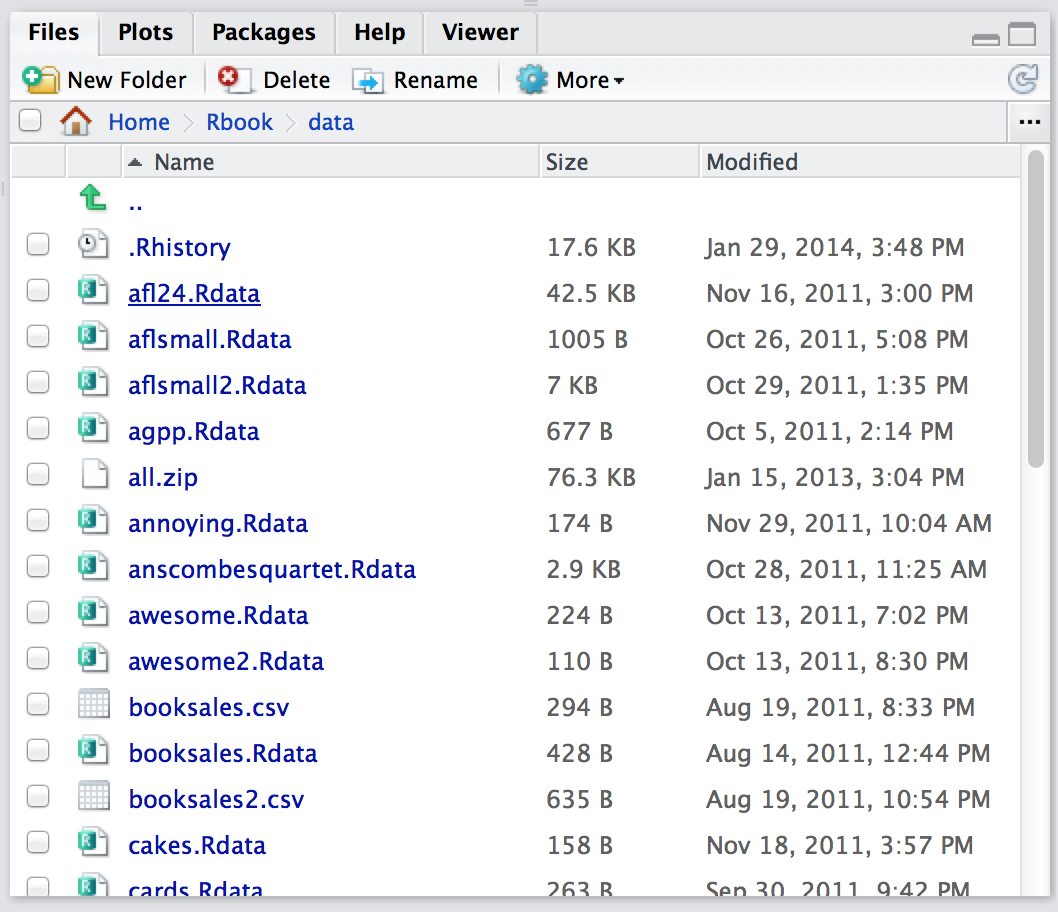
\includegraphics{/Users/dave/Documents/GitHub/stats-remix-advanced/bookdown/img/mechanics/filepanel.png}
\caption{\label{fig:filepanel}The ``file panel'' is the area shown in the lower right hand corner. It provides a very easy way to browse and navigate your computer using R. See main text for details.}
\end{figure}

Here's what you need to do to change the working directory using the file panel. Let's say I'm looking at the actual screen shown in Figure \ref{fig:filepanel}. At the top of the file panel you see some text that says ``Home \(>\) Rbook \(>\) data''. What that means is that it's \emph{displaying} the files that are stored in the

\begin{verbatim}
/Users/dan/Rbook/data
\end{verbatim}

directory on my computer. It does \emph{not} mean that this is the R working directory. If you want to change the R working directory, using the file panel, you need to click on the button that reads ``More''. This will bring up a little menu, and one of the options will be ``Set as Working Directory''. If you select that option, then R really will change the working directory. You can tell that it has done so because this command appears in the console:

\begin{verbatim}
setwd("~/Rbook/data")
\end{verbatim}

In other words, RStudio sends a command to the R console, exactly as if you'd typed it yourself. The file panel can be used to do other things too. If you want to move ``up'' to the parent folder (e.g., from \texttt{/Users/dan/Rbook/data} to \texttt{/Users/dan/Rbook} click on the ``..'' link in the file panel. To move to a subfolder, click on the name of the folder that you want to open. You can open some types of file by clicking on them. You can delete files from your computer using the ``delete'' button, rename them with the ``rename'' button, and so on.

As you can tell, the file panel is a very handy little tool for navigating the file system. But it can do more than just navigate. As we'll see later, it can be used to open files. And if you look at the buttons and menu options that it presents, you can even use it to rename, delete, copy or move files, and create new folders. However, since most of that functionality isn't critical to the basic goals of this book, I'll let you discover those on your own.

\hypertarget{load}{%
\section{Loading and saving data}\label{load}}

There are several different types of files that are likely to be relevant to us when doing data analysis. There are three in particular that are especially important from the perspective of this book:

\begin{itemize}
\tightlist
\item
  \emph{Workspace files} are those with a .Rdata file extension. This is the standard kind of file that R uses to store data and variables. They're called ``workspace files'' because you can use them to save your whole workspace.
\item
  \emph{Comma separated value (CSV) files} are those with a .csv file extension. These are just regular old text files, and they can be opened with almost any software. It's quite typical for people to store data in CSV files, precisely because they're so simple.
\item
  \emph{Script files} are those with a .R file extension. These aren't data files at all; rather, they're used to save a collection of commands that you want R to execute later. They're just text files, but we won't make use of them until Chapter \ref{scripting}.
\end{itemize}

There are also several other types of file that R makes use of,\footnote{Notably those with .rda, .Rd, .Rhistory, .rdb and .rdx extensions} but they're not really all that central to our interests. There are also several other kinds of data file that you might want to import into R. For instance, you might want to open Microsoft Excel spreadsheets (.xlsx files), or data files that have been saved in the native file formats for other statistics software, such as SPSS, SAS, Minitab, Stata or Systat. Finally, you might have to handle databases. R tries hard to play nicely with other software, so it has tools that let you open and work with any of these and many others. I'll discuss some of these other possibilities elsewhere in this book (Section \ref{importing}), but for now I want to focus primarily on the two kinds of data file that you're most likely to need: .Rdata files and .csv files.
In this section I'll talk about how to load a workspace file, how to import data from a CSV file, and how to save your workspace to a workspace file. Throughout this section I'll first describe the (sometimes awkward) R commands that do all the work, and then I'll show you the (much easier) way to do it using RStudio.

\hypertarget{loading-workspace-files-using-r}{%
\subsection{Loading workspace files using R}\label{loading-workspace-files-using-r}}

When I used the \texttt{list.files()} command to list the contents of the \texttt{/Users/dan/Rbook/data} directory (in Section \ref{navigationR}), the output referred to a file called booksales.Rdata. Let's say I want to load the data from this file into my workspace. The way I do this is with the \texttt{load()} function. There are two arguments to this function, but the only one we're interested in is

\begin{itemize}
\tightlist
\item
  \texttt{file}. This should be a character string that specifies a path to the file that needs to be loaded. You can use an absolute path or a relative path to do so.
\end{itemize}

Using the absolute file path, the command would look like this:

\begin{verbatim}
load( file = "/Users/dan/Rbook/data/booksales.Rdata" )
\end{verbatim}

but this is pretty lengthy. Given that the working directory (remember, we changed the directory at the end of Section \ref{nav3}) is \texttt{/Users/dan/Rbook/data}, I could use a relative file path, like so:

\begin{verbatim}
load( file = "../data/booksales.Rdata" )
\end{verbatim}

However, my preference is usually to change the working directory first, and \emph{then} load the file. What that would look like is this:

\begin{verbatim}
setwd( "../data" )         # move to the data directory
load( "booksales.Rdata" )  # load the data
\end{verbatim}

If I were then to type \texttt{who()} I'd see that there are several new variables in my workspace now. Throughout this book, whenever you see me loading a file, I will assume that the file is actually stored in the working directory, or that you've changed the working directory so that R is pointing at the directory that contains the file. Obviously, \emph{you} don't need type that command yourself: you can use the RStudio file panel to do the work.

\hypertarget{loading-workspace-files-using-rstudio}{%
\subsection{Loading workspace files using RStudio}\label{loading-workspace-files-using-rstudio}}

Okay, so how do we open an .Rdata file using the RStudio file panel? It's terribly simple. First, use the file panel to find the folder that contains the file you want to load. If you look at Figure \ref{fig:filepanel}, you can see that there are several .Rdata files listed. Let's say I want to load the \texttt{booksales.Rdata} file. All I have to do is click on the file name. RStudio brings up a little dialog box asking me to confirm that I do want to load this file. I click yes. The following command then turns up in the console,

\begin{verbatim}
load("~/Rbook/data/booksales.Rdata")
\end{verbatim}

and the new variables will appear in the workspace (you'll see them in the Environment panel in RStudio, or if you type \texttt{who()}). So easy it barely warrants having its own section.

\hypertarget{loadingcsv}{%
\subsection{Importing data from CSV files using loadingcsv}\label{loadingcsv}}

One quite commonly used data format is the humble ``comma separated value'' file, also called a CSV file, and usually bearing the file extension .csv. CSV files are just plain old-fashioned text files, and what they store is basically just a table of data. This is illustrated in Figure \ref{fig:booksalescsv}, which shows a file called booksales.csv that I've created. As you can see, each row corresponds to a variable, and each row represents the book sales data for one month. The first row doesn't contain actual data though: it has the names of the variables.

\begin{figure}
\centering
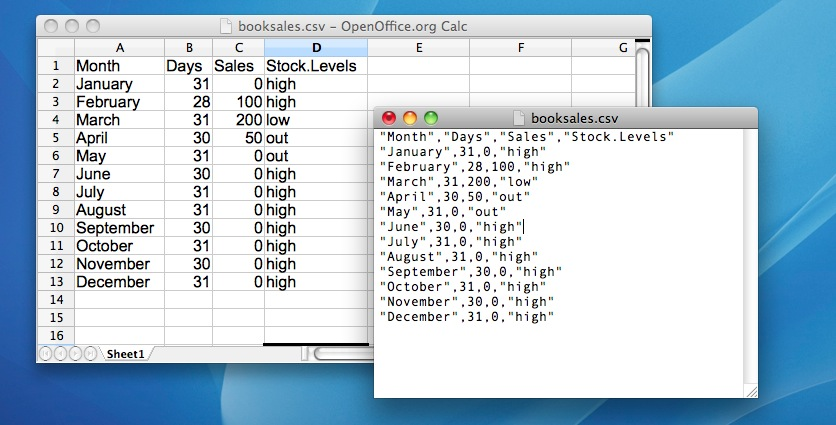
\includegraphics{/Users/dave/Documents/GitHub/stats-remix-advanced/bookdown/img/mechanics/booksalescsv.jpg}
\caption{\label{fig:booksalescsv}The booksales.csv data file. On the left, I've opened the file in using a spreadsheet program (OpenOffice), which shows that the file is basically a table. On the right, the same file is open in a standard text editor (the TextEdit program on a Mac), which shows how the file is formatted. The entries in the table are wrapped in quote marks and separated by commas.}
\end{figure}

If RStudio were not available to you, the easiest way to open this file would be to use the \texttt{read.csv()} function.\footnote{In a lot of books you'll see the \texttt{read.table()} function used for this purpose instead of \texttt{read.csv()}. They're more or less identical functions, with the same arguments and everything. They differ only in the default values.} This function is pretty flexible, and I'll talk a lot more about it's capabilities in Section \ref{importing} for more details, but for now there's only two arguments to the function that I'll mention:

\begin{itemize}
\tightlist
\item
  \texttt{file}. This should be a character string that specifies a path to the file that needs to be loaded. You can use an absolute path or a relative path to do so.
\item
  \texttt{header}. This is a logical value indicating whether or not the first row of the file contains variable names. The default value is \texttt{TRUE}.
\end{itemize}

Therefore, to import the CSV file, the command I need is:

\begin{Shaded}
\begin{Highlighting}[]
\NormalTok{books }\OtherTok{\textless{}{-}} \FunctionTok{read.csv}\NormalTok{( }\AttributeTok{file =} \StringTok{"booksales.csv"}\NormalTok{ )}
\end{Highlighting}
\end{Shaded}

There are two very important points to notice here. Firstly, notice that I \emph{didn't} try to use the \texttt{load()} function, because that function is only meant to be used for .Rdata files. If you try to use \texttt{load()} on other types of data, you get an error. Secondly, notice that when I imported the CSV file I assigned the result to a variable, which I imaginatively called \texttt{books}.\footnote{Note that I didn't to this in my earlier example when loading the .Rdata} file. There's a reason for this. The idea behind an \texttt{.Rdata} file is that it stores a whole workspace. So, if you had the ability to look inside the file yourself you'd see that the data file keeps track of all the variables and their names. So when you \texttt{load()} the file, R restores all those original names. CSV files are treated differently: as far as R is concerned, the CSV only stores \emph{one} variable, but that variable is big table. So when you import that table into the workspace, R expects \emph{you} to give it a name.{]} Let's have a look at what we've got:

\begin{Shaded}
\begin{Highlighting}[]
\FunctionTok{print}\NormalTok{( books )}
\end{Highlighting}
\end{Shaded}

\begin{verbatim}
##        Month Days Sales Stock.Levels
## 1    January   31     0         high
## 2   February   28   100         high
## 3      March   31   200          low
## 4      April   30    50          out
## 5        May   31     0          out
## 6       June   30     0         high
## 7       July   31     0         high
## 8     August   31     0         high
## 9  September   30     0         high
## 10   October   31     0         high
## 11  November   30     0         high
## 12  December   31     0         high
\end{verbatim}

Clearly, it's worked, but the format of this output is a bit unfamiliar. We haven't seen anything like this before. What you're looking at is a \emph{data frame}, which is a very important kind of variable in R, and one I'll discuss in Section \ref{dataframes}. For now, let's just be happy that we imported the data and that it looks about right.

\hypertarget{importing-data-from-csv-files-using-rstudio}{%
\subsection{Importing data from CSV files using RStudio}\label{importing-data-from-csv-files-using-rstudio}}

Yet again, it's easier in RStudio. In the environment panel in RStudio you should see a button called ``Import Dataset''. Click on that, and it will give you a couple of options: select the ``From Text File\ldots{}'' option, and it will open up a very familiar dialog box asking you to select a file: if you're on a Mac, it'll look like the usual Finder window that you use to choose a file; on Windows it looks like an Explorer window. An example of what it looks like on a Mac is shown in Figure \ref{fig:fileopen}. I'm assuming that you're familiar with your own computer, so you should have no problem finding the CSV file that you want to import! Find the one you want, then click on the ``Open'' button. When you do this, you'll see a window that looks like the one in Figure \ref{fig:import}.

\begin{figure}
\centering
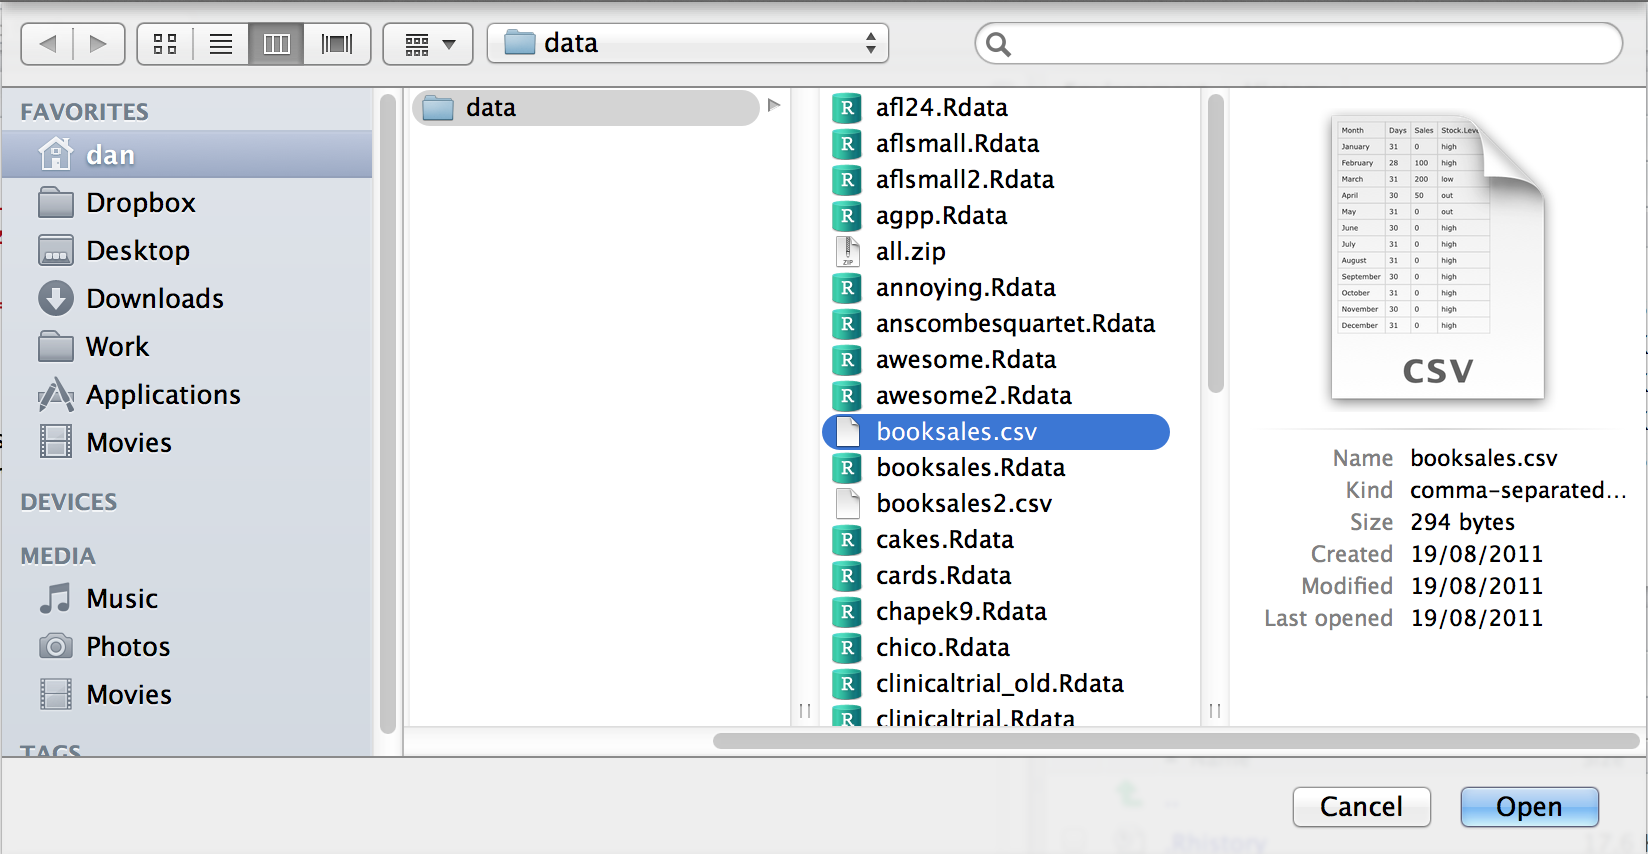
\includegraphics{/Users/dave/Documents/GitHub/stats-remix-advanced/bookdown/img/mechanics/openscreen.png}
\caption{\label{fig:fileopen}A dialog box on a Mac asking you to select the CSV file R should try to import. Mac users will recognise this immediately: it's the usual way in which a Mac asks you to find a file. Windows users won't see this: they'll see the usual explorer window that Windows always gives you when it wants you to select a file.}
\end{figure}

The import data set window is relatively straightforward to understand.

\begin{figure}
\centering
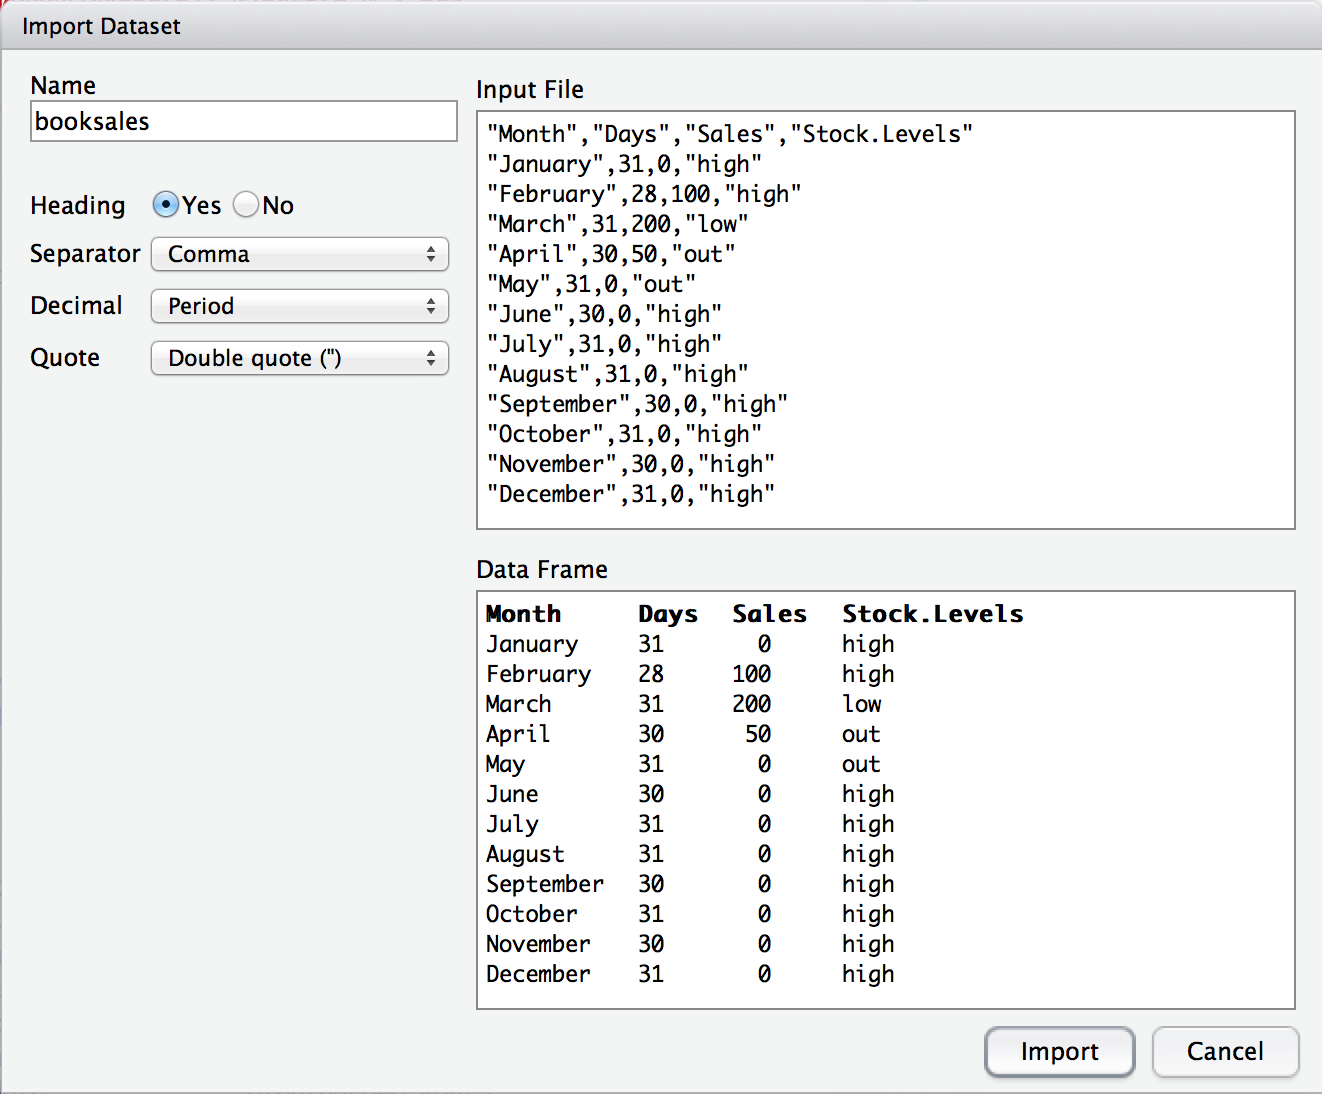
\includegraphics{/Users/dave/Documents/GitHub/stats-remix-advanced/bookdown/img/mechanics/import.png}
\caption{\label{fig:import}The RStudio window for importing a CSV file into R}
\end{figure}

In the top left corner, you need to type the name of the variable you R to create. By default, that will be the same as the file name: our file is called \texttt{booksales.csv}, so RStudio suggests the name \texttt{booksales}. If you're happy with that, leave it alone. If not, type something else. Immediately below this are a few things that you can tweak to make sure that the data gets imported correctly:

\begin{itemize}
\tightlist
\item
  Heading. Does the first row of the file contain raw data, or does it contain headings for each variable? The \texttt{booksales.csv} file has a header at the top, so I selected ``yes''.
\item
  Separator. What character is used to separate different entries? In most CSV files this will be a comma (it is ``comma separated'' after all). But you can change this if your file is different.
\item
  Decimal. What character is used to specify the decimal point? In English speaking countries, this is almost always a period (i.e., \texttt{.}). That's not universally true: many European countries use a comma. So you can change that if you need to.
\item
  Quote. What character is used to denote a block of text? That's usually going to be a double quote mark. It is for the \texttt{booksales.csv} file, so that's what I selected.
\end{itemize}

The nice thing about the RStudio window is that it shows you the raw data file at the top of the window, and it shows you a preview of the data at the bottom. If the data at the bottom doesn't look right, try changing some of the settings on the left hand side. Once you're happy, click ``Import''. When you do, two commands appear in the R console:

\begin{verbatim}
booksales <- read.csv("~/Rbook/data/booksales.csv")
View(booksales)
\end{verbatim}

The first of these commands is the one that loads the data. The second one will display a pretty table showing the data in RStudio.

\hypertarget{saving-a-workspace-file-using-save}{%
\subsection{\texorpdfstring{Saving a workspace file using \texttt{save}}{Saving a workspace file using save}}\label{saving-a-workspace-file-using-save}}

Not surprisingly, saving data is very similar to loading data. Although RStudio provides a simple way to save files (see below), it's worth understanding the actual commands involved. There are two commands you can use to do this, \texttt{save()} and \texttt{save.image()}. If you're happy to save \emph{all} of the variables in your workspace into the data file, then you should use \texttt{save.image()}. And if you're happy for R to save the file into the current working directory, all you have to do is this:

\begin{Shaded}
\begin{Highlighting}[]
\FunctionTok{save.image}\NormalTok{( }\AttributeTok{file =} \StringTok{"myfile.Rdata"}\NormalTok{ )}
\end{Highlighting}
\end{Shaded}

Since \texttt{file} is the first argument, you can shorten this to \texttt{save.image("myfile.Rdata")}; and if you want to save to a different directory, then (as always) you need to be more explicit about specifying the path to the file, just as we discussed in Section \ref{navigation}. Suppose, however, I have several variables in my workspace, and I only want to save some of them. For instance, I might have this as my workspace:

\begin{Shaded}
\begin{Highlighting}[]
\FunctionTok{who}\NormalTok{()}
\DocumentationTok{\#\#   {-}{-} Name {-}{-}   {-}{-} Class {-}{-}   {-}{-} Size {-}{-}}
\DocumentationTok{\#\#   data         data.frame    3 x 2     }
\DocumentationTok{\#\#   handy        character     1         }
\DocumentationTok{\#\#   junk         numeric       1        }
\end{Highlighting}
\end{Shaded}

I want to save \texttt{data} and \texttt{handy}, but not \texttt{junk}. But I don't want to delete \texttt{junk} right now, because I want to use it for something else later on. This is where the \texttt{save()} function is useful, since it lets me indicate exactly which variables I want to save. Here is one way I can use the \texttt{save} function to solve my problem:

\begin{Shaded}
\begin{Highlighting}[]
\FunctionTok{save}\NormalTok{(data, handy, }\AttributeTok{file =} \StringTok{"myfile.Rdata"}\NormalTok{)}
\end{Highlighting}
\end{Shaded}

Importantly, you \emph{must} specify the name of the \texttt{file} argument. The reason is that if you don't do so, R will think that \texttt{"myfile.Rdata"} is actually a \emph{variable} that you want to save, and you'll get an error message. Finally, I should mention a second way to specify which variables the \texttt{save()} function should save, which is to use the \texttt{list} argument. You do so like this:

\begin{Shaded}
\begin{Highlighting}[]
\NormalTok{save.me }\OtherTok{\textless{}{-}} \FunctionTok{c}\NormalTok{(}\StringTok{"data"}\NormalTok{, }\StringTok{"handy"}\NormalTok{)   }\CommentTok{\# the variables to be saved}
\FunctionTok{save}\NormalTok{( }\AttributeTok{file =} \StringTok{"booksales2.Rdata"}\NormalTok{, }\AttributeTok{list =}\NormalTok{ save.me )   }\CommentTok{\# the command to save them}
\end{Highlighting}
\end{Shaded}

\hypertarget{save1}{%
\subsection{Saving a workspace file using RStudio}\label{save1}}

RStudio allows you to save the workspace pretty easily. In the environment panel (Figures \ref{fig:workspace} and \ref{fig:workspace2}) you can see the ``save'' button. There's no text, but it's the same icon that gets used on every computer everywhere: it's the one that looks like a floppy disk. You know, those things that haven't been used in about 20 years. Alternatively, go to the ``Session'' menu and click on the ``Save Workspace As\ldots{}'' option.\footnote{A word of warning: what you \emph{don't} want to do is use the ``File'' menu. If you look in the ``File'' menu you will see ``Save'' and ``Save As\ldots{}'' options, but they don't save the workspace. Those options are used for dealing with \emph{scripts}, and so they'll produce \texttt{.R} files. We won't get to those until Chapter \ref{scripting}.} This will bring up the standard ``save'' dialog box for your operating system (e.g., on a Mac it'll look a little bit like the loading dialog box in Figure \ref{fig:fileopen}). Type in the name of the file that you want to save it to, and all the variables in your workspace will be saved to disk. You'll see an R command like this one

\begin{Shaded}
\begin{Highlighting}[]
\FunctionTok{save.image}\NormalTok{(}\StringTok{"\textasciitilde{}/Desktop/Untitled.RData"}\NormalTok{)}
\end{Highlighting}
\end{Shaded}

Pretty straightforward, really.

\hypertarget{other-things-you-might-want-to-save}{%
\subsection{Other things you might want to save}\label{other-things-you-might-want-to-save}}

Until now, we've talked mostly about loading and saving \emph{data}. Other things you might want to save include:

\begin{itemize}
\item
  \emph{The output}. Sometimes you might also want to keep a copy of all your interactions with R, including everything that you typed in and everything that R did in response. There are some functions that you can use to get R to write its output to a file rather than to print onscreen (e.g., \texttt{sink()}), but to be honest, if you do want to save the R output, the easiest thing to do is to use the mouse to select the relevant text in the R console, go to the ``Edit'' menu in RStudio and select ``Copy''. The output has now been copied to the clipboard. Now open up your favourite text editor or word processing software, and paste it. And you're done. However, this will only save the contents of the console, not the plots you've drawn (assuming you've drawn some). We'll talk about saving images later on.
\item
  \emph{A script}. While it is possible -- and sometimes handy -- to save the R output as a method for keeping a copy of your statistical analyses, another option that people use a lot (especially when you move beyond simple ``toy'' analyses) is to write \emph{scripts}. A script is a text file in which you write out all the commands that you want R to run. You can write your script using whatever software you like. In real world data analysis writing scripts is a key skill -- and as you become familiar with R you'll probably find that most of what you do involves scripting rather than typing commands at the R prompt. However, you won't need to do much scripting initially, so we'll leave that until Chapter \ref{scripting}.
\end{itemize}

\hypertarget{useful}{%
\section{Useful things to know about variables}\label{useful}}

In Chapter \ref{introR} I talked a lot about variables, how they're assigned and some of the things you can do with them, but there's a lot of additional complexities. That's not a surprise of course. However, some of those issues are worth drawing your attention to now. So that's the goal of this section; to cover a few extra topics. As a consequence, this section is basically a bunch of things that I want to briefly mention, but don't really fit in anywhere else. In short, I'll talk about several different issues in this section, which are only loosely connected to one another.

\hypertarget{specials}{%
\subsection{Special values}\label{specials}}

The first thing I want to mention are some of the ``special'' values that you might see R produce. Most likely you'll see them in situations where you were expecting a number, but there are quite a few other ways you can encounter them. These values are \texttt{Inf}, \texttt{NaN}, \texttt{NA} and \texttt{NULL}. These values can crop up in various different places, and so it's important to understand what they mean.

\begin{itemize}
\tightlist
\item
  \emph{Infinity} (\texttt{Inf}). The easiest of the special values to explain is \texttt{Inf}, since it corresponds to a value that is infinitely large. You can also have \texttt{-Inf}. The easiest way to get \texttt{Inf} is to divide a positive number by 0:
\end{itemize}

\begin{Shaded}
\begin{Highlighting}[]
\DecValTok{1} \SpecialCharTok{/} \DecValTok{0}
\end{Highlighting}
\end{Shaded}

\begin{verbatim}
## [1] Inf
\end{verbatim}

In most real world data analysis situations, if you're ending up with infinite numbers in your data, then something has gone awry. Hopefully you'll never have to see them.

\begin{itemize}
\tightlist
\item
  \emph{Not a Number} (\texttt{NaN}). The special value of \texttt{NaN} is short for ``not a number'', and it's basically a reserved keyword that means ``there isn't a mathematically defined number for this''. If you can remember your high school maths, remember that it is conventional to say that \(0/0\) doesn't have a proper answer: mathematicians would say that \(0/0\) is \emph{undefined}. R says that it's not a number:
\end{itemize}

\begin{Shaded}
\begin{Highlighting}[]
 \DecValTok{0} \SpecialCharTok{/} \DecValTok{0}
\end{Highlighting}
\end{Shaded}

\begin{verbatim}
## [1] NaN
\end{verbatim}

Nevertheless, it's still treated as a ``numeric'' value. To oversimplify, \texttt{NaN} corresponds to cases where you asked a proper numerical question that genuinely has \emph{no meaningful answer}.

\begin{itemize}
\item
  \emph{Not available} (\texttt{NA}).
  \texttt{NA} indicates that the value that is ``supposed'' to be stored here is missing. To understand what this means, it helps to recognise that the \texttt{NA} value is something that you're most likely to see when analysing data from real world experiments. Sometimes you get equipment failures, or you lose some of the data, or whatever. The point is that some of the information that you were ``expecting'' to get from your study is just plain missing. Note the difference between \texttt{NA} and \texttt{NaN}. For \texttt{NaN}, we really do know what's supposed to be stored; it's just that it happens to correspond to something like \(0/0\) that doesn't make any sense at all. In contrast, \texttt{NA} indicates that we actually don't know what was supposed to be there. The information is \emph{missing}.
\item
  \emph{No value} (\texttt{NULL}).
  The \texttt{NULL} value takes this ``absence'' concept even further. It basically asserts that the variable genuinely has no value whatsoever. This is quite different to both \texttt{NaN} and \texttt{NA}. For \texttt{NaN} we actually know what the value is, because it's something insane like \(0/0\). For \texttt{NA}, we believe that there is supposed to be a value ``out there'', but a dog ate our homework and so we don't quite know what it is. But for \texttt{NULL} we strongly believe that there is \emph{no value at all}.
\end{itemize}

\hypertarget{names}{%
\subsection{Assigning names to vector elements}\label{names}}

One thing that is sometimes a little unsatisfying about the way that R prints out a vector is that the elements come out unlabelled. Here's what I mean. Suppose I've got data reporting the quarterly profits for some company. If I just create a no-frills vector, I have to rely on memory to know which element corresponds to which event. That is:

\begin{Shaded}
\begin{Highlighting}[]
\NormalTok{profit }\OtherTok{\textless{}{-}} \FunctionTok{c}\NormalTok{( }\FloatTok{3.1}\NormalTok{, }\FloatTok{0.1}\NormalTok{, }\SpecialCharTok{{-}}\FloatTok{1.4}\NormalTok{, }\FloatTok{1.1}\NormalTok{ )}
\NormalTok{profit}
\end{Highlighting}
\end{Shaded}

\begin{verbatim}
## [1]  3.1  0.1 -1.4  1.1
\end{verbatim}

You can probably guess that the first element corresponds to the first quarter, the second element to the second quarter, and so on, but that's only because I've told you the back story and because this happens to be a very simple example. In general, it can be quite difficult. This is where it can be helpful to assign \texttt{names} to each of the elements. Here's how you do it:

\begin{Shaded}
\begin{Highlighting}[]
\FunctionTok{names}\NormalTok{(profit) }\OtherTok{\textless{}{-}} \FunctionTok{c}\NormalTok{(}\StringTok{"Q1"}\NormalTok{,}\StringTok{"Q2"}\NormalTok{,}\StringTok{"Q3"}\NormalTok{,}\StringTok{"Q4"}\NormalTok{)}
\NormalTok{profit}
\end{Highlighting}
\end{Shaded}

\begin{verbatim}
##   Q1   Q2   Q3   Q4 
##  3.1  0.1 -1.4  1.1
\end{verbatim}

This is a slightly odd looking command, admittedly, but it's not too difficult to follow. All we're doing is assigning a vector of labels (character strings) to \texttt{names(profit)}. You can always delete the names again by using the command \texttt{names(profit)\ \textless{}-\ NULL}. It's also worth noting that you don't have to do this as a two stage process. You can get the same result with this command:

\begin{Shaded}
\begin{Highlighting}[]
\NormalTok{profit }\OtherTok{\textless{}{-}} \FunctionTok{c}\NormalTok{( }\StringTok{"Q1"} \OtherTok{=} \FloatTok{3.1}\NormalTok{, }\StringTok{"Q2"} \OtherTok{=} \FloatTok{0.1}\NormalTok{, }\StringTok{"Q3"} \OtherTok{=} \SpecialCharTok{{-}}\FloatTok{1.4}\NormalTok{, }\StringTok{"Q4"} \OtherTok{=} \FloatTok{1.1}\NormalTok{ )}
\NormalTok{profit}
\end{Highlighting}
\end{Shaded}

\begin{verbatim}
##   Q1   Q2   Q3   Q4 
##  3.1  0.1 -1.4  1.1
\end{verbatim}

The important things to notice are that (a) this does make things much easier to read, but (b) the names at the top aren't the ``real'' data. The \emph{value} of \texttt{profit{[}1{]}} is still \texttt{3.1}; all I've done is added a \emph{name} to \texttt{profit{[}1{]}} as well. Nevertheless, names aren't purely cosmetic, since R allows you to pull out particular elements of the vector by referring to their names:

\begin{Shaded}
\begin{Highlighting}[]
\NormalTok{profit[}\StringTok{"Q1"}\NormalTok{]}
\end{Highlighting}
\end{Shaded}

\begin{verbatim}
##  Q1 
## 3.1
\end{verbatim}

And if I ever need to pull out the names themselves, then I just type \texttt{names(profit)}.

\hypertarget{variable-classes}{%
\subsection{Variable classes}\label{variable-classes}}

As we've seen, R allows you to store different kinds of data. In particular, the variables we've defined so far have either been character data (text), numeric data, or logical data.\footnote{Or functions. But let's ignore functions for the moment.} It's important that we remember what kind of information each variable stores (and even more important that R remembers) since different kinds of variables allow you to do different things to them. For instance, if your variables have numerical information in them, then it's okay to multiply them together:

\begin{Shaded}
\begin{Highlighting}[]
\NormalTok{x }\OtherTok{\textless{}{-}} \DecValTok{5}   \CommentTok{\# x is numeric}
\NormalTok{y }\OtherTok{\textless{}{-}} \DecValTok{4}   \CommentTok{\# y is numeric}
\NormalTok{x }\SpecialCharTok{*}\NormalTok{ y    }
\end{Highlighting}
\end{Shaded}

\begin{verbatim}
## [1] 20
\end{verbatim}

But if they contain character data, multiplication makes no sense whatsoever, and R will complain if you try to do it:

\begin{Shaded}
\begin{Highlighting}[]
\NormalTok{x }\OtherTok{\textless{}{-}} \StringTok{"apples"}   \CommentTok{\# x is character}
\NormalTok{y }\OtherTok{\textless{}{-}} \StringTok{"oranges"}  \CommentTok{\# y is character}
\NormalTok{x }\SpecialCharTok{*}\NormalTok{ y           }
\end{Highlighting}
\end{Shaded}

\begin{verbatim}
## Error in x * y: non-numeric argument to binary operator
\end{verbatim}

Even R is smart enough to know you can't multiply \texttt{"apples"} by \texttt{"oranges"}. It knows this because the quote marks are indicators that the variable is supposed to be treated as text, not as a number.

This is quite useful, but notice that it means that R makes a big distinction between \texttt{5} and \texttt{"5"}. Without quote marks, R treats \texttt{5} as the number five, and will allow you to do calculations with it. With the quote marks, R treats \texttt{"5"} as the textual character five, and doesn't recognise it as a number any more than it recognises \texttt{"p"} or \texttt{"five"} as numbers. As a consequence, there's a big difference between typing \texttt{x\ \textless{}-\ 5} and typing \texttt{x\ \textless{}-\ "5"}. In the former, we're storing the number \texttt{5}; in the latter, we're storing the character \texttt{"5"}. Thus, if we try to do multiplication with the character versions, R gets stroppy:

\begin{Shaded}
\begin{Highlighting}[]
\NormalTok{x }\OtherTok{\textless{}{-}} \StringTok{"5"}   \CommentTok{\# x is character}
\NormalTok{y }\OtherTok{\textless{}{-}} \StringTok{"4"}   \CommentTok{\# y is character}
\NormalTok{x }\SpecialCharTok{*}\NormalTok{ y     }
\end{Highlighting}
\end{Shaded}

\begin{verbatim}
## Error in x * y: non-numeric argument to binary operator
\end{verbatim}

Okay, let's suppose that I've forgotten what kind of data I stored in the variable \texttt{x} (which happens depressingly often). R provides a function that will let us find out. Or, more precisely, it provides \emph{three} functions: \texttt{class()}, \texttt{mode()} and \texttt{typeof()}. Why the heck does it provide three functions, you might be wondering? Basically, because R actually keeps track of three different kinds of information about a variable:

\begin{enumerate}
\def\labelenumi{\arabic{enumi}.}
\tightlist
\item
  The \textbf{\emph{class}} of a variable is a ``high level'' classification, and it captures psychologically (or statistically) meaningful distinctions. For instance \texttt{"2011-09-12"} and \texttt{"my\ birthday"} are both text strings, but there's an important difference between the two: one of them is a date. So it would be nice if we could get R to recognise that \texttt{"2011-09-12"} is a date, and allow us to do things like add or subtract from it. The class of a variable is what R uses to keep track of things like that. Because the class of a variable is critical for determining what R can or can't do with it, the \texttt{class()} function is very handy.
\item
  The \textbf{\emph{mode}} of a variable refers to the format of the information that the variable stores. It tells you whether R has stored text data or numeric data, for instance, which is kind of useful, but it only makes these ``simple'' distinctions. It can be useful to know about, but it's not the main thing we care about. So I'm not going to use the \texttt{mode()} function very much.\footnote{Actually, I don't think I \emph{ever} use this in practice. I don't know why I bother to talk about it in the book anymore.}
\item
  The \textbf{\emph{type}} of a variable is a very low level classification. We won't use it in this book, but (for those of you that care about these details) this is where you can see the distinction between integer data, double precision numeric, etc. Almost none of you actually will care about this, so I'm not even going to bother demonstrating the \texttt{typeof()} function.
\end{enumerate}

For purposes, it's the \texttt{class()} of the variable that we care most about. Later on, I'll talk a bit about how you can convince R to ``coerce'' a variable to change from one class to another (Section \ref{coercion}). That's a useful skill for real world data analysis, but it's not something that we need right now. In the meantime, the following examples illustrate the use of the \texttt{class()} function:

\begin{Shaded}
\begin{Highlighting}[]
\NormalTok{x }\OtherTok{\textless{}{-}} \StringTok{"hello world"}     \CommentTok{\# x is text}
\FunctionTok{class}\NormalTok{(x)}
\end{Highlighting}
\end{Shaded}

\begin{verbatim}
## [1] "character"
\end{verbatim}

\begin{Shaded}
\begin{Highlighting}[]
\NormalTok{x }\OtherTok{\textless{}{-}} \ConstantTok{TRUE}     \CommentTok{\# x is logical }
\FunctionTok{class}\NormalTok{(x)}
\end{Highlighting}
\end{Shaded}

\begin{verbatim}
## [1] "logical"
\end{verbatim}

\begin{Shaded}
\begin{Highlighting}[]
\NormalTok{x }\OtherTok{\textless{}{-}} \DecValTok{100}     \CommentTok{\# x is a number}
\FunctionTok{class}\NormalTok{(x)}
\end{Highlighting}
\end{Shaded}

\begin{verbatim}
## [1] "numeric"
\end{verbatim}

Exciting, no?

\hypertarget{factors}{%
\section{Factors}\label{factors}}

Okay, it's time to start introducing some of the data types that are somewhat more specific to statistics. If you remember back to Chapter \ref{studydesign}, when we assign numbers to possible outcomes, these numbers can mean quite different things depending on what kind of variable we are attempting to measure. In particular, we commonly make the distinction between \emph{nominal}, \emph{ordinal}, \emph{interval} and \emph{ratio} scale data. How do we capture this distinction in R? Currently, we only seem to have a single numeric data type. That's probably not going to be enough, is it?

A little thought suggests that the numeric variable class in R is perfectly suited for capturing ratio scale data. For instance, if I were to measure response time (RT) for five different events, I could store the data in R like this:

\begin{Shaded}
\begin{Highlighting}[]
\NormalTok{RT }\OtherTok{\textless{}{-}} \FunctionTok{c}\NormalTok{(}\DecValTok{342}\NormalTok{, }\DecValTok{401}\NormalTok{, }\DecValTok{590}\NormalTok{, }\DecValTok{391}\NormalTok{, }\DecValTok{554}\NormalTok{)}
\end{Highlighting}
\end{Shaded}

where the data here are measured in milliseconds, as is conventional in the psychological literature. It's perfectly sensible to talk about ``twice the response time'', \(2 \times \mbox{RT}\), or the ``response time plus 1 second'', \(\mbox{RT} + 1000\), and so both of the following are perfectly reasonable things for R to do:

\begin{Shaded}
\begin{Highlighting}[]
\DecValTok{2} \SpecialCharTok{*}\NormalTok{ RT}
\end{Highlighting}
\end{Shaded}

\begin{verbatim}
## [1]  684  802 1180  782 1108
\end{verbatim}

\begin{Shaded}
\begin{Highlighting}[]
\NormalTok{RT }\SpecialCharTok{+} \DecValTok{1000}
\end{Highlighting}
\end{Shaded}

\begin{verbatim}
## [1] 1342 1401 1590 1391 1554
\end{verbatim}

And to a lesser extent, the ``numeric'' class is okay for interval scale data, as long as we remember that multiplication and division aren't terribly interesting for these sorts of variables. That is, if my IQ score is 110 and yours is 120, it's perfectly okay to say that you're 10 IQ points smarter than me\footnote{Taking all the usual caveats that attach to IQ measurement as a given, of course.}, but it's not okay to say that I'm only 92\% as smart as you are, because intelligence doesn't have a natural zero.\footnote{Or, more precisely, we don't know how to measure it. Arguably, a rock has zero intelligence. But it doesn't make sense to say that the IQ of a rock is 0 in the same way that we can say that the average human has an IQ of 100. And without knowing what the IQ value is that corresponds to a literal absence of any capacity to think, reason or learn, then we really can't multiply or divide IQ scores and expect a meaningful answer.} We might even be willing to tolerate the use of numeric variables to represent ordinal scale variables, such as those that you typically get when you ask people to rank order items (e.g., like we do in Australian elections), though as we will see R actually has a built in tool for representing ordinal data (see Section \ref{orderedfactors}) However, when it comes to nominal scale data, it becomes completely unacceptable, because almost all of the ``usual'' rules for what you're allowed to do with numbers don't apply to nominal scale data. It is for this reason that R has \textbf{\emph{factors}}.

\hypertarget{introducing-factors}{%
\subsection{Introducing factors}\label{introducing-factors}}

Suppose, I was doing a study in which people could belong to one of three different treatment conditions. Each group of people were asked to complete the same task, but each group received different instructions. Not surprisingly, I might want to have a variable that keeps track of what group people were in. So I could type in something like this

\begin{Shaded}
\begin{Highlighting}[]
\NormalTok{group }\OtherTok{\textless{}{-}} \FunctionTok{c}\NormalTok{(}\DecValTok{1}\NormalTok{,}\DecValTok{1}\NormalTok{,}\DecValTok{1}\NormalTok{,}\DecValTok{2}\NormalTok{,}\DecValTok{2}\NormalTok{,}\DecValTok{2}\NormalTok{,}\DecValTok{3}\NormalTok{,}\DecValTok{3}\NormalTok{,}\DecValTok{3}\NormalTok{)}
\end{Highlighting}
\end{Shaded}

so that \texttt{group{[}i{]}} contains the group membership of the \texttt{i}-th person in my study. Clearly, this is numeric data, but equally obviously this is a nominal scale variable. There's no sense in which ``group 1'' plus ``group 2'' equals ``group 3'', but nevertheless if I try to do that, R won't stop me because it doesn't know any better:

\begin{Shaded}
\begin{Highlighting}[]
\NormalTok{group }\SpecialCharTok{+} \DecValTok{2}
\end{Highlighting}
\end{Shaded}

\begin{verbatim}
## [1] 3 3 3 4 4 4 5 5 5
\end{verbatim}

Apparently R seems to think that it's allowed to invent ``group 4'' and ``group 5'', even though they didn't actually exist. Unfortunately, R is too stupid to know any better: it thinks that \texttt{3} is an ordinary number in this context, so it sees no problem in calculating \texttt{3\ +\ 2}. But since \emph{we're} not that stupid, we'd like to stop R from doing this. We can do so by instructing R to treat \texttt{group} as a factor. This is easy to do using the \texttt{as.factor()} function.\footnote{Once again, this is an example of \emph{coercing} a variable from one class to another. I'll talk about coercion in more detail in Section \ref{coercion}.}

\begin{Shaded}
\begin{Highlighting}[]
\NormalTok{group }\OtherTok{\textless{}{-}} \FunctionTok{as.factor}\NormalTok{(group)}
\NormalTok{group}
\end{Highlighting}
\end{Shaded}

\begin{verbatim}
## [1] 1 1 1 2 2 2 3 3 3
## Levels: 1 2 3
\end{verbatim}

It looks more or less the same as before (though it's not immediately obvious what all that \texttt{Levels} rubbish is about), but if we ask R to tell us what the class of the \texttt{group} variable is now, it's clear that it has done what we asked:

\begin{Shaded}
\begin{Highlighting}[]
\FunctionTok{class}\NormalTok{(group)}
\end{Highlighting}
\end{Shaded}

\begin{verbatim}
## [1] "factor"
\end{verbatim}

Neat. Better yet, now that I've converted \texttt{group} to a factor, look what happens when I try to add 2 to it:

\begin{Shaded}
\begin{Highlighting}[]
\NormalTok{group }\SpecialCharTok{+} \DecValTok{2}
\end{Highlighting}
\end{Shaded}

\begin{verbatim}
## Warning in Ops.factor(group, 2): '+' not meaningful for factors
\end{verbatim}

\begin{verbatim}
## [1] NA NA NA NA NA NA NA NA NA
\end{verbatim}

This time even R is smart enough to know that I'm being an idiot, so it tells me off and then produces a vector of missing values. (i.e., \texttt{NA}: see Section \ref{specials}).

\hypertarget{labelling-the-factor-levels}{%
\subsection{Labelling the factor levels}\label{labelling-the-factor-levels}}

I have a confession to make. My memory is not infinite in capacity; and it seems to be getting worse as I get older. So it kind of annoys me when I get data sets where there's a nominal scale variable called \texttt{gender}, with two levels corresponding to males and females. But when I go to print out the variable I get something like this:

\begin{Shaded}
\begin{Highlighting}[]
\NormalTok{gender}
\end{Highlighting}
\end{Shaded}

\begin{verbatim}
## [1] 1 1 1 1 1 2 2 2 2
## Levels: 1 2
\end{verbatim}

Okaaaay. That's not helpful at all, and it makes me very sad. Which number corresponds to the males and which one corresponds to the females? Wouldn't it be nice if R could actually keep track of this? It's way too hard to remember which number corresponds to which gender. To fix this problem what we need to do is assign meaningful labels to the different \emph{levels} of each factor. We can do that like this:

\begin{Shaded}
\begin{Highlighting}[]
\FunctionTok{levels}\NormalTok{(group) }\OtherTok{\textless{}{-}} \FunctionTok{c}\NormalTok{(}\StringTok{"group 1"}\NormalTok{, }\StringTok{"group 2"}\NormalTok{, }\StringTok{"group 3"}\NormalTok{)}
\FunctionTok{print}\NormalTok{(group)}
\end{Highlighting}
\end{Shaded}

\begin{verbatim}
## [1] group 1 group 1 group 1 group 2 group 2 group 2 group 3 group 3 group 3
## Levels: group 1 group 2 group 3
\end{verbatim}

\begin{Shaded}
\begin{Highlighting}[]
\FunctionTok{levels}\NormalTok{(gender) }\OtherTok{\textless{}{-}} \FunctionTok{c}\NormalTok{(}\StringTok{"male"}\NormalTok{, }\StringTok{"female"}\NormalTok{)}
\FunctionTok{print}\NormalTok{(gender)}
\end{Highlighting}
\end{Shaded}

\begin{verbatim}
## [1] male   male   male   male   male   female female female female
## Levels: male female
\end{verbatim}

That's much easier on the eye.

\hypertarget{moving-on}{%
\subsection{Moving on\ldots{}}\label{moving-on}}

Factors are very useful things, and we'll use them a lot in this book: they're \emph{the} main way to represent a nominal scale variable. And there are lots of nominal scale variables out there. I'll talk more about factors in Section \ref{orderedfactors}, but for now you know enough to be able to get started.

\hypertarget{dataframes}{%
\section{Data frames}\label{dataframes}}

It's now time to go back and deal with the somewhat confusing thing that happened in Section \ref{loadingcsv} when we tried to open up a CSV file. Apparently we succeeded in loading the data, but it came to us in a very odd looking format. At the time, I told you that this was a \textbf{\emph{data frame}}. Now I'd better explain what that means.

\hypertarget{introducing-data-frames}{%
\subsection{Introducing data frames}\label{introducing-data-frames}}

In order to understand why R has created this funny thing called a data frame, it helps to try to see what problem it solves. So let's go back to the little scenario that I used when introducing factors in Section \ref{factors}. In that section I recorded the \texttt{group} and \texttt{gender} for all 9 participants in my study. Let's also suppose I recorded their ages and their \texttt{score} on ``Dan's Terribly Exciting Psychological Test'':

\begin{Shaded}
\begin{Highlighting}[]
\NormalTok{age }\OtherTok{\textless{}{-}} \FunctionTok{c}\NormalTok{(}\DecValTok{17}\NormalTok{, }\DecValTok{19}\NormalTok{, }\DecValTok{21}\NormalTok{, }\DecValTok{37}\NormalTok{, }\DecValTok{18}\NormalTok{, }\DecValTok{19}\NormalTok{, }\DecValTok{47}\NormalTok{, }\DecValTok{18}\NormalTok{, }\DecValTok{19}\NormalTok{)}
\NormalTok{score }\OtherTok{\textless{}{-}} \FunctionTok{c}\NormalTok{(}\DecValTok{12}\NormalTok{, }\DecValTok{10}\NormalTok{, }\DecValTok{11}\NormalTok{, }\DecValTok{15}\NormalTok{, }\DecValTok{16}\NormalTok{, }\DecValTok{14}\NormalTok{, }\DecValTok{25}\NormalTok{, }\DecValTok{21}\NormalTok{, }\DecValTok{29}\NormalTok{)}
\end{Highlighting}
\end{Shaded}

Assuming no other variables are in the workspace, if I type \texttt{who()} I get this:

\begin{Shaded}
\begin{Highlighting}[]
\FunctionTok{who}\NormalTok{()}
\end{Highlighting}
\end{Shaded}

\begin{verbatim}
##    -- Name --             -- Class --   -- Size --
##    age                    numeric       9         
##    any.sales.this.month   logical       12        
##    berkeley               data.frame    39 x 3    
##    berkeley.small         data.frame    46 x 2    
##    coef                   numeric       2         
##    days.per.month         numeric       12        
##    february.sales         numeric       1         
##    gender                 factor        9         
##    greeting               character     1         
##    group                  factor        9         
##    is.the.Party.correct   logical       1         
##    months                 character     12        
##    projecthome            character     1         
##    revenue                numeric       1         
##    royalty                numeric       1         
##    sales                  numeric       1         
##    sales.by.month         numeric       12        
##    score                  numeric       9         
##    simpson                matrix        6 x 5     
##    stock.levels           character     12        
##    xlu                    numeric       1
\end{verbatim}

So there are four variables in the workspace, \texttt{age}, \texttt{gender}, \texttt{group} and \texttt{score}. And it just so happens that all four of them are the same size (i.e., they're all vectors with 9 elements). Aaaand it just so happens that \texttt{age{[}1{]}} corresponds to the age of the first person, and \texttt{gender{[}1{]}} is the gender of that very same person, etc. In other words, you and I both know that all four of these variables correspond to the \emph{same} data set, and all four of them are organised in exactly the same way.

However, R \emph{doesn't} know this! As far as it's concerned, there's no reason why the \texttt{age} variable has to be the same length as the \texttt{gender} variable; and there's no particular reason to think that \texttt{age{[}1{]}} has any special relationship to \texttt{gender{[}1{]}} any more than it has a special relationship to \texttt{gender{[}4{]}}. In other words, when we store everything in separate variables like this, R doesn't know anything about the relationships between things. It doesn't even really know that these variables actually refer to a proper data set. The data frame fixes this: if we store our variables inside a data frame, we're telling R to treat these variables as a single, fairly coherent data set.

To see how they do this, let's create one. So how do we create a data frame? One way we've already seen: if we import our data from a CSV file, R will store it as a data frame. A second way is to create it directly from some existing variables using the \texttt{data.frame()} function. All you have to do is type a list of variables that you want to include in the data frame. The output of a \texttt{data.frame()} command is, well, a data frame. So, if I want to store all four variables from my experiment in a data frame called \texttt{expt} I can do so like this:

\begin{Shaded}
\begin{Highlighting}[]
\NormalTok{expt }\OtherTok{\textless{}{-}} \FunctionTok{data.frame}\NormalTok{ ( age, gender, group, score ) }
\NormalTok{expt }
\end{Highlighting}
\end{Shaded}

\begin{verbatim}
##   age gender   group score
## 1  17   male group 1    12
## 2  19   male group 1    10
## 3  21   male group 1    11
## 4  37   male group 2    15
## 5  18   male group 2    16
## 6  19 female group 2    14
## 7  47 female group 3    25
## 8  18 female group 3    21
## 9  19 female group 3    29
\end{verbatim}

Note that \texttt{expt} is a completely self-contained variable. Once you've created it, it no longer depends on the original variables from which it was constructed. That is, if we make changes to the original \texttt{age} variable, it will \emph{not} lead to any changes to the age data stored in \texttt{expt}.

\hypertarget{pulling-out-the-contents-of-the-data-frame-using}{%
\subsection{\texorpdfstring{Pulling out the contents of the data frame using \texttt{\$}}{Pulling out the contents of the data frame using \$}}\label{pulling-out-the-contents-of-the-data-frame-using}}

At this point, our workspace contains only the one variable, a data frame called \texttt{expt}. But as we can see when we told R to print the variable out, this data frame contains 4 variables, each of which has 9 observations. So how do we get this information out again? After all, there's no point in storing information if you don't use it, and there's no way to use information if you can't access it. So let's talk a bit about how to pull information out of a data frame.

The first thing we might want to do is pull out one of our stored variables, let's say \texttt{score}. One thing you might try to do is ignore the fact that \texttt{score} is locked up inside the \texttt{expt} data frame. For instance, you might try to print it out like this:

\begin{Shaded}
\begin{Highlighting}[]
\NormalTok{score}
\end{Highlighting}
\end{Shaded}

\begin{verbatim}
## Error in eval(expr, envir, enclos): object 'score' not found
\end{verbatim}

This doesn't work, because R doesn't go ``peeking'' inside the data frame unless you explicitly tell it to do so. There's actually a very good reason for this, which I'll explain in a moment, but for now let's just assume R knows what it's doing. How do we tell R to look inside the data frame? As is always the case with R there are several ways. The simplest way is to use the \texttt{\$} operator to extract the variable you're interested in, like this:

\begin{Shaded}
\begin{Highlighting}[]
\NormalTok{expt}\SpecialCharTok{$}\NormalTok{score}
\end{Highlighting}
\end{Shaded}

\begin{verbatim}
## [1] 12 10 11 15 16 14 25 21 29
\end{verbatim}

\hypertarget{getting-information-about-a-data-frame}{%
\subsection{Getting information about a data frame}\label{getting-information-about-a-data-frame}}

One problem that sometimes comes up in practice is that you forget what you called all your variables. Normally you might try to type \texttt{objects()} or \texttt{who()}, but neither of those commands will tell you what the names are for those variables inside a data frame! One way is to ask R to tell you what the \emph{names} of all the variables stored in the data frame are, which you can do using the \texttt{names()} function:

\begin{Shaded}
\begin{Highlighting}[]
\FunctionTok{names}\NormalTok{(expt)}
\end{Highlighting}
\end{Shaded}

\begin{verbatim}
## [1] "age"    "gender" "group"  "score"
\end{verbatim}

An alternative method is to use the \texttt{who()} function, as long as you tell it to look at the variables inside data frames. If you set \texttt{expand\ =\ TRUE} then it will not only list the variables in the workspace, but it will ``expand'' any data frames that you've got in the workspace, so that you can see what they look like. That is:

\begin{Shaded}
\begin{Highlighting}[]
\FunctionTok{who}\NormalTok{(}\AttributeTok{expand =} \ConstantTok{TRUE}\NormalTok{)}
\end{Highlighting}
\end{Shaded}

\begin{verbatim}
##    -- Name --             -- Class --   -- Size --
##    any.sales.this.month   logical       12        
##    berkeley               data.frame    39 x 3    
##     $women.apply          numeric       39        
##     $total.admit          numeric       39        
##     $number.apply         numeric       39        
##    berkeley.small         data.frame    46 x 2    
##     $women.apply          numeric       46        
##     $total.admit          numeric       46        
##    coef                   numeric       2         
##    days.per.month         numeric       12        
##    expt                   data.frame    9 x 4     
##     $age                  numeric       9         
##     $gender               factor        9         
##     $group                factor        9         
##     $score                numeric       9         
##    february.sales         numeric       1         
##    greeting               character     1         
##    is.the.Party.correct   logical       1         
##    months                 character     12        
##    projecthome            character     1         
##    revenue                numeric       1         
##    royalty                numeric       1         
##    sales                  numeric       1         
##    sales.by.month         numeric       12        
##    simpson                matrix        6 x 5     
##    stock.levels           character     12        
##    xlu                    numeric       1
\end{verbatim}

or, since \texttt{expand} is the first argument in the \texttt{who()} function you can just type \texttt{who(TRUE)}. I'll do that a lot in this book.

\hypertarget{looking-for-more-on-data-frames}{%
\subsection{Looking for more on data frames?}\label{looking-for-more-on-data-frames}}

There's a lot more that can be said about data frames: they're fairly complicated beasts, and the longer you use R the more important it is to make sure you really understand them. We'll talk a lot more about them in Chapter \ref{datahandling}.

\hypertarget{lists}{%
\section{Lists}\label{lists}}

The next kind of data I want to mention are \textbf{\emph{lists}}. Lists are an extremely fundamental data structure in R, and as you start making the transition from a novice to a savvy R user you will use lists all the time. I don't use lists very often in this book -- not directly -- but most of the advanced data structures in R are built from lists (e.g., data frames are actually a specific type of list). Because lists are so important to how R stores things, it's useful to have a basic understanding of them. Okay, so what is a list, exactly? Like data frames, lists are just ``collections of variables.'' However, unlike data frames -- which are basically supposed to look like a nice ``rectangular'' table of data -- there are no constraints on what kinds of variables we include, and no requirement that the variables have any particular relationship to one another. In order to understand what this actually \emph{means}, the best thing to do is create a list, which we can do using the \texttt{list()} function. If I type this as my command:

\begin{Shaded}
\begin{Highlighting}[]
\NormalTok{Dan }\OtherTok{\textless{}{-}} \FunctionTok{list}\NormalTok{( }\AttributeTok{age =} \DecValTok{34}\NormalTok{,}
            \AttributeTok{nerd =} \ConstantTok{TRUE}\NormalTok{,}
            \AttributeTok{parents =} \FunctionTok{c}\NormalTok{(}\StringTok{"Joe"}\NormalTok{,}\StringTok{"Liz"}\NormalTok{) }
\NormalTok{)}
\end{Highlighting}
\end{Shaded}

R creates a new list variable called \texttt{Dan}, which is a bundle of three different variables: \texttt{age}, \texttt{nerd} and \texttt{parents}. Notice, that the \texttt{parents} variable is longer than the others. This is perfectly acceptable for a list, but it wouldn't be for a data frame. If we now print out the variable, you can see the way that R stores the list:

\begin{Shaded}
\begin{Highlighting}[]
\FunctionTok{print}\NormalTok{( Dan )}
\end{Highlighting}
\end{Shaded}

\begin{verbatim}
## $age
## [1] 34
## 
## $nerd
## [1] TRUE
## 
## $parents
## [1] "Joe" "Liz"
\end{verbatim}

As you might have guessed from those \texttt{\$} symbols everywhere, the variables are stored in exactly the same way that they are for a data frame (again, this is not surprising: data frames \emph{are} a type of list). So you will (I hope) be entirely unsurprised and probably quite bored when I tell you that you can extract the variables from the list using the \texttt{\$} operator, like so:

\begin{Shaded}
\begin{Highlighting}[]
\NormalTok{Dan}\SpecialCharTok{$}\NormalTok{nerd}
\end{Highlighting}
\end{Shaded}

\begin{verbatim}
## [1] TRUE
\end{verbatim}

If you need to add new entries to the list, the easiest way to do so is to again use \texttt{\$}, as the following example illustrates. If I type a command like this

\begin{Shaded}
\begin{Highlighting}[]
\NormalTok{Dan}\SpecialCharTok{$}\NormalTok{children }\OtherTok{\textless{}{-}} \StringTok{"Alex"}
\end{Highlighting}
\end{Shaded}

then R creates a new entry to the end of the list called \texttt{children}, and assigns it a value of \texttt{"Alex"}. If I were now to \texttt{print()} this list out, you'd see a new entry at the bottom of the printout. Finally, it's actually possible for lists to contain other lists, so it's quite possible that I would end up using a command like \texttt{Dan\$children\$age} to find out how old my son is. Or I could try to remember it myself I suppose.

\hypertarget{formulas}{%
\section{Formulas}\label{formulas}}

The last kind of variable that I want to introduce before finally being able to start talking about statistics is the \textbf{\emph{formula}}. Formulas were originally introduced into R as a convenient way to specify a particular type of statistical model (see Chapter \ref{regression}) but they're such handy things that they've spread. Formulas are now used in a lot of different contexts, so it makes sense to introduce them early.

Stated simply, a formula object is a variable, but it's a special type of variable that specifies a relationship between other variables. A formula is specified using the ``tilde operator'' \texttt{\textasciitilde{}}. A very simple example of a formula is shown below:\footnote{Note that, when I write out the formula, R doesn't check to see if the \texttt{out} and \texttt{pred} variables actually exist: it's only later on when you try to use the formula for something that this happens.}

\begin{Shaded}
\begin{Highlighting}[]
\NormalTok{formula1 }\OtherTok{\textless{}{-}}\NormalTok{ out }\SpecialCharTok{\textasciitilde{}}\NormalTok{ pred}
\NormalTok{formula1}
\end{Highlighting}
\end{Shaded}

\begin{verbatim}
## out ~ pred
\end{verbatim}

The \emph{precise} meaning of this formula depends on exactly what you want to do with it, but in broad terms it means ``the \texttt{out} (outcome) variable, analysed in terms of the \texttt{pred} (predictor) variable''. That said, although the simplest and most common form of a formula uses the ``one variable on the left, one variable on the right'' format, there are others. For instance, the following examples are all reasonably common

\begin{Shaded}
\begin{Highlighting}[]
\NormalTok{formula2 }\OtherTok{\textless{}{-}}\NormalTok{  out }\SpecialCharTok{\textasciitilde{}}\NormalTok{ pred1 }\SpecialCharTok{+}\NormalTok{ pred2   }\CommentTok{\# more than one variable on the right}
\NormalTok{formula3 }\OtherTok{\textless{}{-}}\NormalTok{  out }\SpecialCharTok{\textasciitilde{}}\NormalTok{ pred1 }\SpecialCharTok{*}\NormalTok{ pred2   }\CommentTok{\# different relationship between predictors }
\NormalTok{formula4 }\OtherTok{\textless{}{-}}  \ErrorTok{\textasciitilde{}}\NormalTok{ var1 }\SpecialCharTok{+}\NormalTok{ var2         }\CommentTok{\# a \textquotesingle{}one{-}sided\textquotesingle{} formula}
\end{Highlighting}
\end{Shaded}

and there are many more variants besides. Formulas are pretty flexible things, and so different functions will make use of different formats, depending on what the function is intended to do.

\hypertarget{generics}{%
\section{Generic functions}\label{generics}}

There's one really important thing that I omitted when I discussed functions earlier on in Section \ref{usingfunctions}, and that's the concept of a \textbf{\emph{generic function}}. The two most notable examples that you'll see in the next few chapters are \texttt{summary()} and \texttt{plot()}, although you've already seen an example of one working behind the scenes, and that's the \texttt{print()} function. The thing that makes generics different from the other functions is that their behaviour changes, often quite dramatically, depending on the \texttt{class()} of the input you give it. The easiest way to explain the concept is with an example. With that in mind, lets take a closer look at what the \texttt{print()} function actually does. I'll do this by creating a formula, and printing it out in a few different ways. First, let's stick with what we know:

\begin{Shaded}
\begin{Highlighting}[]
\NormalTok{my.formula }\OtherTok{\textless{}{-}}\NormalTok{ blah }\SpecialCharTok{\textasciitilde{}}\NormalTok{ blah.blah    }\CommentTok{\# create a variable of class "formula"}
\FunctionTok{print}\NormalTok{( my.formula )               }\CommentTok{\# print it out using the generic print() function}
\end{Highlighting}
\end{Shaded}

\begin{verbatim}
## blah ~ blah.blah
\end{verbatim}

So far, there's nothing very surprising here. But there's actually a lot going on behind the scenes here. When I type \texttt{print(\ my.formula\ )}, what actually happens is the \texttt{print()} function checks the class of the \texttt{my.formula} variable. When the function discovers that the variable it's been given is a formula, it goes looking for a function called \texttt{print.formula()}, and then delegates the whole business of printing out the variable to the \texttt{print.formula()} function.\footnote{For readers with a programming background: what I'm describing is the very basics of how S3 methods work. However, you should be aware that R has two entirely distinct systems for doing object oriented programming, known as S3 and S4. Of the two, S3 is simpler and more informal, whereas S4 supports all the stuff that you might expect of a fully object oriented language. Most of the generics we'll run into in this book use the S3 system, which is convenient for me because I'm still trying to figure out S4.} For what it's worth, the name for a ``dedicated'' function like \texttt{print.formula()} that exists only to be a special case of a generic function like \texttt{print()} is a \textbf{\emph{method}}, and the name for the process in which the generic function passes off all the hard work onto a method is called \textbf{\emph{method dispatch}}. You won't need to understand the details at all for this book, but you do need to know the gist of it; if only because a lot of the functions we'll use are actually generics. Anyway, to help expose a little more of the workings to you, let's bypass the \texttt{print()} function entirely and call the formula method directly:

\begin{Shaded}
\begin{Highlighting}[]
\FunctionTok{print.formula}\NormalTok{( my.formula )       }\CommentTok{\# print it out using the print.formula() method}

\DocumentationTok{\#\# Appears to be deprecated}
\end{Highlighting}
\end{Shaded}

There's no difference in the output at all. But this shouldn't surprise you because it was actually the \texttt{print.formula()} method that was doing all the hard work in the first place. The \texttt{print()} function itself is a lazy bastard that doesn't do anything other than select which of the methods is going to do the actual printing.

Okay, fair enough, but you might be wondering what would have happened if \texttt{print.formula()} didn't exist? That is, what happens if there isn't a specific method defined for the class of variable that you're using? In that case, the generic function passes off the hard work to a ``default'' method, whose name in this case would be \texttt{print.default()}. Let's see what happens if we bypass the \texttt{print()} formula, and try to print out \texttt{my.formula} using the \texttt{print.default()} function:

\begin{Shaded}
\begin{Highlighting}[]
\FunctionTok{print.default}\NormalTok{( my.formula )      }\CommentTok{\# print it out using the print.default() method}
\end{Highlighting}
\end{Shaded}

\begin{verbatim}
## blah ~ blah.blah
## attr(,"class")
## [1] "formula"
## attr(,".Environment")
## <environment: R_GlobalEnv>
\end{verbatim}

Hm. You can kind of see that it is trying to print out the same formula, but there's a bunch of ugly low-level details that have also turned up on screen. This is because the \texttt{print.default()} method doesn't know anything about formulas, and doesn't know that it's supposed to be hiding the obnoxious internal gibberish that R produces sometimes.

At this stage, this is about as much as we need to know about generic functions and their methods. In fact, you can get through the entire book without learning any more about them than this, so it's probably a good idea to end this discussion here.

\hypertarget{help}{%
\section{Getting help}\label{help}}

The very last topic I want to mention in this chapter is where to go to find help. Obviously, I've tried to make this book as helpful as possible, but it's not even close to being a comprehensive guide, and there's thousands of things it doesn't cover. So where should you go for help?

\hypertarget{how-to-read-the-help-documentation}{%
\subsection{How to read the help documentation}\label{how-to-read-the-help-documentation}}

I have somewhat mixed feelings about the help documentation in R. On the plus side, there's a lot of it, and it's very thorough. On the minus side, there's a lot of it, and it's very thorough. There's so much help documentation that it sometimes doesn't help, and most of it is written with an advanced user in mind. Often it feels like most of the help files work on the assumption that the reader already understands everything about R except for the specific topic that it's providing help for. What that means is that, once you've been using R for a long time and are beginning to get a feel for how to use it, the help documentation is awesome. These days, I find myself really liking the help files (most of them anyway). But when I first started using R I found it very dense.

To some extent, there's not much I can do to help you with this. You just have to work at it yourself; once you're moving away from being a pure beginner and are becoming a skilled user, you'll start finding the help documentation more and more helpful. In the meantime, I'll help as much as I can by trying to explain to you what you're looking at when you open a help file. To that end, let's look at the help documentation for the \texttt{load()} function. To do so, I type either of the following:

\begin{Shaded}
\begin{Highlighting}[]
\NormalTok{?load }
\FunctionTok{help}\NormalTok{(}\StringTok{"load"}\NormalTok{)}
\end{Highlighting}
\end{Shaded}

When I do that, R goes looking for the help file for the ``load'' topic. If it finds one, Rstudio takes it and displays it in the help panel. Alternatively, you can try a fuzzy search for a help topic

\begin{Shaded}
\begin{Highlighting}[]
\NormalTok{??load }
\FunctionTok{help.search}\NormalTok{(}\StringTok{"load"}\NormalTok{)}
\end{Highlighting}
\end{Shaded}

This will bring up a list of possible topics that you might want to follow up in. Regardless, at some point you'll find yourself looking at an actual help file. And when you do, you'll see there's a quite a lot of stuff written down there, and it comes in a pretty standardised format. So let's go through it slowly, using the ``\texttt{load}'' topic as our example. Firstly, at the very top we see this:
\begin{rmdnote}
load \{base\}

R Documentation

Reload Saved Datasets

Description

Reload datasets written with the function save.
\end{rmdnote}

Fairly straightforward. The next section describes how the function is used:
\begin{rmdnote}
Usage
\end{rmdnote}

In this instance, the usage section is actually pretty readable. It's telling you that there are two arguments to the \texttt{load()} function: the first one is called \texttt{file}, and the second one is called \texttt{envir}. It's also telling you that there is a default value for the envir argument; so if the user doesn't specify what the value of envir should be, then R will assume that \texttt{envir\ =\ parent.frame()}. In contrast, the file argument has no default value at all, so the user must specify a value for it. So in one sense, this section is very straightforward.

The problem, of course, is that you don't know what the \texttt{parent.frame()} function actually does, so it's hard for you to know what the \texttt{envir\ =\ parent.frame()} bit is all about. What you could do is then go look up the help documents for the \texttt{parent.frame()} function (and sometimes that's actually a good idea), but often you'll find that the help documents for those functions are just as dense (if not more dense) than the help file that you're currently reading. As an alternative, my general approach when faced with something like this is to skim over it, see if I can make any sense of it. If so, great. If not, I find that the best thing to do is ignore it. In fact, the first time I read the help file for the load() function, I had no idea what any of the \texttt{envir} related stuff was about. But fortunately I didn't have to: the default setting here (i.e., \texttt{envir\ =\ parent.frame()}) is actually the thing you want in about 99\% of cases, so it's safe to ignore it.

Basically, what I'm trying to say is: don't let the scary, incomprehensible parts of the help file intimidate you. Especially because there's often some parts of the help file that will make sense. Of course, I guarantee you that sometimes this strategy will lead you to make mistakes\ldots{} often embarrassing mistakes. But it's still better than getting paralysed with fear.

So, let's continue on. The next part of the help documentation discusses each of the arguments, and what they're supposed to do:
\begin{rmdnote}
Arguments

file

a (readable binary-mode) connection or a character string
giving the name of the file to load (when tilde expansion
is done).

envir

the environment where the data should be loaded.

verbose

should item names be printed during loading?
\end{rmdnote}

Okay, so what this is telling us is that the \texttt{file} argument needs to be a string (i.e., text data) which tells R the name of the file to load. It also seems to be hinting that there's other possibilities too (e.g., a ``binary mode connection''), and you probably aren't quite sure what ``tilde expansion'' means\footnote{It's extremely simple, by the way. We discussed it in Section 4.4, though I didn't call it by that name. Tilde expansion is the thing where R recognises that, in the context of specifying a file location, the tilde symbol \textasciitilde{} corresponds to the user home directory (e.g., /Users/dan/).}. But overall, the meaning is pretty clear.

Turning to the \texttt{envir} argument, it's now a little clearer what the Usage section was babbling about. The \texttt{envir} argument specifies the name of an environment (see Section 4.3 if you've forgotten what environments are) into which R should place the variables when it loads the file. Almost always, this is a no-brainer: you want R to load the data into the same damn environment in which you're invoking the \texttt{load()} command. That is, if you're typing \texttt{load()} at the R prompt, then you want the data to be loaded into your workspace (i.e., the global environment). But if you're writing your own function that needs to load some data, you want the data to be loaded inside that function's private workspace. And in fact, that's exactly what the \texttt{parent.frame()} thing is all about. It's telling the \texttt{load()} function to send the data to the same place that the \texttt{load()} command itself was coming from. As it turns out, if we'd just ignored the envir bit we would have been totally safe. Which is nice to know.

Moving on, next up we get a detailed description of what the function actually does:
\begin{rmdnote}
Details

load can load {R} objects saved in the current or any earlier
format. It can read a compressed file (see save)
directly from a file or from a suitable connection (including a call
to url).

A not-open connection will be opened in mode ``rb'' and closed
after use. Any connection other than a gzfile or
gzcon connection will be wrapped in gzcon
to allow compressed saves to be handled: note that this leaves the
connection in an altered state (in particular, binary-only), and that
it needs to be closed explicitly (it will not be garbage-collected).

Only {R} objects saved in the current format (used since {R} 1.4.0)
can be read from a connection. If no input is available on a
connection a warning will be given, but any input not in the current
format will result in a error.

Loading from an earlier version will give a warning about the
`magic number': magic numbers 1971:1977 are from {R} \textless{}
0.99.0, and RD{[}ABX{]}1 from {R} 0.99.0 to {R} 1.3.1. These are all
obsolete, and you are strongly recommended to re-save such files in a
current format.

The verbose argument is mainly intended for debugging. If it
is TRUE, then as objects from the file are loaded, their
names will be printed to the console. If verbose is set to
an integer value greater than one, additional names corresponding to
attributes and other parts of individual objects will also be printed.
Larger values will print names to a greater depth.

Objects can be saved with references to namespaces, usually as part of
the environment of a function or formula. Such objects can be loaded
even if the namespace is not available: it is replaced by a reference
to the global environment with a warning. The warning identifies the
first object with such a reference (but there may be more than one).
\end{rmdnote}

Then it tells you what the output value of the function is:

\begin{rmdnote}
Value

A character vector of the names of objects created, invisibly.
\end{rmdnote}

This is usually a bit more interesting, but since the \texttt{load()} function is mainly used to load variables into the workspace rather than to return a value, it's no surprise that this doesn't do much or say much. Moving on, we sometimes see a few additional sections in the help file, which can be different depending on what the function is:

\begin{rmdnote}
Warning

Saved {R} objects are binary files, even those saved with
ascii = TRUE, so ensure that they are transferred without
conversion of end of line markers. load tries to detect such a
conversion and gives an informative error message.

load(\textless file\textgreater) replaces all existing objects with the same names
in the current environment (typically your workspace,
.GlobalEnv) and hence potentially overwrites important data.
It is considerably safer to use envir = to load into a
different environment, or to attach(file) which
load()s into a new entry in the search path.

Note

file can be a UTF-8-encoded filepath that cannot be translated to
the current locale.
\end{rmdnote}

Yeah, yeah. Warning, warning, blah blah blah. Towards the bottom of the help file, we see something like this, which suggests a bunch of related topics that you might want to look at. These can be quite helpful:

\begin{rmdnote}
See Also

save, download.file; further
attach as wrapper for load().

For other interfaces to the underlying serialization format, see
unserialize and readRDS.
\end{rmdnote}

Finally, it gives you some examples of how to use the function(s) that the help file describes. These are supposed to be proper R commands, meaning that you should be able to type them into the console yourself and they'll actually work. Sometimes it can be quite helpful to try the examples yourself. Anyway, here they are for the ``\texttt{load}'' help file:
\begin{rmdnote}
Examples
\end{rmdnote}

As you can see, they're pretty dense, and not at all obvious to the novice user. However, they do provide good examples of the various different things that you can do with the \texttt{load()} function, so it's not a bad idea to have a look at them, and to try not to find them too intimidating.

\hypertarget{other-resources}{%
\subsection{Other resources}\label{other-resources}}

\begin{itemize}
\tightlist
\item
  The Rseek website (www.rseek.org). One thing that I really find annoying about the R help documentation is that it's hard to search properly. When coupled with the fact that the documentation is dense and highly technical, it's often a better idea to search or ask online for answers to your questions. With that in mind, the Rseek website is great: it's an R specific search engine. I find it really useful, and it's almost always my first port of call when I'm looking around.
\item
  The R-help mailing list (see \url{http://www.r-project.org/mail.html} for details). This is the official R help mailing list. It can be very helpful, but it's \emph{very} important that you do your homework before posting a question. The list gets a lot of traffic. While the people on the list try as hard as they can to answer questions, they do so for free, and you \emph{really} don't want to know how much money they could charge on an hourly rate if they wanted to apply market rates. In short, they are doing you a favour, so be polite. Don't waste their time asking questions that can be easily answered by a quick search on Rseek (it's rude), make sure your question is clear, and all of the relevant information is included. In short, read the posting guidelines carefully (\url{http://www.r-project.org/posting-guide.html}), and make use of the \texttt{help.request()} function that R provides to check that you're actually doing what you're expected.
\end{itemize}

\hypertarget{summary-1}{%
\section{Summary}\label{summary-1}}

This chapter continued where Chapter \ref{introR} left off. The focus was still primarily on introducing basic R concepts, but this time at least you can see how those concepts are related to data analysis:

\begin{itemize}
\tightlist
\item
  \protect\hyperlink{packageinstall}{Installing, loading and updating packages}. Knowing how to extend the functionality of R by installing and using packages is critical to becoming an effective R user
\item
  Getting around. Section \ref{workspace} talked about how to manage your workspace and how to keep it tidy. Similarly, Section \ref{navigation} talked about how to get R to interact with the rest of the file system.
\item
  \protect\hyperlink{load}{Loading and saving data}. Finally, we encountered actual data files. Loading and saving data is obviously a crucial skill, one we discussed in Section \ref{load}.
\item
  \protect\hyperlink{useful}{Useful things to know about variables}. In particular, we talked about special values, element names and classes.
\item
  More complex types of variables. R has a number of important variable types that will be useful when analysing real data. I talked about factors in Section \ref{factors}, data frames in Section \ref{dataframes}, lists in Section \ref{lists} and formulas in Section \ref{formulas}.
\item
  \protect\hyperlink{generics}{Generic functions}. How is it that some function seem to be able to do lots of different things? Section \ref{generics} tells you how.
\item
  \protect\hyperlink{help}{Getting help}. Assuming that you're not looking for counselling, Section \ref{help} covers several possibilities. If you are looking for counselling, well, this book really can't help you there. Sorry.
\end{itemize}

Taken together, Chapters \ref{introR} and \ref{mechanics} provide enough of a background that you can finally get started doing some statistics! Yes, there's a lot more R concepts that you ought to know (and we'll talk about some of them in Chapters\ref{datahandling} and\ref{scripting}), but I think that we've talked quite enough about programming for the moment. It's time to see how your experience with programming can be used to do some data analysis\ldots{}

  \bibliography{book.bib,packages.bib}

\end{document}
